\chapter{Categorical Syllogisms}
\label{chap:cat_syllogisms}
\markright{Ch. \ref{chap:cat_syllogisms}: Categorical Syllogisms}
\setlength{\parindent}{1em}

% ********************************
% * Standard Form, Mood and Figure  *
% ********************************

\section{Standard Form, Mood, and Figure}
\label{sec:form_mood_figure}
\newglossaryentry{categorical syllogism}
{
name=categorical syllogism,
description={An argument with two premises composed of categorical statements.}
}


So far we have just been looking at very short arguments using categorical statements. The arguments just had one premise and a conclusion that was often logically equivalent to the premise. For most of the history of logic in the West, however, the focus has been on arguments that are a step more complicated called \textsc{\glspl{categorical syllogism}}. A categorical syllogism is a two-premise argument composed of categorical statements. Aristotle began the study of this kind of argument in his book the \textit{Prior Analytics} (c.350 \textsc{bce}/1\citeyear{Aristotle1984b}). This work was refined over the centuries by many thinkers in the Pagan, Christian, Jewish, and Islamic traditions until it reached the form it is in today.

\newglossaryentry{Aristotelian syllogism}
{
name=Aristotelian syllogism,
description={A categorical syllogism where each statement is in one of the moods A, E, I, or O, and which has exactly three terms, arranged so that any two pairs of statements will share one term.}
}


There are actually all kinds of two-premise arguments using categorical statements, but Aristotle only looked at arguments where each statement is in one of the moods A, E, I, or O. The arguments also had to have exactly three terms, arranged so that any two pairs of statements will share one term. Let's call a categorical syllogism that fits this more narrow description an \textsc{\gls{Aristotelian syllogism}} Here is a typical Aristotelian syllogism using only mood-A sentences:

\begin{earg}
\item[P$_1$:] All mammals are vertebrates.
\item[P$_2$:] All dogs are mammals.
\vspace{-.5em}
\item [] \rule{0.3\linewidth}{.5pt} 
\item[C:] All dogs are vertebrates. 
\end{earg} 
\label{AAA_arg}

\newglossaryentry{major term}
{
name=major term,
description={The term that is used as the predicate of the conclusion of an Aristotelian syllogism.}
}

\newglossaryentry{minor term}
{
name=minor term,
description={The term that is used as the subject of the conclusion of an Aristotelian syllogism.}
}

\newglossaryentry{middle term}
{
name=middle term,
description={The one term in an Aristotelian syllogism that does not appear in the conclusion.}
}

\newglossaryentry{major premise}
{
name=major premise,
description={The one premise in an Aristotelian syllogism that names the major term.}
}

\newglossaryentry{minor premise}
{
name=minor premise,
description={The one premise in an Aristotelian syllogism that names the minor term.}
}

Notice how the statements in this argument overlap each other. Each statement shares a term with the other two. Premise 2 shares its subject term with the conclusion and its predicate with Premise 1. Thus there are only three terms spread across the three statements. Aristotle dubbed these the major, middle, and minor premises, but there was initially some confusion about how to define them. In the 6th century, the Christian philosopher John Philoponus, drawing on the work of his pagan teacher Ammonius, decided to arbitrarily designate the \textsc{\gls{major term}} as the predicate of the conclusion, the \textsc{\gls{minor term}} as the subject of the conclusion, and the \textsc{\gls{middle term}} as the one term of the Aristotelian syllogism that does not appear in the conclusion. So in the argument above, the major term is ``vertebrate,'' the middle term is ``mammal,'' and the minor term is ``dog.'' We can also define the \textsc{\gls{major premise}} as the one premise in an Aristotelian syllogism that names the major term, and the \textsc{\gls{minor premise}} as the one premise that names the minor term. So in the argument above, Premise 1 is the major premise and Premise 2 is the minor premise. 

\newglossaryentry{standard form for an Aristotelian syllogism}
{
name=standard form for an Aristotelian syllogism,
description={An Aristotelian syllogism that has been put into logically structured English with the following criteria: (1) all of the individual statements are in standard form, (2) each instance of a term is in the same format and is used in the same sense, and (3) the major premise appears first, followed by the minor premise, and then the conclusion.}
} 

With these definitions in place, we can now define the \textsc{\gls{standard form for an Aristotelian syllogism}} in logically structured English. \label{standard_form_for_an_Aristotelian_syllogism} Recall that in Section  \ref{sec:QQDVD}, we started standardizing our language into something we called ``logically structured English'' in order to remove ambiguity and to make its logical structure clear. The first step was to define the standard form for a categorical statement, which we did on page \pageref{def:standard_form_cat_statement}. Now we do the same thing for an Aristotelian syllogism. We say that an Aristotelian syllogism is in standard form for logically structured English if and only if these criteria have been met: (1) all of the individual statements are in standard form, (2) each instance of a term is in the same format and is used in the same sense, (3) the major premise appears first, followed by the minor premise, and then the conclusion.

\newglossaryentry{syllogism mood}
{
name=syllogism mood,
description={The classification of an Aristotelian syllogism based on the moods of statements it contains. The mood is designated simply by listing the three letters for the moods of the statements in the argument, such as AAA, EAE, AII, etc.}
} 

Once we standardize things this way, we can actually catalog every possible form of an Aristotelian syllogism. To begin with, each of the three statements can take one of four forms: A, E, I, or O. This gives us $4 \times 4 \times 4,$ or 64 possibilities. These 64 possibilities are called the \textsc{\gls{syllogism mood}}, and we designate it just by writing the three letters of the moods of the statements that make it up. So the mood of the argument on page \pageref{AAA_arg} is simply AAA. 

In addition to varying the kind of statements we use in an Aristotelian syllogism, we can also vary the placement of the major, middle, and minor terms. There are four ways we can arrange them that fit the definition of an Aristotelian syllogism in standard form, shown in Table \ref{tab:four_figures}. Here $S$ stands for the major term, $P$ for the minor term, and $M$ for the middle. The thing to pay attention to is the placement of the middle terms. In figure 1, the middle terms form a line slanting down to the right. In figure 2, the middle terms are both pushed over to the right. In figure 3, they are pushed to the left, and in figure 4, they slant in the opposite direction from figure 1.


\begin{table}
\begin{mdframed}[style=mytablebox]
\begin{tabu}{p{.5\linewidth}p{.5\linewidth}}


\begin{earg}
\item[P$_1$:]  \textbf{M} \hspace{1em} $P$
\item[P$_2$:] $S$ \hspace{1em} \textbf{M}
\vspace{-.5em}
\item [] \rule{0.4\linewidth}{.5pt} 
\item[C:] \hspace{.3ex} $S$ \hspace{1em} $P$
\end{earg} 

&

\begin{earg}
\item[P$_1$:] $P$ \hspace{1em} \textbf{M}
\item[P$_2$:] $S$ \hspace{1em} \textbf{M}
\vspace{-.5em}
\item [] \rule{0.4\linewidth}{.5pt} 
\item[C:]  \hspace{.3ex} $S$ \hspace{1em} $P$
\end{earg} 

\\

\hspace{2em} Figure 1 

&

\hspace{2em} Figure 2

\\

\begin{earg}
\item[P$_1$:] \textbf{M} \hspace{1em} $P$
\item[P$_2$:] \textbf{M} \hspace{1em} $S$
\vspace{-.5em}
\item [] \rule{0.4\linewidth}{.5pt} 
\item[C:]  \hspace{.3ex}$S$ \hspace{1em} $P$
\end{earg} 

&

\begin{earg}
\item[P$_1$:] $P$ \hspace{1em} \textbf{M}
\item[P$_2$:] \textbf{M} \hspace{1em} $S$
\vspace{-.5em}
\item [] \rule{0.4\linewidth}{.5pt} 
\item[C:] \hspace{.3ex} $S$ \hspace{1em} $P$
\end{earg} 

\\

\hspace{2em} Figure 3

&

\hspace{2em} Figure 4

\end{tabu}
\end{mdframed}
\caption{The four figures of the Aristotelian syllogism}
\label{tab:four_figures}
\end{table}

The combination of 64 moods and 4 figures gives us a total of 256 possible Aristotelian syllogisms. We can name them by simply giving their mood and figure. So this is OAO-3:

\begin{earg}
\item[P$_1$:] Some $M$ are not $P$.
\item[P$_2$:] All $M$ are $S$.
\vspace{-.5em}
\item [] \rule{0.2\linewidth}{.5pt} 
\item[C:] Some $S$ are not $P$.
\end{earg} 

Syllogism OAO-3 is a valid argument. We will be able to prove this with Venn diagrams in the next section. For now just read it over and try to see intuitively why it is valid. Most of the 256 possible syllogisms, however, are not valid.  In fact, most of them, like IIE-2, are quite obviously invalid:

\begin{earg}
\item[P$_1$:] Some $P$ are $M.$
\item[P$_2$:] Some $S$ are $M.$
\vspace{-.5em}
\item [] \rule{0.2\linewidth}{.5pt} 
\item[C:] No $S$ are $P.$
\end{earg} 

Given an Aristotelian syllogism in ordinary English, we can transform it into standard form in logically structured English and identify its mood and figure. Consider the following: 

\begin{quotation}
\noindent No geckos are cats. I know this because all geckos are lizards, but cats aren't lizards.
\end{quotation}

The first step is to identify the conclusion, using the basic skills you acquired back in Chapter \ref{Chap:what_is_logic}. In this case, you can see that ``because'' is a premise indicator word, so the statement before it, ``No geckos are cats,'' must be the conclusion.

Step two is to identify the major, middle, and minor terms. Remember that the major term is the predicate of the conclusion, and the minor term is the subject. So here the major term is ``cats,'' the minor term is ``geckos.'' The leftover term, ``lizards,'' must then be the middle term. 


\newglossaryentry{translation key}
{
name=translation key,
description={A list that assigns English phrases or sentences to variable names.}
}

We show that we have identified the major, middle, and minor terms by writing a \textsc{\gls{translation key}}. \label{def:translation_key} A translation key is just a list that assigns English phrases or sentences to variable names. For categorical syllogism, this means matching the English phrases for the terms with the variables $S$, $M$, and $P$. 

\begin{ekey}
\item[$S$:] Geckos
\item[$M$:] Lizards
\item[$P$:] Cats
\end{ekey}

Step three is to write the argument in canonical form using variables for the terms. The last statement, ``cats aren't lizards,'' is the major premise, because it has the major term in it. We need to change it to standard form, however, before we substitute in the variables. So first we change it to ``No cats are lizards.'' Then we write ``No $S$ are $M$.'' For the minor premise and the conclusion we can just substitute in the variables, so we get this:
 
\begin{earg}
\item[P$_1$:] No $S$ are $M$.
\item[P$_2$:] All $P$ are $M$.
\vspace{-.5em}
\item [] \rule{0.15\linewidth}{.5pt} 
\item[C:] No $S$ are $P$. 
\end{earg} 

Step four is to identify mood and figure. We can see that this is figure 2, because the middle term is in the predicate of both premises. Looking at the form of the sentences tells us that this is EAE. 

%%%%%%%%%% Practice Problems %%%%%

\practiceproblems
\noindent\problempart Put the following English arguments into standard form in logically structured English using variables for the terms. Be sure to include a translation key. Then identify mood and figure of the argument.
\begin{longtabu}{{X[1,l,p]X[9,l,p]}} 
\textbf{Example}: &  No magical creatures are rainbow colored. Therefore, some unicorns are not rainbow colored, because all unicorns are magical creatures.
\end{longtabu}
\vspace{-22pt}
\begin{longtabu}{p{.05\linewidth}p{.45\linewidth}p{.3\linewidth}p{.1\linewidth}} 
  
\textbf{Answer}: & 
\vspace{-16pt}
\begin{ekey}
\item[$S$:] Unicorns
\item[$M$:] Magical Creatures
\item[$P$:] Things that are rainbow colored
\end{ekey}

&
\vspace{-16pt}
\begin{earg}
\item[P$_1$:] No $M$ are $P$.
\item[P$_2$:] All $S$ are $M$.
\vspace{-.5em}
\item [] \rule{0.5\linewidth}{.5pt} 
\item[C:] Some $S$ are not $P$.
\end{earg} 

&
%\vspace{-16pt}
EAO-1 

\end{longtabu} 

\begin{exercises} 
 
\item  Some beds are bunk beds, and all bunk beds are tall. So some beds are tall.  

\answer{
\begin{longtabu}{X[2,l,p]X[2,l,p]X[1,l,p]} 
\vspace{-16pt}
\begin{ekey}
\item[$S$:] Beds
\item[$M$:] Bunk beds.
\item[$P$:] Things that are tall
\end{ekey}

&
\vspace{-16pt}
\begin{earg*}
\item Some $S$ are $M$ 
\item All $M$ are $P$
\itemc Some $S$ are $P$
\end{earg*}

&

IOI-IV. 

\end{longtabu}

}


\item No fluffy things are tusked pachyderms, but all tusked pachyderms are elephants. Therefore some elephants are not fluffy.

\answer{
\begin{longtabu}{X[2,l,p]X[2,l,p]X[1,l,p]} 
\vspace{-16pt}
\begin{ekey}
\item[$S$:] Elephants 
\item[$M$:]  Tusked pachyderms
\item[$P$:]  Things that are fluffy
\end{ekey}

&
\vspace{-16pt}
\begin{earg*}
\item  No $P$ are $M$
\item  All $M$ are $S$
\itemc Some $S$ are not $P$
\end{earg*}

&

EAO-4. 
\end{longtabu}
}
 
\item Some strangers are not dangerous. After all, nothing that is dangerous is also a kitten. But some kittens are strangers. 

\answer{
Notice this is conclusion-first.
\begin{longtabu}{X[2,l,p]X[2,l,p]X[1,l,p]} 
\vspace{-16pt}
\begin{ekey}
\item[$S$:]  Strangers
\item[$M$:]  Kittens
\item[$P$:] Dangerous things
\end{ekey}

&
\vspace{-16pt}
\begin{earg*}
\item No $P$ are $M$ 
\item Some $M$ are $S$ 
\itemc Some $S$ are not $P$ 
\end{earg*}

&

EIO-4 
\end{longtabu}
} 
\item Some giant monsters are not things to be trifled with. This is because all kaiju are giant monsters and no kaiju is a creature to be trifled with.
\answer{
Notice that the major premise is given last here.

\begin{longtabu}{X[2,l,p]X[2,l,p]X[1,l,p]} 
\vspace{-16pt}
\begin{ekey}
\item[$S$:]  Giant monsters
\item[$M$:]  Kaiju
\item[$P$:]  Things to be trifled with
\end{ekey}

&
\vspace{-16pt}
\begin{earg*}
\item  No $M$ are $P$
\item  All $M$ are $S$
\itemc Some $S$ are not $P$ 
\end{earg*}

&

EAO-3 
\end{longtabu}
}

\item All parties are celebrations, because no celebrations are unhappy and no parties are unhappy.
 

\answer{
\begin{longtabu}{X[2,l,p]X[2,l,p]X[1,l,p]} 
\vspace{-16pt}
\begin{ekey}
\item[$S$:]  Parties
\item[$M$:]  Unhappy things
\item[$P$:]  Celebrations
\end{ekey}

&
\vspace{-16pt}
\begin{earg*}
\item  No $P$ are $M$
\item  No $S$ are $M$
\itemc  All $S$ are $P$
\end{earg*}

&

EEA-2. 
\end{longtabu}
}
   
    
\item Nothing that is deadly is safe. Therefore, some snakes are not deadly, because some snakes are safe.

\answer{
\begin{longtabu}{X[2,l,p]X[2,l,p]X[1,l,p]} 
\vspace{-16pt}
\begin{ekey}
\item[$S$:]  Snakes
\item[$M$:]  Safe things.
\item[$P$:]  Deadly things
\end{ekey}

&
\vspace{-16pt}
\begin{earg*}
\item  No $P$ are $M$
\item  Some $S$ are $M$
\itemc  Some $S$ are not $P$
\end{earg*}

&

EIO-2. 
\end{longtabu}
}

\item Godzilla is a character in a movie by the Toho company. This is because Godzilla is a kaiju, and some kaiju are Toho characters.         

\answer{
\begin{longtabu}{X[3,l,p]X[2,l,p]X[1,l,p]} 
\vspace{-16pt}
\begin{ekey}
\item[$S$:] Things identical to Godzilla 
\item[$M$:]  Kaiju
\item[$P$:]  Toho characters 
\end{ekey}

&
\vspace{-16pt}
\begin{earg*}
\item  Some $M$ are $P$
\item  All $S$ are $M$
\itemc All $S$ are $P$  
\end{earg*}

&

IAA-4. 
\end{longtabu}
}
                        
                                                                        
\item No tyrannosaurs are birds. Therefore some pteranodons are not tyrannosaurs, because no pteranodons are birds.  

\answer{
\begin{longtabu}{X[2,l,p]X[2,l,p]X[1,l,p]} 
\vspace{-16pt}
\begin{ekey}
\item[$S$:]  Pteranodons
\item[$M$:]  Birds
\item[$P$:]  Tyrannosaurs
\end{ekey}

&
\vspace{-16pt}
\begin{earg*}
\item No $P$ are $M$ 
\item  No $S$ are $M$
\itemc Some $S$ are not $P$ 
\end{earg*}

&

EEO-2 
\end{longtabu}
}

\item Every carnivorous animal is a college professor. Therefore all logicians are carnivores, because some college professors are not logicians.
 

\answer{
\begin{longtabu}{X[2,l,p]X[2,l,p]X[1,l,p]} 
\vspace{-16pt}
\begin{ekey}
\item[$S$:] Logicians 
\item[$M$:] College professors 
\item[$P$:]  Carnivores
\end{ekey}

&
\vspace{-16pt}
\begin{earg*}
\item  All $P$ are $M$
\item  Some $M$ are not $S$
\itemc All $S$ are $P$  
\end{earg*}

&

AOA-4 
\end{longtabu}
}
\item Some balderdash is chicanery. Therefore no hogwash is chicanery, because all hogwash is balderdash.  


\answer{
\begin{longtabu}{X[2,l,p]X[2,l,p]X[1,l,p]} 
\vspace{-16pt}
\begin{ekey}
\item[$S$:] Hogwash 
\item[$M$:] Balderdash 
\item[$P$:]  Chicanery
\end{ekey}

&
\vspace{-16pt}
\begin{earg*}
\item Some $M$ are $P$
\item All $S$ are $M$ 
\itemc No $S$ are $P$ 
\end{earg*}

&

IAE-1. 
\end{longtabu}
}
   
         
\end{exercises} 

\noindent\problempart Put the following English arguments into standard form in logically structured English using variables for the terms. Be sure to include a translation key. Then identify mood and figure of the argument.
 

\begin{exercises} 

\item No chairs are tables. But all tables are furniture. So some furniture are not chairs.

% P$_1$:  No $P$ are $M$
% P$_2$: All $M$ are $S$
%C: Some $S$ are not $P$

% EAO-1V Valid 
  
 
\item All dogs bark, and some things that bark are annoying. Therefore some dogs are annoying.

%P$_1$: Some things that bark are annoying things
%P$_2$: All dogs are things that bark
%C: Some dogs are annoying things
%IAI-I 
 
\item Some superheroes are not arrogant. This is because anyone who is arrogant is unpopular. But no superheroes are unpopular.

%P$_1$: All arrogant people are people who are unpopular
%P$_2$: No superheros are people who are unpopular
%C: Some superheros are not arrogant
% AEO-II Valid 
 
 
\item Some mornings are not free time. But no evenings are mornings. Therefore no evenings are free time.

%P$_1$: Some $M$ are not $P$
%P$_2$: No $S$ are $M$
%C: No $S$ are $P$
%OEE-I 
 
\item All veterinarians are doctors. Therefore some veterinarians are well trained, because all doctors are well trained.

%Valid AAI-I

\item No books are valueless. Therefore some books are not nonsense, because all nonsense is valueless.

%No $S$ are $M$
%All $P$ are $M$
%Some $S$ are not $P$


 \item No battleships are brightly colored, because no brightly colored things are lizards, and no battleships are lizards.
%P$_1$: No $P$ are $M$
%P$_2$: No $S$ are $M$
%C: No battleships are brightly colored. 
%EEE-II 

\item No octagons are curvilinear, because all circles are curvilinear and some octagons are circles.

%P$_1$: All $M$ are $P$
%P$_2$: Some $S$ are $M$
%C: No $S$ are $P$
%AIE-III 

   \item Some eggs do not come from chickens. You can tell, because no milk comes from chickens, but all eggs are milk.

%P$_1$: No $M$ are $P$
%P$_2$: All $S$ are $M$
%C: Some $S$ are not $P$
%EAO-1II 

\item Some ichthyosaurs are not eoraptors. Therefore some ichthyosaurs are mixosauruses, because some eoraptors are not mixosauruses. 
    
%P$_1$: All $M$ are $P$
%P$_2$: Some $S$ are not $M$
%C: Some $S$ are $P$
%AOI-III Invalid Conclusion Middle 
\end{exercises}

\noindent\problempart Put the following English arguments into standard form in logically structured English using variables for the terms. Be sure to include a translation key. Then identify mood and figure of the argument.


\begin{exercises} 
\item  All spiders make thread, and anything that makes thread makes webs.  So for sure, all spiders make webs.

\item  Some children are not afraid to explore. For no one afraid to explore suffers from abandonment issues, and some children don't suffer from abandonment issues.


%Solution 
% C = Things that are children
% E = Things that are (people and are) afraid to explore
% S = Things that suffer from abandonment issues
%
% 1. No E are S.
% 2. Some C are not S.
%      --------------------
% 3. Some C are not E. 

% \includegraphics*[width=2.10in, height=1.73in, keepaspectratio=false]{img/image16}
% Invalid
 
\item  Every professional baseball player is a professional athlete, and no professional athlete is poor. No professional baseball player, thus, is poor.


\item  No horse contracts scrapie. So, because some animals contracting scrapie lose weight, there are horses that do not lose weight.

% H = Things that are horses.
% S = Things that are (animals and) contract scrapie.
% L = Things that lose weight.
%
% 1. No H are S.
% 2. Some S are L.
%----------------
% 3. Some H are not L.

% \includegraphics*[width=2.10in, height=1.73in, keepaspectratio=false]{img/image17}

%invalid 

\item  Since everyone in this room is enrolled in logic, and since everyone at the college is enrolled in logic, everyone in this room is attending the college.

\item   All arguments are attempts to convince, and some attempts to convince are denials of autonomy. Therefore, some arguments are denials of autonomy.

\item  No one who likes smoked eel is completely reliable. For, everyone who likes smoked eel is a person with odd characteristics, and no one with odd characteristics is completely reliable.

\item Breaking an addiction requires self-control, and nothing requiring self-control is easy. Thus, breaking an addiction is never easy.
 
\item Jack is an American soldier in Iraq, and some American soldiers in Iraq are unable to sleep much. Hence, Jack is unable to sleep much.

\item All smurfs are blue, and no smurfs are tall. Therefore some tall things are not blue.

%P$_1$: All $M$ are $P$
%P$_2$: No $M$ are $S$
%C: Some $S$ are not $P$
% AEO-III Invalid 


\end{exercises}

 \noindent\problempart Put the following English arguments into standard form in logically structured English using variables for the terms. Be sure to include a translation key. Then identify mood and figure of the argument.


\begin{exercises}
\item All Old World monkeys are primates. Some Old World monkeys are baboons. Therefore some primates are baboons

% All $M$ are $P$
% Some $M$ are $S$
% Some $S$ are $P$.
% Datisi (AII-3)
 
\item All gardeners are schnarf. And all extraterrestrials are gardeners. Therefore all extraterrestrials are schnarf. 

% Barbara (AAA-I)
 
\item No corn chips are potato chips, but all corn chips are snacks, so no snacks are potato chips. 

%P$_1$: No $M$ are $P$
%P$_2$: All $M$ are $S$
%C: No $S$ are $P$
%EAE-III Invalid 
 
\item Everything in the attic is old and musty. Moreover, some pieces of furniture are old and musty. So, necessarily, some pieces of furniture are in the attic.

%$S$: Things that are pieces of furniture \newline
%					$M$: Things that are old and musty \newline
%					$P$: Things that are in the attic \newline 

 
\item Some offices are pleasant places to work. All friendly places to work are workplaces. Therefore some workplaces are offices. 
 
% Some $P$ are $M$ 
% All $M$ are $S$. 
% Therefore some $S$ are $P$.
%Dimatis (IAI-IV)
 
% S: Supertaxon
% M: Taxon
% P: Overlapping taxon

\item Some rabbits are not white, but some snowdrifts are white. Therefore some snowdrifts are not rabbits.  

%P$_1$: Some $P$ are not $M$
%P$_2$: Some $S$ are $M$
%C: Some $S$ are not $P$
%OIO-II Invalid Conclusion Middle 
 
\item No airplanes are submarines, and some submarines are u-boats, so some airplanes are not u-boats.

%No $P$ are $M$ and some $M$ are $S$, so some $S$ are not $P$.
% No $P$ are $M$ 
% Some $M$ are $S$
% So some $S$ are not $P$.
% S: Subtaxon of M. 
% M: Disjoint taxon
% P: Taxon
%Fresison (EIO-IV) 
 
\item All rules have exceptions, but no commands from God have exceptions. So no rules are commands from God. 

% All $P$ are $M$
% No $S$ are $M$
% No $S$ are $P$. 
% Camestres (AEE-II) 
 
\item All spies are liars, and some liars are not platypuses. Therefore some platypuses are spies.

%P$_1$: All $P$ are $M$
%	 P$_2$: Some $M$ are not $S$
%	 C: Some $S$ are $P$
%AOI-IV Invalid 
 
\item Some bacteria are not harmful, and some harmful things are lions. Therefore some bacteria are lions. 
%
%P$_1$: Some $P$ are not $M$
%	 P$_2$: Some $M$ are $S$
%	 C: Some $S$ are $P$
%OII-IV Invalid 
     
\end{exercises} 
 
\noindent\problempart Given the mood and figure, write out the full syllogism, using the term variables $S$, $M$, and $P$. 
\begin{longtabu}{p{.1\linewidth}p{.9\linewidth}} 
\textbf{Example}: &IAA-2 \\ 
\textbf{Answer}: & P$_1$: Some $P$ are $M$. \newline
P$_2$: All $S$ are $M$. 
\vskip -6pt
\rule{0.2\linewidth}{.5pt} \newline
C: All $S$ are $P$.
\end{longtabu} 

\begin{exercises} 
\begin{longtabu}{X[1]X[1]}
\item EEE-4 
\answer{
\begin{earg*}
\item No $P$ are $M$
\item No $M$ are $S$
\itemc No $S$ are $P$
\end{earg*}
}

&

\item EIE-1 
\answer{
\begin{earg*}
\item No $M$ are $P$
\item Some $S$ are $M$
\itemc No $S$ are $P$
\end{earg*}
}

\\[-15pt]

\item AII-1 
\answer{
\begin{earg*}
\item All $M$ are $P$
\item Some $S$ are $M$
\itemc Some $S$ are $P$
\end{earg*}
}

&

\item IIA-4 
\answer{
\begin{earg*}
\item Some $P$ are $M$
\item Some $M$ are $S$
\itemc All $S$ are $P$
\end{earg*}
}

\\[-15pt]

\item IOO-2 
\answer{
\begin{earg*}
\item Some $P$ are $M$
\item Some $S$ are not $M$
\itemc Some $S$ are not $P$
\end{earg*}
}

&

\item OEI-4 
\answer{
\begin{earg*}
\item Some $P$ are not $M$.
\item  No $M$ are $S$. 
\itemc Some $S$ are $P$.
\end{earg*}
}

\\[-15pt]

\item IIO-2 
\answer{
\begin{earg*}
\item Some $P$ are not $M$
\item Some $S$ are not $M$
\itemc Some $S$ are not $P$
\end{earg*}
}

&

\item OAI-I 
\answer{
\begin{earg*}
\item Some $M$ are $P$ 
\item All $S$ are $M$.
\itemc Some $S$ are $P$
\end{earg*}
}

\\[-15pt]

\item AAA-2 
\answer{
\begin{earg*}
\item All $P$ are $M$
\item All $S$ are $M$
\itemc All $S$ are $P$
\end{earg*}
}

&

\item IAA-3 
\answer{
\begin{earg*}
\item Some $M$ are $P$
\item All $M$ are $S$ 
\itemc All $S$ are $P$
\end{earg*}
}

\end{longtabu}
\end{exercises}

\noindent\problempart Given the mood and figure, write out the full syllogism, using the term variables $S$, $M$, and $P$ 


\begin{exercises} 
\begin{longtabu}{X[1]X[1]}
\item EIO-1  

&

\item AAI-4  

\\[-15pt]

\item IIO-4 

  &

\item AEA-4 

\\[-15pt]

\item AOE-3 

&

\item IAO-4 

\\[-15pt]

\item OAI-3 

&

\item IOE-2 

\\[-15pt]

\item IAE-2

  &

\item EAO-2 

\\[-15pt]

\end{longtabu}
\end{exercises}  

 % ********************* 
 % *     Testing Validity   *
 % *********************
            
\section{Testing Validity}
\label{sec:testing_validity}
We have seen that there are 256 possible categorical arguments that fit Aristotle's requirements. Most of them are not valid, and as you probably saw in the exercises, many don't even make sense. In this section, we will learn to use Venn diagrams to sort the good arguments from the bad. The method we will use will simply be an extension of what we did in the last chapter, except with three circles instead of two. 

\subsection{Venn Diagrams for Single Propositions}
In the previous chapter, we drew Venn diagrams with two circles for arguments that had had two terms. The circles partially overlapped, giving us four areas, each of which represented a way an individual could relate to the two classes. So area 1 represented things that were $S$ but not $P$, etc. 

\begin{center}
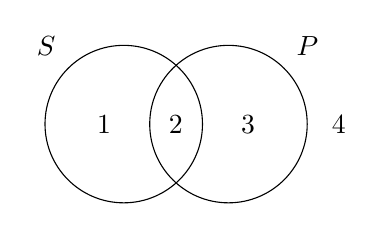
\begin{tikzpicture}
\def\firstcircle{(0,0) circle (1cm)}
\def\secondcircle{(0:1.33cm) circle (1cm)}
\draw \firstcircle node[outer sep=.75cm, above left] (s) {$S$} 
	node [xshift=-.25cm] (1) {1}
	node [xshift=.66cm] (2){2};
\draw \secondcircle node[outer sep=.75cm, above right] (p) {$P$}
	node [xshift=.25cm] (3) {3}
	node [xshift=1.4cm] (4){4};
\end{tikzpicture}
\end{center}

Now that we are considering arguments with three terms, we will need to draw three circles, and they need to overlap in a way that will let us represent the eight possible ways an individual can be inside or outside these three classes.

\begin{center}
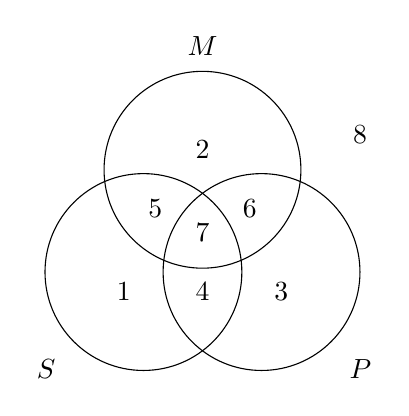
\begin{tikzpicture}
\def\firstcircle{(0,0) circle (1.25cm)}
\def\secondcircle{(60:1.5cm) circle (1.25cm)}
\def\thirdcircle{(0:1.5cm) circle (1.25cm)}

\draw \firstcircle node[outer sep=1cm, below left] {$S$}
	node [xshift=-.25cm, yshift=-.25cm](1) {1}
	node [xshift=.75cm, yshift=-.25cm] (4){4}
	node [xshift=.15cm, yshift=.8cm](5){5}
	node [xshift=.75cm, yshift=.5cm] (7){7};
\draw \secondcircle node [outer sep=1.33cm, above] {$M$}
	node [yshift=.25cm](2) {2};
\draw \thirdcircle node [outer sep=1cm, below right] {$P$}
	node [xshift=.25cm, yshift=-.25cm](3) {3}
	node[xshift=-.15cm, yshift=.8cm](6){6}
	node[xshift=1.25cm, yshift=1.75cm](8){8};  
\end{tikzpicture}
\label{fig:three_term_venn_areas}
\end{center}

So in this diagram, area 1 represents the things that are $S$ but not $M$ or $P$, area 2 represents the things that are $M$ but not $S$ or $P$, etc. 

As before, we represent universal statements by filling in the area that the statement says cannot be occupied. The only difference is that now there are more possibilities. So, for instance, there are now four mood-A propositions that can occur in the two premises. The major premise can either be ``All $P$ are $M$'' or ``All $M$ are $P$,'' and the minor premise can be either ``All $S$ are $M$'' or ``All $M$ are $S$.'' The Venn diagrams for those four sentences are given in the top two rows of Figure \ref{fig:mood-U_venns}.

Similarly, there are four mood-E propositions that can occur in the premises of an Aristotelian syllogism: ``No $P$ are $M$,'' ``No $M$ are $P$,'' ``No $S$ are $M$,'' and ``No $M$ are $S$.'' And again, we diagram these by shading out overlap between the two relevant circles. In this case, however, the first two statements are equivalent by conversion (see page \ref{defConversion}), as are the second two. Thus we only have two diagrams to worry about. See the bottom of Figure \ref{fig:mood-U_venns}


\begin{figure}
\begin{mdframed}[style=mytablebox]
\begin{tabu}{X[1,c,m]X[1,c,m]}

\multicolumn{2}{c}{\Large{Mood-A Statements}} \\


\multicolumn{2}{c}{\large{\emph{Major Premise}}} \\

\begin{center}
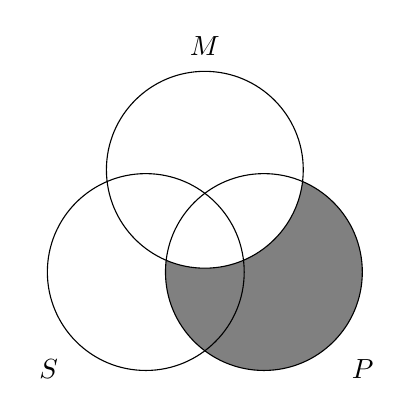
\begin{tikzpicture}
\def\firstcircle{(0,0) circle (1.25cm)}
\def\secondcircle{(60:1.5cm) circle (1.25cm)}
\def\thirdcircle{(0:1.5cm) circle (1.25cm)}

\begin{scope}[even odd rule] % Shade P without M
\clip \secondcircle (-1.5,-1.5) rectangle (2.75,2);
\fill[gray] \thirdcircle;
\end{scope}

\draw \firstcircle node[outer sep=1cm, below left] {$S$};
\draw \secondcircle node [outer sep=1.33cm, above] {$M$};
\draw \thirdcircle node [outer sep=1cm, below right] {$P$};
\end{tikzpicture}
\end{center}

&

\begin{center}
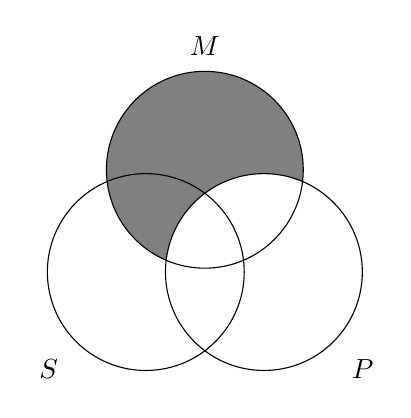
\begin{tikzpicture}
\def\firstcircle{(0,0) circle (1.25cm)}
\def\secondcircle{(60:1.5cm) circle (1.25cm)}
\def\thirdcircle{(0:1.5cm) circle (1.25cm)}

\begin{scope}[even odd rule] % Shade M without P
\clip \thirdcircle (-1.5,-1.5) rectangle (2,2.75);
\fill[gray] \secondcircle;
\end{scope}

\draw \firstcircle node[outer sep=1cm, below left] {$S$};
\draw \secondcircle node [outer sep=1.33cm, above] {$M$};
\draw \thirdcircle node [outer sep=1cm, below right] {$P$};

\end{tikzpicture}
\end{center}

\\

``All $P$ are $M$.'' 

&

``All $M$ are $P$.'' 

\\
\multicolumn{2}{c}{\large{\emph{Minor Premise}}} \\

\begin{center}
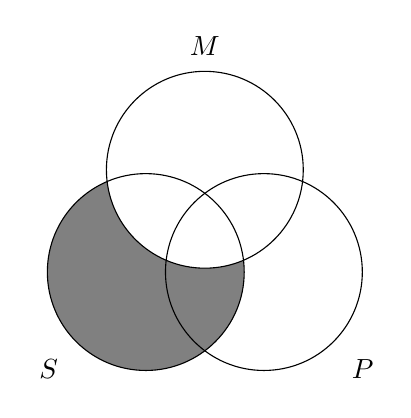
\begin{tikzpicture}
\def\firstcircle{(0,0) circle (1.25cm)}
\def\secondcircle{(60:1.5cm) circle (1.25cm)}
\def\thirdcircle{(0:1.5cm) circle (1.25cm)}

\begin{scope}[even odd rule] % Shade M without S
\clip \secondcircle (-1.5,-1.5) rectangle (2.75,2);
\fill[gray] \firstcircle;
\end{scope}

\draw \firstcircle node[outer sep=1cm, below left] {$S$};
\draw \secondcircle node [outer sep=1.33cm, above] {$M$};
\draw \thirdcircle node [outer sep=1cm, below right] {$P$};

\end{tikzpicture}
\end{center}

&

\begin{center}
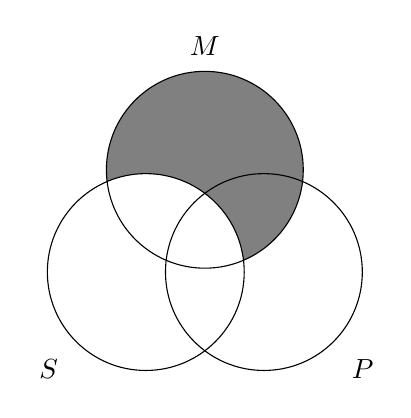
\begin{tikzpicture}
\def\firstcircle{(0,0) circle (1.25cm)}
\def\secondcircle{(60:1.5cm) circle (1.25cm)}
\def\thirdcircle{(0:1.5cm) circle (1.25cm)}

\begin{scope}[even odd rule] % Shade S without M
\clip \firstcircle (-1.5,-1.5) rectangle (2,2.75);
\fill[gray] \secondcircle;
\end{scope}

\draw \firstcircle node[outer sep=1cm, below left] {$S$};
\draw \secondcircle node [outer sep=1.33cm, above] {$M$};
\draw \thirdcircle node [outer sep=1cm, below right] {$P$};
\end{tikzpicture}
\end{center}

\\


``All $S$ are $M$.'' 
&
``All $M$ are $S$.'' 


\\
\\
\arrayrulecolor{gray}
\hline
\\

\multicolumn{2}{c}{\Large{Mood-E Statements}} \\

\large{\emph{Major Premise}}  & \large{\emph{Minor Premise}} \\

\begin{center}
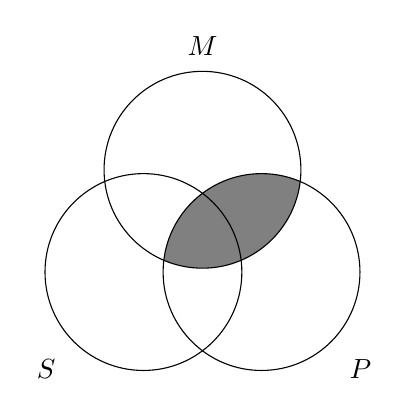
\begin{tikzpicture}
\def\firstcircle{(0,0) circle (1.25cm)}
\def\secondcircle{(60:1.5cm) circle (1.25cm)}
\def\thirdcircle{(0:1.5cm) circle (1.25cm)}

\begin{scope} %shade overlap between P and M
\clip \thirdcircle;
\fill[gray] \secondcircle;
\end{scope}


\draw \firstcircle node[outer sep=1cm, below left] {$S$};
\draw \secondcircle node [outer sep=1.33cm, above] {$M$};
\draw \thirdcircle node [outer sep=1cm, below right] {$P$};
\end{tikzpicture}
\end{center}

&

\begin{center}
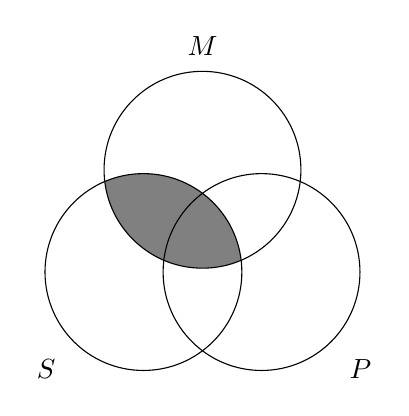
\begin{tikzpicture}
\def\firstcircle{(0,0) circle (1.25cm)}
\def\secondcircle{(60:1.5cm) circle (1.25cm)}
\def\thirdcircle{(0:1.5cm) circle (1.25cm)}

\begin{scope} %shade overlap between S and M
\clip \firstcircle;
\fill[gray] \secondcircle;
\end{scope}

\draw \firstcircle node[outer sep=1cm, below left] {$S$};
\draw \secondcircle node [outer sep=1.33cm, above] {$M$};
\draw \thirdcircle node [outer sep=1cm, below right] {$P$};
\end{tikzpicture}
\end{center}

\\


``No $M$ are $P$'' or 
``No $P$ are $M$.''

&

``No $M$ are $S$'' or ``No $S$ are $M$.''

\end{tabu}
\end{mdframed}
\caption{Venn diagrams for the eight universal statements that can occur in the premises.} \label{fig:mood-U_venns}
\end{figure}

Particular propositions are a bit trickier. Consider the statement ``Some $M$ are $P$.'' With a two circle diagram, you would just put an x in the overlap between the $M$ circle and the $P$ circle. But with the three circle diagram, there are now two places we can put it. It can go in either area 6 or area 7: 

\begin{center}
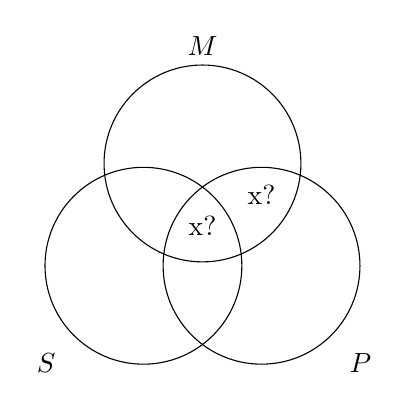
\begin{tikzpicture}
\def\firstcircle{(0,0) circle (1.25cm)}
\def\secondcircle{(60:1.5cm) circle (1.25cm)}
\def\thirdcircle{(0:1.5cm) circle (1.25cm)}

\draw \firstcircle node[outer sep=1cm, below left] {$S$}
	node [xshift=.75cm, yshift=.5cm] (7){x?};
\draw \secondcircle node [outer sep=1.25cm, above] {$M$};
\draw \thirdcircle node [outer sep=1cm, below right] {$P$}
	node[yshift=.9cm](6){x?};
\end{tikzpicture}
\end{center}

The solution here will be to put the x on the boundary between areas 6 and 7, to represent the fact that it could go in either location. 

\begin{center}
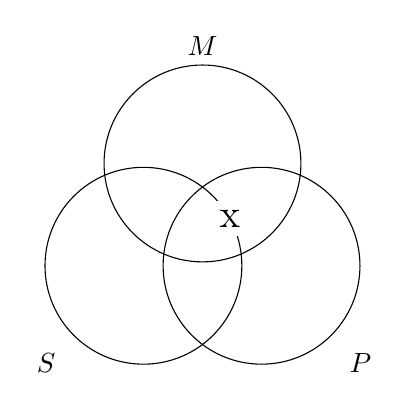
\begin{tikzpicture}
\def\firstcircle{(0,0) circle (1.25cm)}
\def\secondcircle{(60:1.5cm) circle (1.25cm)}
\def\thirdcircle{(0:1.5cm) circle (1.25cm)}
\draw \firstcircle node[outer sep=1cm, below left] {$S$}
	node [xshift=1.1cm, yshift=.6cm, fill=white] (7){\Large{x}};
\draw \secondcircle node [outer sep=1.25cm, above] {$M$};
\draw \thirdcircle node [outer sep=1cm, below right] {$P$};
\end{tikzpicture}
\end{center}

Sometimes, however, you won't have to draw the x on a border between two areas, because you will already know that one of those areas can't be occupied. Suppose, for instance, that you want to diagram ``Some $M$ are $P$,'' but you already know that all $M$ are $S$. You would diagram ``All $M$ are $S$'' like this:

\begin{center}
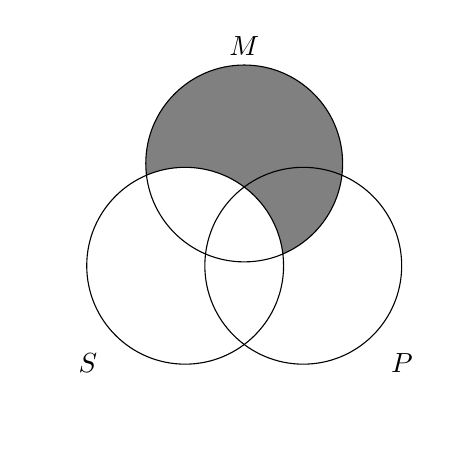
\begin{tikzpicture}
\def\firstcircle{(0,0) circle (1.25cm)}
\def\secondcircle{(60:1.5cm) circle (1.25cm)}
\def\thirdcircle{(0:1.5cm) circle (1.25cm)}

\begin{scope}[even odd rule] % Shade M without S
\clip \firstcircle (-2,-2) rectangle (2,2.6);
\fill[gray] \secondcircle;
\end{scope}

\draw \firstcircle node[outer sep=1cm, below left] {$S$};
\draw \secondcircle node [outer sep=1.25cm, above] {$M$};
\draw \thirdcircle node [outer sep=1cm, below right] {$P$};
\end{tikzpicture}
\end{center}

Then, when it comes time to add the x for ``Some $M$ are $P$,'' you know that it has to go in the exact center of the diagram:

\begin{center}
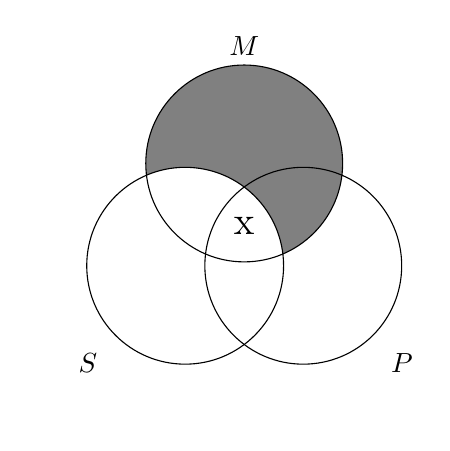
\begin{tikzpicture}
\def\firstcircle{(0,0) circle (1.25cm)}
\def\secondcircle{(60:1.5cm) circle (1.25cm)}
\def\thirdcircle{(0:1.5cm) circle (1.25cm)}

\begin{scope}[even odd rule] % Shade M without S
\clip \firstcircle (-2,-2) rectangle (2,2.6);
\fill[gray] \secondcircle;
\end{scope}

\draw \firstcircle node[outer sep=1cm, below left] {$S$}
	node [xshift=.75cm, yshift=.5cm, fill=white] (7){\Large{x}};
\draw \secondcircle node [outer sep=1.25cm, above] {$M$};
\draw \thirdcircle node [outer sep=1cm, below right] {$P$};
\end{tikzpicture}
\end{center}

The Venn diagrams for the particular premises that can appear in Aristotelian syllogisms are given in Figure \ref{fig:part_venns}. The figure assumes that you are just representing the individual premises, and don't know any other premises that would shade some regions out. Again, some of these premises are equivalent by conversion, and thus share a Venn diagram.

\begin{figure}
\begin{mdframed}[style=mytablebox]
\begin{tabu}{X[1,c,m]X[1,c,m]}

\multicolumn{2}{c}{\Large{Mood-I Statements}} \\

\large{\emph{Major Premise}}  & \large{\emph{Minor Premise}} \\

\begin{center}
\begin{tikzpicture}
\def\firstcircle{(0,0) circle (1.25cm)}
\def\secondcircle{(60:1.5cm) circle (1.25cm)}
\def\thirdcircle{(0:1.5cm) circle (1.25cm)}


\draw \firstcircle node[outer sep=1cm, below left] {$S$};
\draw \secondcircle node [outer sep=1.33cm, above] {$M$};
\draw \thirdcircle node [outer sep=1cm, below right] {$P$}
	node [xshift=-.5cm, yshift=.6cm, fill=light-gray] (7){\Large{x}};
\end{tikzpicture}
\end{center}

&

\begin{center}
\begin{tikzpicture}
\def\firstcircle{(0,0) circle (1.25cm)}
\def\secondcircle{(60:1.5cm) circle (1.25cm)}
\def\thirdcircle{(0:1.5cm) circle (1.25cm)}


\draw \firstcircle node[outer sep=1cm, below left] {$S$};
\draw \secondcircle node [outer sep=1.33cm, above] {$M$};
\draw \thirdcircle node [outer sep=1cm, below right] {$P$}
	node [xshift=-1.1cm, yshift=.6cm, fill=light-gray] (7){\Large{x}};
\end{tikzpicture}
\end{center}

\\


``Some $M$ are $P$'' or 
``Some $P$ are $M$.''

&

``Some $M$ are $S$'' or ``Some $S$ are $M$.''


\\
\\
\arrayrulecolor{gray}
\hline
\\


\multicolumn{2}{c}{\Large{Mood-O Statements}} \\


\multicolumn{2}{c}{\large{\emph{Major Premise}}} \\

\begin{center}
\begin{tikzpicture}
\def\firstcircle{(0,0) circle (1.25cm)}
\def\secondcircle{(60:1.5cm) circle (1.25cm)}
\def\thirdcircle{(0:1.5cm) circle (1.25cm)}

\draw \firstcircle node[outer sep=1cm, below left] {$S$};
\draw \secondcircle node [outer sep=1.33cm, above] {$M$};
\draw \thirdcircle node [outer sep=1cm, below right] {$P$}
	node [xshift=-.5cm, yshift=-.6cm, fill=light-gray] (7){\Large{x}};
\end{tikzpicture}
\end{center}

&

\begin{center}
\begin{tikzpicture}
\def\firstcircle{(0,0) circle (1.25cm)}
\def\secondcircle{(60:1.5cm) circle (1.25cm)}
\def\thirdcircle{(0:1.5cm) circle (1.25cm)}

\draw \firstcircle node[outer sep=1cm, below left] {$S$};
\draw \secondcircle node [outer sep=1.33cm, above] {$M$};
\draw \thirdcircle node [outer sep=1cm, below right] {$P$}
	node [xshift=-1.1cm, yshift=1.1cm, fill=light-gray] (7){\Large{x}};

\end{tikzpicture}
\end{center}

\\

``Some $P$ are not $M$.'' 

&

``Some $M$ are not $P$.'' 

\\
\multicolumn{2}{c}{\large{\emph{Minor Premise}}} \\

\begin{center}
\begin{tikzpicture}
\def\firstcircle{(0,0) circle (1.25cm)}
\def\secondcircle{(60:1.5cm) circle (1.25cm)}
\def\thirdcircle{(0:1.5cm) circle (1.25cm)}

\draw \firstcircle node[outer sep=1cm, below left] {$S$};
\draw \secondcircle node [outer sep=1.33cm, above] {$M$};
\draw \thirdcircle node [outer sep=1cm, below right] {$P$}
	node [xshift=-1cm, yshift=-.6cm, fill=light-gray] (7){\Large{x}};

\end{tikzpicture}
\end{center}

&

\begin{center}
\begin{tikzpicture}
\def\firstcircle{(0,0) circle (1.25cm)}
\def\secondcircle{(60:1.5cm) circle (1.25cm)}
\def\thirdcircle{(0:1.5cm) circle (1.25cm)}

\draw \firstcircle node[outer sep=1cm, below left] {$S$};
\draw \secondcircle node [outer sep=1.33cm, above] {$M$};
\draw \thirdcircle node [outer sep=1cm, below right] {$P$}
	node [xshift=-.1cm, yshift=1.2cm, fill=light-gray] (7){\Large{x}};


\end{tikzpicture}
\end{center}

\\


``Some $S$ are not $M$.'' 
&
``Some $M$ are not $S$.'' 



\end{tabu}
\end{mdframed}
\caption{Venn diagrams for the eight particular statements that can occur in the premises.} \label{fig:part_venns}
\end{figure}


\subsection{Venn Diagrams for Full Syllogisms}

In the last chapter, we used Venn diagrams to evaluate arguments with single premises. It turned out that when those arguments were valid, the conclusion was logically equivalent to the premise, so they had the exact same Venn diagram. This time we have two premises to diagram, and the conclusion won't be logically equivalent to either of them. Nevertheless we will find that for valid arguments, once we have diagrammed the two premises, we will also have diagrammed the conclusion.

First we need to specify a rule about the order to diagram the premises in: if one of the premises is universal and the other is particular, diagram the universal one first. This will allow us to narrow down the area where we need to put the x from the particular premise, as in the example above where we diagrammed ``Some $M$ are $P$'' assuming that we already knew that all $M$ are $S$. 

Let's start with a simple example, an argument with the form AAA-1. 

\begin{earg}
\item[P$_1$:] All $M$ are $P$.
\item[P$_2$:] All $S$ are $M.$
\vspace{-.5em}
\item [] \rule{0.3\linewidth}{.5pt} 
\item[C:] All $S$ are $P$.
\end{earg} 

Since both premises are universal, it doesn't matter what order we do them in. Let's do the major premise first. The major premise has us shade out the parts of the $M$ circle that don't overlap the $P$ circle, like this:

\begin{center}
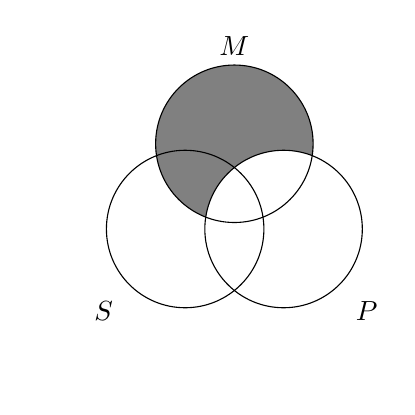
\begin{tikzpicture}
\def\firstcircle{(0,0) circle (1cm)}
\def\secondcircle{(60:1.25cm) circle (1cm)}
\def\thirdcircle{(0:1.25cm) circle (1cm)}
        \begin{scope}[even odd rule]
            \clip \thirdcircle (-2,-2) rectangle (2,2.5);
        \fill[gray] \secondcircle;
        \end{scope}
\draw \firstcircle node[outer sep=.8cm, below left] {$S$};
\draw \secondcircle node [outer sep=1cm, above] {$M$};
\draw \thirdcircle node [outer sep=.8cm, below right] {$P$};
\end{tikzpicture}
\end{center}

The second premise, on the other hand, tells us that there is nothing in the $S$ circle that isn't also in the $M$ circle. We put that together with the first diagram, and we get this:

\begin{center}
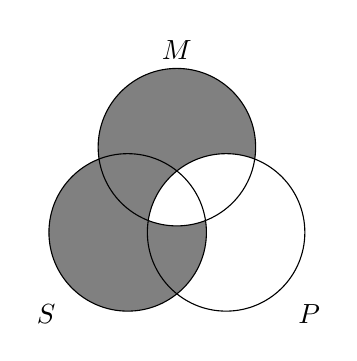
\begin{tikzpicture}
\def\firstcircle{(0,0) circle (1cm)}
\def\secondcircle{(60:1.25cm) circle (1cm)}
\def\thirdcircle{(0:1.25cm) circle (1cm)}

        \begin{scope}[even odd rule]
            \clip \thirdcircle (-1,-1) rectangle (2,2.6);
        \fill[gray] \secondcircle;
        \end{scope}

	\begin{scope}[even odd rule]
            \clip \secondcircle (-1,-1) rectangle (2,2);
        \fill[gray] \firstcircle;
        \end{scope}

\draw \firstcircle node[outer sep=.8cm, below left] {$S$};
\draw \secondcircle node [outer sep=1cm, above] {$M$};
\draw \thirdcircle node [outer sep=.8cm, below right] {$P$};
\end{tikzpicture}
\end{center}

From this we can see that the conclusion must be true. All $S$ are $P$, because the only space left in $S$ is the area in the exact center, area 7.

Now let's look at an argument that is invalid. One of the interesting things about the syllogism AAA-1 is that if you change the figure, it ceases to be valid. Consider AAA-2.

\begin{earg}
\item[P$_1$:] All $P$ are $M$.
\item[P$_2$:] All $S$ are $M$.
\vspace{-.5em}
\item [] \rule{0.2\linewidth}{.5pt} 
\item[C:] All $S$ are $P$.
\end{earg}

Again, both premises are universal, so we can do them in any order, so we will do the major premise first. This time, the major premise tells us to shade out the part of $P$ that does not overlap $M$.

\begin{center}
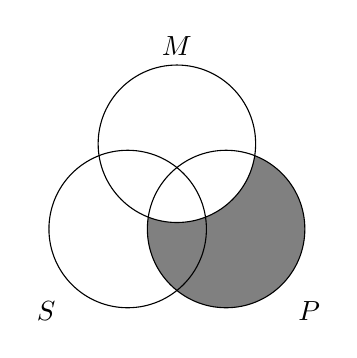
\begin{tikzpicture}
\def\firstcircle{(0,0) circle (1cm)}
\def\secondcircle{(60:1.25cm) circle (1cm)}
\def\thirdcircle{(0:1.25cm) circle (1cm)}
        \begin{scope}[even odd rule]
            \clip \secondcircle (-1,-1) rectangle (2.5,2);
        \fill[gray] \thirdcircle;
        \end{scope}
\draw \firstcircle node[outer sep=.8cm, below left] {$S$};
\draw \secondcircle node [outer sep=1cm, above] {$M$};
\draw \thirdcircle node [outer sep=.8cm, below right] {$P$};
\end{tikzpicture}
\end{center}

The second premise adds the idea that all $S$ are $M$, which we diagram like this:

\begin{center}
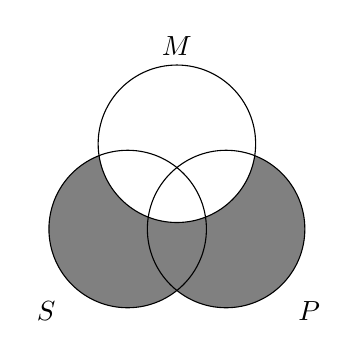
\begin{tikzpicture}
\def\firstcircle{(0,0) circle (1cm)}
\def\secondcircle{(60:1.25cm) circle (1cm)}
\def\thirdcircle{(0:1.25cm) circle (1cm)}
        \begin{scope}[even odd rule]
            \clip \secondcircle (-1,-1) rectangle (2.5,2);
        \fill[gray] \thirdcircle;
        \end{scope}
        
        \begin{scope}[even odd rule]
            \clip \secondcircle (-1,-1) rectangle (1,1);
        \fill[gray] \firstcircle;
        \end{scope}
        
\draw \firstcircle node[outer sep=.8cm, below left] {$S$};
\draw \secondcircle node [outer sep=1cm, above] {$M$};
\draw \thirdcircle node [outer sep=.8cm, below right] {$P$};
\end{tikzpicture}
\end{center}

Now we ask if the diagram of the two premises also shows that the conclusion is true. Here the conclusion is that all $S$ are $P$. If this diagram had made this true, we would have shaded out all the parts of $S$ that do not overlap $P$. But we haven't done that. It is still possible for something to be in area 5. Therefore this argument is invalid. 

Now let's try an argument with a particular statement in the premises. Consider the argument IAI-1:

\begin{earg}
\item[P$_1$:] Some $M$ are $P$.
\item[P$_2$:] All $S$ are $M$.
\vspace{-.5em}
\item [] \rule{0.2\linewidth}{.5pt} 
\item[C:] Some $S$ are $P$.
\end{earg} 

Here, the second premise is universal, while the first is particular, so we begin by diagramming the universal premise.

\begin{center}
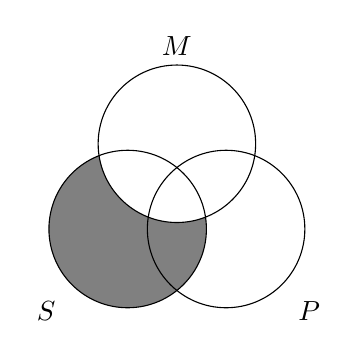
\begin{tikzpicture}
\def\firstcircle{(0,0) circle (1cm)}
\def\secondcircle{(60:1.25cm) circle (1cm)}
\def\thirdcircle{(0:1.25cm) circle (1cm)}

        \begin{scope}[even odd rule]
            \clip \secondcircle (-1,-1) rectangle (1,1);
        \fill[gray] \firstcircle;
        \end{scope}

\draw \firstcircle node[outer sep=.8cm, below left] {$S$};
\draw \secondcircle node [outer sep=1cm, above] {$M$};
\draw \thirdcircle node [outer sep=.8cm, below right] {$P$};
\end{tikzpicture}
\end{center}

Then we diagram the particular premise ``Some $M$ are $P$.'' This tells us that something is in the overlap between $M$ and $P$, but it doesn't tell us whether that thing is in the exact center of the diagram or in the area for things that are $M$ and $P$ but not $S$. Therefore, we place the x on the border between these two areas.

\begin{center}
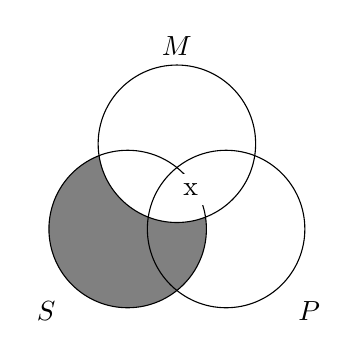
\begin{tikzpicture}
\def\firstcircle{(0,0) circle (1cm)}
\def\secondcircle{(60:1.25cm) circle (1cm)}
\def\thirdcircle{(0:1.25cm) circle (1cm)}

        \begin{scope}[even odd rule]
            \clip \secondcircle (-1,-1) rectangle (1,1);
        \fill[gray] \firstcircle;
        \end{scope}

\draw \firstcircle node[outer sep=.8cm, below left] {$S$};
\draw \secondcircle node [outer sep=1cm, above] {$M$};
\draw \thirdcircle node [outer sep=.8cm, below right] {$P$}
	node[xshift=-.45cm, yshift=.5cm, fill=white](6){x};
\end{tikzpicture}
\end{center}

Now we can see that the argument is not valid. The conclusion asserts that something is in the overlap between $S$ and $P$. But the x we drew does not necessarily represent an object that exists in that overlap. There is something out there that could be in area 7, but it could just as easily be in area 6. The second premise doesn't help us, because it just rules out the existence of objects in areas 1 and 4. 

For a final example, let's look at a case of a valid argument with a particular statement in the premises. If we simply change the figure of the argument in the last example from 1 to 3, we get a valid argument. This is the argument IAI-3:


\begin{earg}
\item[P$_1$:] Some $M$ are $P$.
\item[P$_2$:] All $M$ are $S$.
\vspace{-.5em}
\item [] \rule{0.3\linewidth}{.5pt} 
\item[C:] Some $S$ are $P$.
\end{earg} 

Again, we begin with the universal premise. This time it tells us to shade out part of the $M$ circle. 

\begin{center}
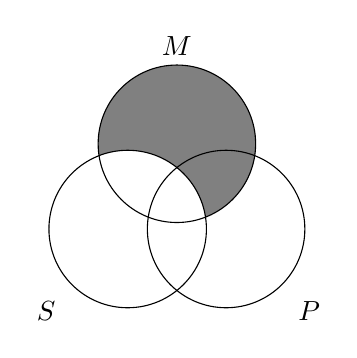
\begin{tikzpicture}
\def\firstcircle{(0,0) circle (1cm)}
\def\secondcircle{(60:1.25cm) circle (1cm)}
\def\thirdcircle{(0:1.25cm) circle (1cm)}

        \begin{scope}[even odd rule]
            \clip \firstcircle (-1,-1) rectangle (2,2.1);
        \fill[gray] \secondcircle;
        \end{scope}

\draw \firstcircle node[outer sep=.8cm, below left] {$S$};
\draw \secondcircle node [outer sep=1cm, above] {$M$};
\draw \thirdcircle node [outer sep=.8cm, below right] {$P$};
\end{tikzpicture}
\end{center}

But now we fill in the parts of $M$ that don't overlap with $S$, we have to put the x in the exact center of the diagram.


\begin{center}
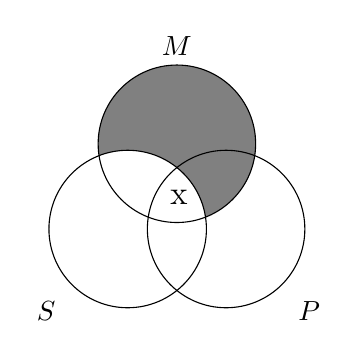
\begin{tikzpicture}
\def\firstcircle{(0,0) circle (1cm)}
\def\secondcircle{(60:1.25cm) circle (1cm)}
\def\thirdcircle{(0:1.25cm) circle (1cm)}

        \begin{scope}[even odd rule]
            \clip \firstcircle (-1,-1) rectangle (2,2.1);
        \fill[gray] \secondcircle;
        \end{scope}

\draw \firstcircle node[outer sep=.8cm, below left] {$S$};
\draw \secondcircle node [outer sep=1cm, above] {$M$};
\draw \thirdcircle node [outer sep=.8cm, below right] {$P$}
	node [xshift=-.6cm, yshift=.4cm] (7){\large{x}};
\end{tikzpicture}
\end{center}


And now this time we see that ``Some $S$ are $P$'' has to be true based on the premises, because the X has to be in area 7. So this argument is valid.                                 
                                               
\newglossaryentry{conditional validity}
{
name=conditional validity,
description={A kind if validity that Aristotelian syllogisms have if they are valid only given the assumption that the objects named by its terms actually exist.}
}

\newglossaryentry{unconditional validity}
{
name=unconditional validity,
description={A kind of validity that an Aristotelian syllogism has regardless of whether the objects named by its terms actually exist.}
}
                                                                                                    
Using this method, we can show that 15 of the 256 possible syllogisms are valid. Remember, however, that the Venn diagram method uses Boolean assumptions about existential import. If you make other assumptions about existential import, you will allow more valid syllogisms, as we will see in the next section. The additional syllogisms we will be able to prove valid in the next section will be said to have \textsc{\gls{conditional validity}} \label{def:Conditional_validity} because they are valid on the condition that the objects talked about in the universal statements actually exist. The 15 syllogisms that we can prove valid using the Venn diagram method have \textsc{\gls{unconditional validity}}. \label{def:Unconditional_validity} These syllogisms are given in Table \ref{tab:unconditionally_valid}. 

\begin{table}
\begin{mdframed}[style=mytablebox]
\begin{tabu}{X[1,c,m]X[1,c,m]X[1,c,m]X[1,c,m]}
\rowfont\bfseries
Figure 1 		& Figure 2 			& Figure 3 		& Figure 4 \\
%\endhead 
Barbara (AAA) 	& Camestres (AEE) 	& Disamis (IAI) 	& Calemes (AEE) \\
Celarent (EAE) 	& Cesare (EAE) 	& Bocardo (OAO)	& Dimatis (IAI) \\
Ferio (EIO)		& Festino (EIO) 	& Ferison (EIO) 	& Fresison (EIO) \\
Darii (AII)		& Baroco (AOO) 	& Datisi (AII) 	 & \\
\end{tabu}
\end{mdframed}
\caption{The 15 unconditionally valid syllogisms.}
\label{tab:unconditionally_valid}
% the version of the naming scheme used here is just the one from wikipedia. Hurley gives a version of the poem, but doesn't say which one it is. He also doesn't use the names as he goes along. Hurley's list differs from the wikipedia list on three names: Ferioque for Ferio, Camenes for Calemes, Dimaris for Dimatis.
\end{table}

The names on Table \ref{tab:unconditionally_valid} come from the Christian part of the Aristotelian tradition, where thinkers were writing in Latin. Students in that part of the tradition learned the valid forms by giving each one a female name. The vowels in the name represented the mood of the syllogism. So B\textbf{a}rb\textbf{a}r\textbf{a} has the mood AAA, Fr\textbf{e}s\textbf{i}s\textbf{o}n has the mood EIO, etc. The consonants in each name were also significant: they related to a process the Aristotelians were interested in called reduction, where arguments in the later figures were shown to be equivalent to arguments in the first figure, which was taken to be more self-evident. We won't worry about reduction in this textbook, however. The names of the valid syllogisms were often worked into a mnemonic poem. The oldest known version of the poem appears in a late 13th century book called \textit{Introduction to Logic} by William of Sherwood (Sherwood c. \citeyear{sherwood1275}/1966). Figure \ref{fig:barbara,celarent} is an image of the oldest surviving manuscript of the poem, digitized by the Bibliothèque Nationale de France.

The columns in Table \ref{tab:unconditionally_valid} represent the four figures. Syllogisms with the same mood also appear in the same row. So the EIO sisters---Ferio, Festino, Ferison, and Fresison---fill up row 3.  Camestres and Calemes share row 1;  Celarent and Cesare share row 2; and Darii and Datisi share row 4.   

\begin{figure}
\begin{mdframed}[style=mytableclearbox]
\includegraphics*[scale=.75]{img/barbara,celarent,darii,ferio} 
\end{mdframed}
\caption{The oldest surviving version of the ``Barbara, Celarent...'' poem, from William of Sherwood (c. \citeyear{sherwood1275}/1966)}
\label{fig:barbara,celarent}
\end{figure}


%%%%%%%%%	 Practice problems %%%%%%%%%%%

\practiceproblems
\label{venn_proofs}
\problempart Use Venn diagrams to determine whether the following Aristotelian syllogisms are valid. You can check your answers against Table \ref{tab:unconditionally_valid}.

\begin{longtabu}{X[1,l,p]X[9,l,p]} 
\textbf{Example}: &All $P$ are $M$ and no $M$ are $S$. Therefore, no $S$ are $P$. \\ 
\textbf{Answer}: &Valid (Calemes, AEE-4) \\
&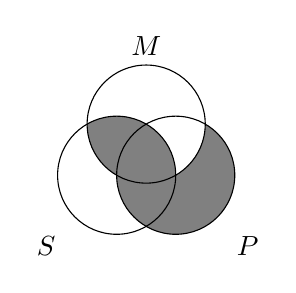
\begin{tikzpicture}
\def\firstcircle{(0,0) circle (.75cm)}
\def\secondcircle{(60:.75cm) circle (.75cm)}
\def\thirdcircle{(0:.75cm) circle (.75cm)}

	\begin{scope}[even odd rule] % Shade P without M
            \clip \secondcircle (-1,-1) rectangle (1.5,1.5);
        \fill[gray] \thirdcircle;
        \end{scope}

    \begin{scope} %shade overlap between S and M
      \clip \firstcircle;
      \fill[gray] \secondcircle;
    \end{scope}

\draw \firstcircle node[outer sep=.66cm, below left] {$S$};
\draw \secondcircle node [outer sep=.75cm, above] {$M$};
\draw \thirdcircle node [outer sep=.66cm, below right] {$P$};
\end{tikzpicture}\\ 
\end{longtabu} 

\begin{exercises}

\item Some $P$ are not $M$, and no $M$ are $S$. Therefore, some $S$ are $P$.
\answer{\\
\begin{venns}
\shadeintersectred{\middlecircle}{\subjectcircle}
\drawsubsyl
\drawmidsyl
\drawpredsyl
\someexistthreefour
\end{venns}
\\
OEI-IV Invalid 
}

\item All $M$ are $P$, and some $M$ are $S$. Therefore some $S$ are $P$. 
\answer{\\
\begin{venns}
\shadecomplementred{\middlecircle}{\middlesquare}{\predicatecircle}
\drawsubsyl
\drawmidsyl
\drawpredsyl
\someexistseven
\end{venns}
\\
Datisi (AII-3) Valid 
} 

\item No $P$ are $M$, and some $S$ are $M$. Therefore, some $S$ are not $P$.
\answer{\\
\begin{venns}
\shadeintersectred{\predicatecircle}{\middlecircle}
\drawsubsyl
\drawmidsyl
\drawpredsyl
\someexistfive
\end{venns}
\\
Festino (EIO-II) Valid 
} 
      
\item No $M$ are $P$, and all $S$ are $M$. Therefore, no $S$ are $P$.
\answer{\\
\begin{venns}
\shadeintersectred{\middlecircle}{\predicatecircle}
\shadecomplementred{\subjectcircle}{\subjectsquare}{\middlecircle}
\drawsubsyl
\drawmidsyl
\drawpredsyl
\end{venns}
\\
Celarent (EAE-I) Valid 
} 
\item All $M$ are $P$, and no $M$ are $S$. Therefore, all $S$ are $P$.
\answer{\\
\begin{venns}
\shadecomplementred{\middlecircle}{\middlesquare}{\predicatecircle}
\shadeintersectred{\middlecircle}{\subjectcircle}
\drawsubsyl
\drawmidsyl
\drawpredsyl
\end{venns}
\\
AEA-III Invalid 
} 
\item Some $M$ are not $P$, and some $M$ are $S$. Therefore, all $S$ are $P$.
\answer{\\
\begin{venns}
\drawsubsyl
\drawmidsyl
\drawpredsyl
\someexisttwofive
\someexistonefour
\end{venns}
\\

 OIA-III Invalid 
} 
 
\item No $P$ are $M$, and some $S$ are not $M$. Therefore, some $S$ are not $P$.
\answer{\\
\begin{venns}
\shadeintersectred{\predicatecircle}{\middlecircle}
\drawsubsyl
\drawmidsyl
\drawpredsyl
\someexistonefour
\end{venns}
\\
EOO-II Invalid 
}
 
\item Some $P$ are $M$, and some $S$ are $M$. Therefore, no $S$ are $P$.
\answer{\\
\begin{venns}
\drawsubsyl
\drawmidsyl
\drawpredsyl
\someexistsixseven
\someexistfiveseven
\end{venns}
\\
IIE-II Invalid 
}

\item No $P$ are $M$, and all $S$ are $M$. Therefore no $S$ are $P$.
\answer{\\
\begin{venns}
\shadeintersectred{\predicatecircle}{\middlecircle}
\shadecomplementred{\subjectcircle}{\subjectsquare}{\middlecircle}
\drawsubsyl
\drawmidsyl
\drawpredsyl
\end{venns}
\\
Cesare (EAE-II) Valid 
}  
\item No $M$ are $P$ and all $S$ are $M$. Therefore some $S$ are not $P$
\answer{\\
\begin{venns}
\shadeintersectred{\predicatecircle}{\middlecircle}
\shadecomplementred{\subjectcircle}{\subjectsquare}{\middlecircle}

\drawsubsyl
\drawmidsyl
\drawpredsyl
\end{venns}
\\
EAO-1 Invalid \\
As we will learn in the next section, this argument would be valid if we added the premise ``Some $S$ exist.'' As a result, we will say this form is ``conditionally valid''
}
\end{exercises}

\noindent \problempart Use Venn diagrams to determine whether the following Aristotelian syllogisms are valid. You can check your answers against Table \ref{tab:unconditionally_valid}.

\begin{exercises}

\item No $M$ are $P$, and some $M$ are $S$. Therefore some $S$ are not $P$.
\answer{\\Ferison (EIO-III)} 

\item Some $M$ are not $P$, and all $M$ are $S$. Therefore some $S$ are not $P$.
\answer{\\Bocardo (OAO-3)}
 
\item   No $M$ are $P$, and some $S$ are $M$. Therefore, some $S$ are not $P$.
 \answer{\\Ferio (EIO-I)}
 
\item All $M$ are $P$, and some $S$ are not $M$. Therefore, some $S$ are $P$.
\answer{\\AOI-I Invalid} 
 
\item Some $P$ are $M$, and all $M$ are $S$. Therefore some $S$ are $P$.
 \answer{\\Dimatis (IAI-IV)} 
 
\item Some $M$ are $P$, and all $S$ are $M$. Therefore, all $S$ are $P$.
\answer{\\IAA-I Invalid }
 
\item All $P$ are $M$, and all $M$ are $S$. Therefore, some $S$ are $P$.
\answer{\\AAI-IV Invalid }

 \item  All $P$ are $M$, and some $S$ are not $M$. Therefore, some $S$ are not $P$. 
 \answer{\\Baroco (AOO-II)}

\item No $P$ are $M$, and all $M$ are $S$. Therefore no $S$ are $P$.
\answer{\\EAE-IV Invalid} 
 
\item Some $P$ are $M$, and some $S$ are $M$. Therefore, some $S$ are $P$.
\answer{\\III-II Invalid} 
 \end{exercises}

\noindent\problempart The arguments below are missing conclusions. Use Venn diagrams to determine what conclusion can be drawn from the two premises. If no conclusion can be drawn, write ``No conclusion.'' \label{no_conclusion_set1}

\begin{longtabu}{p{.15\linewidth}p{.85\linewidth}} 
\textbf{Example 1}: & No $P$ are $M$ and some $M$ are not $S$. Therefore \underline{\hspace{2cm}} \\
\textbf{Answer}: & No conclusion\\
& 

\begin{venns}
\shadeintersect{\predicatecircle}{\middlecircle}
\someexisttwo
\drawsubsyl
\drawmidsyl
\drawpredsyl
\end{venns} 
\\
\textbf{Example 2}: & No $P$ are $M$ and  All $S$ are $M$. Therefore \underline{\hspace{2cm}} \\
\textbf{Answer}: &  No $S$ are $P$\\
& 

\begin{venns}
\shadeintersect{\predicatecircle}{\middlecircle}
\shadecomplement{\subjectcircle}{\subjectsquare}{\middlecircle}
\drawsubsyl
\drawmidsyl
\drawpredsyl
\end{venns}

\end{longtabu} 

\begin{exercises} 
 
\item All $M$ are $P$, and all $S$ are $M$. Therefore \underline{\hspace{2cm}}.
\answer{ \hspace{-2.4cm} All $S$ are $P$. \\
\begin{venns}
\shadecomplementred{\middlecircle}{\middlesquare}{\predicatecircle}
\shadecomplementred{\subjectcircle}{\subjectsquare}{\middlecircle}
\drawsubsyl
\drawmidsyl
\drawpredsyl
\end{venns}
\\ Barbara (AAA-I) 
} 

\item All $M$ are $P$, and some $M$ are $S$. Therefore \underline{\hspace{2cm}}. 
\answer{\hspace{-2.4cm} Some $S$ are $P$. \\
\begin{venns}
\shadecomplementred{\middlecircle}{\middlesquare}{\predicatecircle}
\drawsubsyl
\drawmidsyl
\drawpredsyl
\someexistseven
\end{venns}
\\Datisi (AII-3) 
} 

\item No $M$ are $P$ and some $S$ are not $M$. Therefore \underline{\hspace{2cm}}. 
\answer{ \hspace{-2.4cm} No conclusion \\
\begin{venns}
\shadeintersectred{\middlecircle}{\predicatecircle}
\drawsubsyl
\drawmidsyl
\drawpredsyl
\someexistonefour
\end{venns}
 \\ EO?-I Invalid 
 }
\item Some $M$ are $P$, and some $S$ are $M$. Therefore \underline{\hspace{2cm}}. 
\answer{ \hspace{-2.4cm} No conclusion \\
\begin{venns}
\drawsubsyl
\drawmidsyl
\drawpredsyl
\someexistsixseven
\someexistfiveseven
\end{venns}
\\  IE?-I Invalid 
} 
\item Some $P$ are $M$, and all $M$ are $S$. Therefore \underline{\hspace{2cm}}. 
\answer{\hspace{-2.4cm} No conclusion. \\
\begin{venns}
\shadecomplementred{\middlecircle}{\middlesquare}{\subjectcircle}
\drawsubsyl
\drawmidsyl
\drawpredsyl
\someexistfourseven
\end{venns}
\\ IA?-IV Invalid 
 }
\item All $P$ are $M$ and no $M$ are $S$. Therefore \underline{\hspace{2cm}} .
\answer{\hspace{-2.4cm} No $S$ are $P$. \\
\begin{venns}
\shadecomplementred{\predicatecircle}{\predicatesquare}{\middlecircle}
\shadeintersectred{\subjectcircle}{\middlecircle}
\drawsubsyl
\drawmidsyl
\drawpredsyl
\end{venns}
\\Calemes (AEE-IV) 
}
 
\item No $M$ are $P$ and all $S$ are $M$. Therefore \underline{\hspace{2cm}} .
\answer{ \hspace{-2.4cm} No $S$ are $P$. \\
\begin{venns}
\shadeintersectred{\middlecircle}{\predicatecircle}
\shadecomplementred{\subjectcircle}{\subjectsquare}{\middlecircle}
\drawsubsyl
\drawmidsyl
\drawpredsyl
\end{venns}
\\ Celarent (EAE-I) 
} 

\item \label{itm:no_conclusion_set1_EEE} No $P$ are $M$, and no $M$ are $S$. Therefore \underline{\hspace{2cm}}.
\answer{\hspace{-2.4cm} No conclusion. \\
\begin{venns}
\shadeintersectred{\middlecircle}{\predicatecircle}
\shadeintersectred{\middlecircle}{\subjectcircle}
\drawsubsyl
\drawmidsyl
\drawpredsyl
\end{venns}
\\ EE?-4 Invalid  
 }
 
\item No $M$ are $P$, and some $S$ are $M$. Therefore \underline{\hspace{2cm}}.
\answer{\hspace{-2.4cm} Some $S$ are not $P$. \\
\begin{venns}
\shadeintersectred{\middlecircle}{\predicatecircle}
\drawsubsyl
\drawmidsyl
\drawpredsyl
\someexistfive
\end{venns}
\\ Valid Ferio (EIO-1) . 
}
\item Some $P$ are $M$, and some $S$ are $M$. Therefore \underline{\hspace{2cm}}. 
\answer{\hspace{-2.4cm} No conclusion. \\
\begin{venns}
\drawsubsyl
\drawmidsyl
\drawpredsyl
\someexistsixseven
\someexistfiveseven
\end{venns}
 \\II?-2 Invalid 
  }
  \end{exercises}

\noindent \problempart The arguments below are missing conclusions. Use Venn diagrams to determine what conclusion can be drawn from the two premises. If no conclusion can be drawn, write ``No conclusion.'' 

\begin{exercises} 
\item Some $P$ are not $M$, and all $M$ are $S$. Therefore, \underline{\hspace{2cm}}. 
 \answer{\\OAA-IV Invalid }
 
\item All $M$ are $P$, and some $S$ are $M$. Therefore \underline{\hspace{2cm}}. 
\answer{\\Darii (AII-1) (unconditionally valid) }
 
\item All $P$ are $M$, and some $S$ are not $M$. Therefore \underline{\hspace{2cm}}.
\answer{\\Baroco (AOO-II) (unconditionally valid)}
 
\item Some $P$ are $M$, and all $M$ are $S$. Therefore \underline{\hspace{2cm}}.
\answer{\\Dimatis (IAI-IV) (unconditionally valid) }
 
\item All $P$ are $M$, and some $M$ are not $S$. Therefore \underline{\hspace{2cm}}. 
\answer{\\AOA-IV Invalid}
 
\item No $M$ are $P$, and some $S$ are $M$. Therefore \underline{\hspace{2cm}}.
\answer{\\Ferio (EIO-I) (unconditionally valid)} 
 
\item No $P$ are $M$, and no $S$ are $M$. Therefore \underline{\hspace{2cm}}. 
 
\item Some $M$ are not $P$, and no $M$ are $S$. Therefore \underline{\hspace{2cm}}. 
 
\item No $P$ are $M$, and all $S$ are $M$. Therefore \underline{\hspace{2cm}}. 
\answer{\\EAA-II Invalid} 
  
\item No $M$ are $P$, and some $M$ are $S$. Therefore \underline{\hspace{2cm}}.
\answer{\\Ferison (EIO-III) (unconditionally valid)} 
 
\end{exercises}
    

\noindent\problempart
\label{ex_on_syllogism_patterns}
\answer{\\ The questions in this section were mostly meant to get you thinking about the issues we will be discussing in Section 5.4. Hopefully by looking for patterns in the 256 syllogisms, you can actually anticipate the rules we will demonstrate later on}

\begin{exercises}
\item Do you think there are any valid arguments in Aristotle's set of 256 syllogisms where both premises are particular? Why or why not? \label{itm:two_particulars} 
\answer{\\No. You can intuitively see why this is the case when you remember that two particular premises could just be telling you about the existence of one or two particular objects, and you aren't going to be able to infer any generalities or any information about other particular objects from those two. For a more formal proof of why this is so, see see the discussion of Derived Rule 1 on page \ref{derived_rule_1}.} 


\item Do you think there are any valid arguments in Aristotle's set of 256 syllogisms where both premises are negative? Why or why not?
\answer{\\No. You can see this by playing around with the Venn diagrams for negative statements, or by looking at the more formal proof of Rule 3 on page \ref{rule_3}.}

\item Can a valid argument have a negative statement in the conclusion, but only affirmative statements in the premises? Why or why not?
\answer{\\No. Again you can see this by playing around with Venn diagrams for negative statements, or by looking at the more formal proof of Rule 4 on page \ref{rule_4}}


\item Can a valid argument have an affirmative statement in the conclusion, but only one affirmative premise?  
\answer{\\No, for the reasons stated above.}

\item Can a valid argument have two universal premises and a particular conclusion? 
\answer{\\No, because the two universal statements do not have existential import, but the particular statement does. We will be talking more about this in the next section and in the proof of Rule 5 on page \ref{rule_5}.}
\end{exercises}

% **********************************************
% *   Existential Import and Conditionally Valid Forms   *
% **********************************************

\section{Existential Import and Conditionally Valid Forms}
\label{sec:conditionally_valid_forms}
In the last section, we mentioned that you can prove more syllogisms valid if you make different assumptions about existential import. Recall that a statement has existential import if, when you assert the statement, you are also asserting the existence of the things the statement talks about. (See page \pageref{def:Existential_import}.) So if you interpret a mood-A statement as having existential import, it not only asserts ``All $S$ is $P$,'' it also asserts ``$S$ exists.'' Thus the mood-A statement ``All unicorns have one horn'' is false, if it is taken to have existential import, because unicorns do not exist. It is probably  true, however, if you do not imagine the statement as having existential import. If anything is true of unicorns, it is that they would have one horn if they existed.

We saw in Section \ref{sec:ExistentialImport} that before Boole, Aristotelian thinkers had all sorts of opinions about existential import, or, as they put it, whether a term ``supposits.'' This generally led them to recognize additional syllogism forms as valid. You can see this pretty quickly if you just remember the traditional square of opposition. The traditional square allowed for many more valid immediate inferences than the modern square. It stands to reason that traditional ideas about existential import will also allow for more valid syllogisms. 

Our system of Venn diagrams can't represent all of the alternative ideas about existential import. For instance, it has no way of representing Ockham's belief that mood-O statements do \emph{not} have existential import. Nevertheless, it would be nice if we could expand our system of Venn diagrams to show that some syllogisms are valid if you make additional assumptions about existence. 

Consider the argument Barbari (AAI-1).

\begin{earg}
\item[P$_1$:] All $M$ are $P$.
\item[P$_2$:] All $S$ are $M$.
\vspace{-.5em}
\item [] \rule{0.2\linewidth}{.5pt} 
\item[C:] Some $S$ are $P$.
\end{earg} 
 
 
You won't find this argument in the list of unconditionally valid forms in Table \ref{tab:unconditionally_valid}. This is because under Boolean assumptions about existence it is not valid. The Venn diagram, which follows Boolean assumptions, shows this. 

\begin{center}
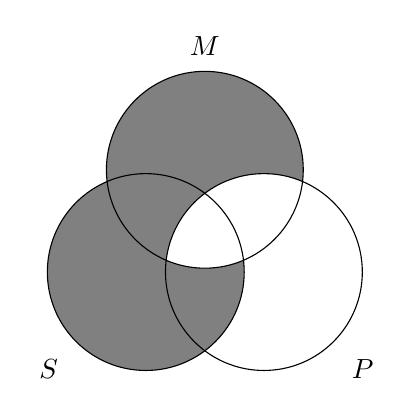
\begin{tikzpicture}
\def\firstcircle{(0,0) circle (1.25cm)}
\def\secondcircle{(60:1.5cm) circle (1.25cm)}
\def\thirdcircle{(0:1.5cm) circle (1.25cm)}

\begin{scope}[even odd rule] % Shade M without P
\clip \thirdcircle (-1,-1) rectangle (2,2.6);
\fill[gray] \secondcircle;
\end{scope}

\begin{scope}[even odd rule] % Shade S without M
\clip \secondcircle (-1.5,-1.5) rectangle (1.5,1.5);
\fill[gray] \firstcircle;
\end{scope}


\draw \firstcircle node[outer sep=1cm, below left] {$S$};
\draw \secondcircle node [outer sep=1.33cm, above] {$M$};
\draw \thirdcircle node [outer sep=1cm, below right] {$P$};
\end{tikzpicture}
\end{center}

This is essentially the same argument as Barbara, but the mood-A statement in the conclusion has been replaced by a mood-I statement. We can see from the diagram that the mood-A statement ``All $S$ are $P$'' is true. There is no place to put an $S$ other than in the overlap with $P$. But we don't actually know the mood-I statement ``Some $S$ is $P$,'' because we haven't drawn an x in that spot. Really, all we have shown is that \emph{if} an $S$ existed, it would be $P$. 

But by the traditional square of opposition (p. \pageref{fig:traditionalsquare}) we know that the mood-I statement is true. The traditional square, unlike the modern one, allows us to infer the truth of a particular statement given the truth of its corresponding universal statement. This is because the traditional square assumes that the universal statement has existential import. It is really two statements, ``All $S$ is $P$'' and ``Some $S$ exists.'' 

Because the mood-A statement is actually two statements on the traditional interpretation, we can represent it simply by adding an additional line to our argument. It is always legitimate to change an argument by making additional assumptions. The new argument won't have the exact same impact on the audience as the old argument. The audience will now have to accept an additional premise, but in this case all we are doing is making explicit an assumption that the Aristotelian audience was making anyway. The expanded argument will look like this:

 \begin{earg}
\item[P$_1$:] All $M$ are $P$.
\item[P$_2$:] All $S$ are $M$.
\item[P$_3$:] Some $S$ exists.*
\vspace{-.5em}
\item [] \rule{0.2\linewidth}{.5pt} 
\item[C:] Some $S$ are $P$
\end{earg} 
 
Here the asterisk indicates that we are looking at an implicit premise that has been made explicit.\iflabelexists{chap:incomplete_unclear_arguments}{This is similar to what we did in Chapter \ref{chap:incomplete_arguments} on adding warrants.}{} Now that we have an extra premise, we can add it to our Venn diagram. Since there is only one place for the $S$ to be, we know where to put our x. \label{CVFex1}

\begin{center}
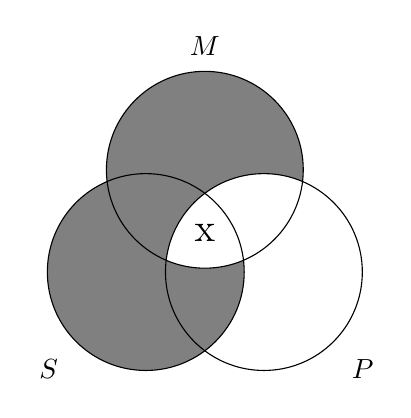
\begin{tikzpicture}
\def\firstcircle{(0,0) circle (1.25cm)}
\def\secondcircle{(60:1.5cm) circle (1.25cm)}
\def\thirdcircle{(0:1.5cm) circle (1.25cm)}

\begin{scope}[even odd rule] % Shade M without P
\clip \thirdcircle (-1,-1) rectangle (2,2.6);
\fill[gray] \secondcircle;
\end{scope}

\begin{scope}[even odd rule] % Shade S without M
\clip \secondcircle (-1.5,-1.5) rectangle (1.5,1.5);
\fill[gray] \firstcircle;
\end{scope}


\draw \firstcircle node[outer sep=1cm, below left] {$S$};
\draw \secondcircle node [outer sep=1.33cm, above] {$M$};
\draw \thirdcircle node [outer sep=1cm, below right] {$P$}
	node[xshift=-.75cm, yshift=.5cm](7){\Large{x}};
\end{tikzpicture}
\end{center}


\newglossaryentry{critical term}
{
name=critical term,
description={the term that names things that must exist in order for a conditionally valid argument to be actually valid.}
}

\

In this argument $S$ is what we call the ``critical term.'' The \gls{critical term} \label{def:critical_term} is the term that names things that must exist in order for a conditionally valid argument to be actually valid. In this argument, the critical term was $S$, but sometimes it will be $M$ or $P$. 

We have used Venn diagrams to show that Barbari is valid once you include the additional premise. Using this method we can identify nine more forms, on top of the previous 15, that are valid if we add the right existence assumptions (Table \ref{tab:full_twentyfour}) 

\begin{table}
\small
\begin{mdframed}[style=mytablebox]
\begin{longtabu}{X[1,c,m]X[10,c,m]X[11,c,m]X[10,c,m]X[10,c,m]X[6,c,m]}
\rowfont\bfseries 
&	Figure 1 		& Figure 2 			& Figure 3 		& Figure 4 & Condition \\
\endhead 
&&&&\\

\parbox[t]{2mm}{\multirow{4}{*}{\rotatebox{90}{\hspace{-2em}Unconditional}}} 

& Barbara (AAA) 	& Camestres (AEE)  	&  Disamis (IAI) 	& Calemes (AEE) \\

& Celarent (EAE) 	& Cesare (EAE) 	& Bocardo (OAO)	& Dimatis (IAI) \\

& Ferio (EIO)		& Festino (EIO) 	& Ferison (EIO) 	& Fresison (EIO) \\

& Darii (AII)		& Baroco (AOO) 	& Datisi (AII) 	 & \\

&&&&\\

\hline

&&&&\\

\parbox[t]{2mm}{\multirow{4}{*}{\rotatebox{90}{\hspace{-1em}Conditional}}}
& Barbari (AAI)		& Camestros (AEO)	&				&	Calemos (AEO)	& $S$ exists \\

& Celaront (EAO)	& Cesaro (EAO)	&				&			& $S$ exists \\

&					&					& Felapton (EAO)	& Fesapo (EAO)	& $M$ exists \\

&					&					& Darapti (AAI)		&  			& $M$ exists \\

&					&					& 					& Bamalip (AAI) 			& $P$ exists \\

\end{longtabu}
\end{mdframed}
\caption{All 24 Valid Syllogisms}
\label{tab:full_twentyfour}
\end{table}

Thus we now have an expanded method for evaluating arguments using Venn diagrams. To evaluate an argument, we first use a Venn diagram to determine whether it is unconditionally valid. If it is, then we are done. If it is not, then we see if adding an existence assumption can make it conditionally valid. If we can add such an assumption, add it to the list of premises and put an x in the relevant part of the Venn diagram. If we cannot make the argument valid by including additional existence assumptions, we say it is completely invalid.

Let's run through a couple examples. Consider the argument EAO-3.

\begin{earg}
\item[P$_1$:] No $M$ are $P$.
\item[P$_2$:] All $M$ are $S$.
\vspace{-.5em}
\item [] \rule{0.2\linewidth}{.5pt} 
\item[C:] Some $S$ are not $P$.   
\end{earg} 

First we use the regular Venn digram method to see whether the argument is unconditionally valid.

\begin{center}
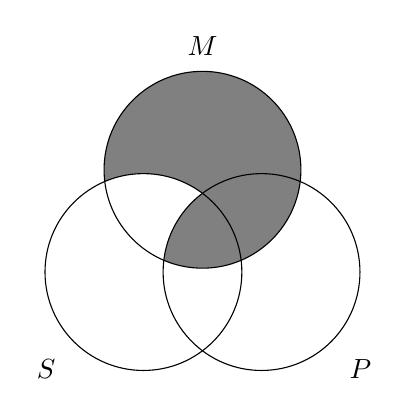
\begin{tikzpicture}
\def\firstcircle{(0,0) circle (1.25cm)}
\def\secondcircle{(60:1.5cm) circle (1.25cm)}
\def\thirdcircle{(0:1.5cm) circle (1.25cm)}

\begin{scope} %shade overlap between P and M
\clip \thirdcircle;
\fill[gray] \secondcircle;
\end{scope}

\begin{scope}[even odd rule] % Shade M without S
\clip \firstcircle (-1,-1) rectangle (2,2.75);
\fill[gray] \secondcircle;
\end{scope}


\draw \firstcircle node[outer sep=1cm, below left] {$S$};
\draw \secondcircle node [outer sep=1.33cm, above] {$M$};
\draw \thirdcircle node [outer sep=1cm, below right] {$P$};
\end{tikzpicture}
\end{center}

We can see from this that the argument is not valid. The conclusion says that some $S$ are not $P$, but we can't tell that from this diagram. There are three possible ways something could be $S$, and we don't know if any of them are occupied. 

Simply adding the premise $S$ exists won't help us, because we don't know whether to put the x in the overlap between $S$ and $M$, the overlap between $S$ and $P$, or in the area that is just $S$. Of course, we would want to put it in the overlap between $S$ and $M$, because that would mean that there is an $S$ that is not $P$. However, we can't justifying doing this simply based on the premise that $S$ exists. 

The premise that $P$ exists will definitely not help us. The $P$ would either go in the overlap between $S$ and $P$ or in the area that is only $P$. Neither of these would show ``Some $S$ is not $P$.''

The premise ``$M$ exists'' does the trick, however. If an $M$ exists, it has to also be $S$ but not $P$. And this is sufficient so show that some $S$ is not $P$. We can then add this additional premise to the argument to make it valid. \label{CVFex2}

\begin{earg}
\item[P$_1$:] No $M$ are $P$.
\item[P$_2$:] All $M$ are $S$.
\item[P$_3$:] $M$ exists.*
\vspace{-.5em}
\item [] \rule{0.2\linewidth}{.5pt} 
\item[C:] Some $S$ are not $P$.   
\end{earg} 

Checking it against Table \ref{tab:full_twentyfour}, we see that we were right: this is a conditionally valid argument named Felapton.

Now consider the argument EII-3:

\begin{earg} 
\item[P$_1$:] No $M$ are $P$.
\item[P$_2$:] Some $M$ are $S$.
\vspace{-.5em} 
\item [] \rule{0.2\linewidth}{.5pt} 
\item[C:] Some $S$ are $P$.
 \end{earg}

First we need to see if it is unconditionally valid. So we draw the Venn diagram. 

\begin{center}
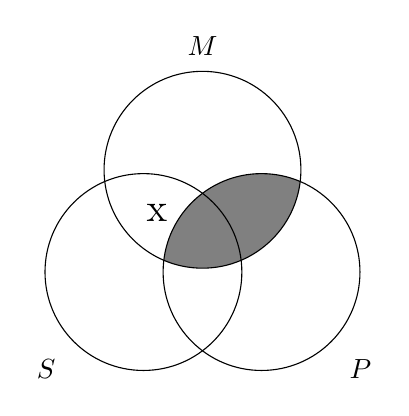
\begin{tikzpicture}

\def\firstcircle{(0,0) circle (1.25cm)}
\def\secondcircle{(60:1.5cm) circle (1.25cm)}
\def\thirdcircle{(0:1.5cm) circle (1.25cm)}

\begin{scope} %shade overlap between P and M
\clip \thirdcircle;
\fill[gray] \secondcircle;
\end{scope}

\draw \firstcircle node[outer sep=1cm, below left] {$S$};
\draw \secondcircle node [outer sep=1.33cm, above] {$M$};
\draw \thirdcircle node [outer sep=1cm, below right] {$P$}
	node[xshift=-1.33cm, yshift=.75cm](5){\Large{x}};
\end{tikzpicture}
\end{center}

The conclusion says that some $S$ are $P$, but we obviously don't know this from the diagram above. There is no x in the overlap between $S$ and $P$. Part of that region is shaded out, but the rest could go either way.

What about conditional validity? Can we add an existence assumption that would make this valid? Well, the x we have already drawn lets us know that both $S$ and $M$ exist, so it won't help to add those premises. What about adding $P$? That won't help either. We could add the premise ``$P$ exists'' but we wouldn't know whether that $P$ is in the overlap between $S$ and $P$ or in the area to the right, which is just $P$. \label{CVFex3}

Therefore this argument is invalid. And when we check the argument against Table \ref{tab:full_twentyfour}, we see that it is not present. 

\practiceproblems
\noindent \problempart Use Venn diagrams to determine whether the following arguments are unconditionally valid, conditionally valid, or invalid. If they are conditionally valid, write out the premise you need to add. You can check your answers against Table \ref{tab:full_twentyfour}.

\begin{longtabu}{p{.1\linewidth}p{.9\linewidth}} 
\textbf{Example}: & All $M$ are $P$ and all $M$ are $S$. Therefore some $S$ are $P$ \\
\textbf{Answer}: & Added premise: P$_3$: $M$ exists. \\
& \begin{center}
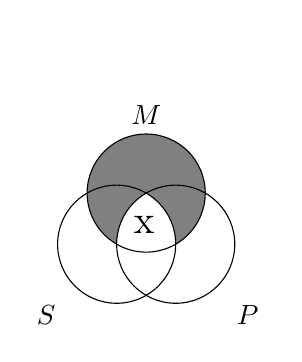
\begin{tikzpicture}
\def\firstcircle{(0,0) circle (.75cm)}
\def\secondcircle{(60:.75cm) circle (.75cm)}
\def\thirdcircle{(0:.75cm) circle (.75cm)}

\begin{scope}[even odd rule] % Shade M without P
\clip \thirdcircle (-1,-1) rectangle (2,2.75);
\fill[gray] \secondcircle;
\end{scope}


\begin{scope}[even odd rule] % Shade M without S
\clip \firstcircle (-1,-1) rectangle (2,2.75);
\fill[gray] \secondcircle;
\end{scope}


\draw \firstcircle node[outer sep=.66cm, below left] {$S$};
\draw \secondcircle node [outer sep=.75cm, above] {$M$};
\draw \thirdcircle node [outer sep=.66cm, below right] {$P$}
	node[xshift=-.4cm, yshift=.25cm](5){{\Large{x}}};
\end{tikzpicture}
\end{center}
\\ &
Conditionally valid (Darapti, AAI-3)
\end{longtabu} 

 
\begin{exercises} 
 
\item No $P$ are $M$, and all $S$ are $M$, so some $S$ are not $P$.
\answer{ \\
\begin{venns}

\shadeintersectred{\predicatecircle}{\middlecircle}
\shadecomplementred{\subjectcircle}{\subjectsquare}{\middlecircle}

\drawsubsyl
\drawmidsyl
\drawpredsyl

\end{venns}

Additional Premise: $S$ exists. 

Cesaro (EAO-1I, conditionally valid)  
\vspace{6pt}}
 
\item Some $P$ are $M$, and some $S$ are $M$. Therefore all $S$ are $P$.
\answer{ \\
\begin{venns}
\drawsubsyl
\drawmidsyl
\drawpredsyl
\someexistsixseven
\someexistfiveseven
\end{venns}

IIA-II Invalid 
\vspace{6pt}}

\item No $M$ are $P$, and some $S$ are $M$. Therefore, some $S$ are not $P$.
\answer{ \\
\begin{venns}
\shadeintersectred{\middlecircle}{\predicatecircle}
\someexistfive
\drawsubsyl
\drawmidsyl
\drawpredsyl

\end{venns}

Ferio (EIO-I, unconditionally valid) 
\vspace{6pt} }

\item  No $M$ are $P$, and all $S$ are $M$. Therefore, some $S$ are not $P$.
\answer{ \\
\begin{venns}
\shadeintersectred{\middlecircle}{\predicatecircle}
\shadecomplementred{\subjectcircle}{\subjectsquare}{\middlecircle}

\drawsubsyl
\drawmidsyl
\drawpredsyl

\end{venns}

Needed premise: Some $S$ exist.

Celaront (EAO-1, Conditionally valid) 
\vspace{6pt} }

\item No $P$ are $M$, and some $M$ are $S$, so some $S$ are not $P$.  
\answer{  \\
\begin{venns}

\shadeintersectred{\predicatecircle}{\middlecircle}

\drawsubsyl
\drawmidsyl
\drawpredsyl
\someexistfive

\end{venns}
\\Fresison (EIO-IV, unconditionally valid) 
\vspace{6pt} }
 
\item All $P$ are $M$, and all $M$ are $S$, so some $S$ are $P$.
\answer{ \\
\begin{venns}
\shadecomplementred{\predicatecircle}{\predicatesquare}{\middlecircle}
\shadecomplementred{\middlecircle}{\middlesquare}{\subjectcircle}
\drawsubsyl
\drawmidsyl
\drawpredsyl
\end{venns}
\\Needed premise: $P$ exists. \\
Bamalip (AAI-IV, conditionally valid) 
\vspace{6pt}  }

\item Some $P$ are not $M$, and some $M$ are $S$. Therefore all $S$ are $P$.
\answer{ \\
\begin{venns}

\drawsubsyl
\drawmidsyl
\drawpredsyl
\someexistthreefour
\someexistfiveseven
\end{venns}
\\ OIA-IV Invalid 7
 \vspace{6pt}}

\item No $P$ are $M$, and all $M$ are $S$. Therefore some $S$ are not $P$. 
\answer{ \\
 \begin{venns}
\shadeintersectred{\predicatecircle}{\middlecircle}
\shadecomplementred{\middlecircle}{\middlesquare}{\subjectcircle}
\drawsubsyl
\drawmidsyl
\drawpredsyl
\end{venns}
\\Needed premise: $P$ exists. \\ Fesapo (AEO-IV, conditionally valid) 
\vspace{6pt}} 

\item All $M$ are $P$, and no $S$ are $M$. Therefore, some $S$ are $P$.
\answer{ \\
 \begin{venns}
\shadecomplementred{\middlecircle}{\middlesquare}{\predicatecircle}
\shadeintersectred{\middlecircle}{\subjectcircle}
\drawsubsyl
\drawmidsyl
\drawpredsyl
\end{venns}
\\ AEI-I Invalid 
}
\item Some $M$ are $P$, and some $S$ are not $M$. Therefore, some $S$ are $P$.
\answer{ \\
\begin{venns}

\drawsubsyl
\drawmidsyl
\drawpredsyl
\someexistsixseven
\someexistonefour
\end{venns}
\\ IOI-I Invalid 
}
\end{exercises}
    
\noindent \problempart Use Venn diagrams to determine whether the following arguments are unconditionally valid, conditionally valid, or invalid. If they are conditionally valid, write out the premise you need to add. You can check your answers against Table \ref{tab:full_twentyfour}.

\begin{exercises} 

\item No $M$ are $P$, and all $M$ are $S$. Therefore some $S$ are not $P$.
\answer{Felapton (EAO-1II)  }
   
\item Some $M$ are $P$, and all $M$ are $S$. Therefore some $S$ are $P$.
\answer{Disamis (IAI-III) (unconditionally valid) }
 
\item All $M$ are $P$, and some $M$ are $S$, so no $S$ are $P$.
\answer{AIE-III Invalid }
 
    
\item No $M$ are $P$, and some $M$ are $S$, so some $S$ are not $P$. 
\answer{Ferison (EIO-III) (unconditionally valid) }
 
 
\item Some $P$ are $M$, and some $S$ are not $M$, so no $S$ are $P$
\answer{IOE-II Invalid} 
 
\item All $M$ are $P$, and all $S$ are $M$, so some $S$ are $P$. 
\answer{Barbari (AAI-I) (conditionally valid) }
 
\item All $P$ are $M$, and no $M$ are $S$, so no $S$ are $P$. 
\answer{Calemes (AEE-IV) (unconditionally valid) }
 
\item No $P$ are $M$, and all $S$ are $M$, so some $S$ are not $P$.
\answer{Camestros (EAO-1I) }
 
\item All $P$ are $M$, and no $M$ are $S$, so some $S$ are not $P$.  
\answer{Calemos (AEO-IV) }
 
\item All $M$ are $P$, and some $S$ are $M$, so some $S$ are $P$. 
\answer{Darii (AII-1) (unconditionally valid) }
 
\end{exercises}


% *******************************************
% *                  Rules and Fallacies                            *
% *******************************************

\section{Rules and Fallacies}
\label{sec:rules_and_fallacies}
Did you do the exercises in Part \ref{ex_on_syllogism_patterns} of Section \ref{sec:testing_validity}? If you didn't, go back and think about those questions now, before reading any further. The problem set had five general questions like, ``Can a valid argument have only negative premises?'' The point of those questions was to get you to think about what patterns might exist among the 256 Aristotelian syllogisms, and how those patterns might single out 24 syllogisms as the only ones that can be valid. 

In this section, we are going to answer the questions in Part \ref{ex_on_syllogism_patterns} in detail by identifying rules that all valid syllogisms amongst the 256 Aristotelian syllogisms must obey. Seeing these rules will help you understand the \emph{structure} of this part of logic. We aren't just  assigning the labels ``valid'' and ``invalid'' to arguments randomly. 

Each of the rules we will identify is associated with a fallacy. If you violate the rule, you commit the fallacy. These fallacies are like the fallacies that are identified in the parts of the complete version of this text on critical thinking, \nix{in Part \ref{part:CT_and_informal_logic}}\label{ver_var} in that they represent mistakes in reasoning. If you make an inference that commits one of these fallacies, you have used reasoning incorrectly. However, unlike the fallacies we looked at in the Critical Thinking section, many of these fallacies are not even tempting. They are not ways the human mind goes naturally off the rails. They are just things that you shouldn't do.   

In the next subsection we are going to outline five basic rules and the fallacies that go with them, along with an addition rule/fallacy pair that can be derived from the initial five. All standard logic textbooks these days use some version of these rules, although they might divide them up differently. Some textbooks also include rules that we have built into our definition of an Aristotelian syllogism in standard form. For instance, other textbooks might have a rule here saying valid syllogisms can't have four terms, or have to use terms in the same way each time. All of this is built into our definitions of an Aristotelian syllogism and standard form for such a syllogism, so we don't need to discuss them here. 

\subsection{Six Rules and Fallacies}
\begin{quotation}
\begin{longtabu}{p{.1\linewidth}p{.9\linewidth}}
\textbf{Rule 1}: & The middle term in a valid Aristotelian syllogism must be distributed at least once. 
\end{longtabu}
\end{quotation}

\newglossaryentry{fallacy of the undistributed middle}
{
name=fallacy of the undistributed middle,
description={A fallacy committed in an Aristotelian syllogism where the middle term is not distributed in either premise.}
}

Consider these two arguments:

\begin{tabu}{p{.5\linewidth}p{.5\linewidth}}

\begin{earg}
\item[P$_1$:] All $M$ are $P$.
\item[P$_2$:] All $S$ are $M$.
\vspace{-.5em}
\item [] \rule{0.4\linewidth}{.5pt} 
\item[C:] All $S$ are $P$.
\end{earg}

&

\begin{earg}
\item[P$_1$:] All $P$ are $M$.
\item[P$_2$:] All $S$ are $M$.
\vspace{-.5em}
\item [] \rule{0.4\linewidth}{.5pt} 
\item[C:] All $S$ are $P$.
\end{earg}

\end{tabu}

The syllogism on the left (Barbara) is obviously valid, but if you change it to figure 2, you get the syllogism on the right, which is obviously invalid. What causes this change?


The premises in the second syllogism say that $S$ and $P$ are both parts of $M$, but they no longer tell us anything about the relationship between $S$ and $P$. To see why this is the case, we need to bring back a term we saw on page \pageref{def:Distribution}, distribution. A term is distributed in a statement if the statement makes a claim about every member of that class. So in ``All $M$ are $P$'' the term $M$ is distributed, because the statement tells us something about every single $M$. They are all also $P$. The term $P$ is not distributed in this sentence, however. We do not know anything about every single $P$. We know that $M$ is in $P$, but not vice versa. 

In general mood-A statements distribute the subject, but not the predicate. This means that when we reverse $P$ and $M$ in the first premise, we create an argument where $S$ and $P$ are distributed, but $M$ is not. This means that the argument is always going to be invalid. 

This short argument can show us that arguments with an undistributed middle are always invalid: The conclusion of an Aristotelian syllogism tries to say something about the relationship between $S$ and $P$. It does this using the relationship those two terms have to the third term $M$. But if $M$ is never distributed, then $S$ and $P$ can be different, unrelated parts of $M$. Therefore arguments with an undistributed middle are invalid. Syllogisms that violate this rule are said to commit the \textsc{\gls{fallacy of the undistributed middle}}. \label{def:undistributed_middle}

\begin{quotation}
\begin{tabu}{p{.1\linewidth}p{.9\linewidth}}
\textbf{Rule 2}: & If a term is distributed in the conclusion of a valid Aristotelian syllogism, then it must also be distributed in one of the premises.  
\end{tabu}
\end{quotation}

Suppose, instead of changing Barbara from a figure 1 to a figure 2 argument, we changed it to a figure 4 argument. This is what we'd get.

\begin{earg}
\item[P$_1$:] All $P$ are $M$.
\item[P$_2$:] All $M$ are $S$.
\vspace{-.5em}
\item [] \rule{0.2\linewidth}{.5pt} 
\item[C:] All $S$ are $P$.
\end{earg}

When we changed the argument from figure 1 to figure 2, it ceased to be valid because the middle became undistributed. But this time the middle is distributed in the second premise, and the argument still doesn't work. You can see this by filling in ``animals,'' ``mammals,'' and ``dogs,'' for $S$, $M$, and $P$. 

\begin{tabu}{p{.02\linewidth}p{.3\linewidth}p{.1\linewidth}p{.58\linewidth}}
P$_1:$ &All dogs are mammals. & & $\Leftarrow$ True \\
P$_2:$ &All mammals are animals. & & $\Leftarrow$ True \\ \cline{1-2}
C: &All animals are dogs. & & $\Leftarrow$ False
\end{tabu}

This version of the argument has true premises and a false conclusion, so you know the argument form must be invalid. \label{counter_example_method_instance} A valid argument form should never be able to take true premises and turn them into a false conclusion. What went wrong here?

The conclusion is a mood-A statement, which means it tries to say something about the entire subject class, namely, that it is completely contained by the predicate class. But that is not what these premises tell us. The premises tell us that the the subject class, animals, is actually the broadest class of the three, containing within it the classes of mammals and dogs.

As with the previous rule, the problem here is a matter of distribution. The conclusion has the subject class distributed. It wants to say something about the entire subject class, animals. But the premises do not have ``animals'' as a distributed class. Premise 1 distributes the class ``dogs'' and premise 2 distributes the class ``mammals.'' 

Here is another argument that makes a similar mistake:

\begin{earg}
\item[P$_1$:] All $M$ are $P$.
\item[P$_2$:] Some $S$ are not $M$.
\vspace{-.5em}
\item [] \rule{0.2\linewidth}{.5pt} 
\item[C:] Some $S$ are not $P$.
\end{earg}

This time the conclusion is a mood-O statement, so the predicate term is distributed. We are trying to say something about the entire class $P$. But again, the premises do not say something about the entire class $P$. $P$ is undistributed in the major premise. 

\newglossaryentry{fallacy of illicit process}
{
name=fallacy of illicit process,
description={A fallacy committed in an Aristotelian syllogism when a term is distributed in the conclusion but is not distributed in the corresponding premise. This fallacy is called ``illicit major'' or ``illicit minor'' depending on which term is not properly distributed. }
}


These examples illustrate rule 2: If a term is distributed in the conclusion, it must also be distributed in the corresponding premise. Arguments that violate this rule are said to commit the \textsc{\gls{fallacy of illicit process}}. \label{def:illicit_process} This fallacy has two versions, depending on which term is not distributed. If the subject term is the one that is not distributed, we say that the argument commits the fallacy of an illicit minor. If the predicate term isn't distributed, we say that the argument commits the fallacy of the illicit major. Some particularly silly arguments commit both.

The justification for this rule is easy enough to see. If the conclusion makes a claim about all of a class, but the premises only make a claim about some of the class, the conclusion clearly says more than what the premises justify. 

\begin{quotation}
\begin{tabu}{p{.1\linewidth}p{.9\linewidth}}
\textbf{Rule 3}: & A valid Aristotelian syllogism cannot have two negative premises.
\end{tabu}\label{rule_3}
\end{quotation}

\newglossaryentry{fallacy of exclusive premises}
{
name=fallacy of exclusive premises,
description={A fallacy committed in an Aristotelian syllogism where both premises are negative.}
}

Back in exercise set \ref{no_conclusion_set1} you were asked to determine what conclusion, if any, could be drawn from a given pair of premises. Some of the exercises involved arguments with two negative premises. Problem \ref{itm:no_conclusion_set1_EEE} went like this: ``No $P$ are $M$, and no $M$ are $S$, therefore \underline{\hspace{2cm}}.'' If you haven't done so already, try to find a conclusion about $S$ and $P$ that you can draw from this pair of premises. 

Hopefully you have convinced yourself that there is no conclusion to be drawn  from the premises above using standard Aristotelian format. No matter what mood you put the conclusion is, it will not follow from the premises. The same thing would be true of any syllogism with two negative premises. We could show this conclusively by running through the 16 possible combinations of negative premises and figures. A more intuitive proof of this rule goes like this: The conclusion of an Aristotelian syllogism must tell us about the relationship between subject and predicate. But if both premises are negative then the middle term must be disjoint, either entirely or partially, from the subject and predicate terms. An argument that breaks this rule is said to commit the \textsc{\gls{fallacy of exclusive premises}}. \label{def:exclusive_premises}


\begin{quotation}
\begin{tabu}{p{.1\linewidth}p{.9\linewidth}}
\textbf{Rule 4}: & A valid Aristotelian syllogism can have a negative conclusion if and only if it has exactly one negative premise.
\end{tabu} \label{rule_4}
\end{quotation}
\label{rule4}

\newglossaryentry{negative-affirmative fallacy}
{
name=negative-affirmative  fallacy,
description={A fallacy committed in an Aristotelian syllogism where the conclusion is negative but both of the premises are positive or the conclusion is affirmative but one or more of the premises is negative.}
}

Again, let's start with examples, and try to see what is wrong with them.

\begin{tabu}{p{.5\linewidth}p{.5\linewidth}}

\begin{earg}
\item[P$_1$:] All $M$ are $P$.
\item[P$_2$:] All $P$ are $M$.
\vspace{-.5em}
\item [] \rule{0.4\linewidth}{.5pt} 
\item[C:] Some $S$ are not $P$.
\end{earg}

&

\begin{earg}
\item[P$_1$:] No $P$ are $M$.
\item[P$_2$:] All $S$ are $M$.
\vspace{-.5em}
\item [] \rule{0.4\linewidth}{.5pt} 
\item[C:] All $S$ are $P$.
\end{earg}

\end{tabu}

These arguments are so obviously invalid, you might look at them and say, ``Sheesh, is there anything \emph{right} about them?'' Actually, these arguments obey all the rules we have seen so far. Look at the left hand argument. Premise 1 ensures that the middle term is distributed. The conclusion is mood O, which means the predicate is distributed, but $P$ is also distributed in the second premise. The argument does not have two negative premises. A similar check will show that the argument on the right also obeys the first three rules. 

 Actually, these arguments illustrate an important premise that is independent of the previous three. You can't draw a negative conclusion from two affirmative premises, and you cannot drawn an affirmative conclusion if there is a negative premise. Because the previous rule tells us that you can never have two negative premises, we can actually state this rule quite simply: an argument can have a negative conclusion if and only if it has exactly one negative premise. (The phrase ``if and only if'' will become important when we get to SL in Chapter \ref{chap:SL}. For now you can just note that ``if and only if'' means that the rule goes both ways. If you have a negative conclusion, then you must have one negative premise, and if you have one negative premise, you must have a negative conclusion.) 

To see why this rule is justified, you need to look at each part of it separately. First, consider the case with the affirmative conclusion. An affirmative conclusion tells us that some or all of $S$ is contained in $P$. The only way to show this is if some or all of $S$ is in $M$, and some or all of $M$ is in $P$. You need a complete chain of inclusion. Therefore if an argument has a negative premise, it cannot have an affirmative conclusion. 

On the other hand, if an argument has a negative conclusion, it is saying that $S$ and $P$ are at least partially separate. But if you have all affirmative premises you are never separating classes. Also, a valid argument cannot have two negative premises. Therefore, a valid argument with a negative conclusion must have exactly one negative premise. 

There is not a succinct name for the fallacy that goes with violating this rule, because this is not a mistake people commonly make. We will call it the \textsc{\gls{negative-affirmative fallacy}}. \label{def:negative-affirmative _fallacy}

\begin{quotation}
\begin{tabu}{p{.1\linewidth}p{.9\linewidth}}
\textbf{Rule 5}: & A valid Aristotelian syllogism cannot have two universal premises and a particular conclusion.
\end{tabu} \label{rule_5}
\end{quotation}


\newglossaryentry{existential fallacy}
{
name=existential fallacy,
description={A fallacy committed in an Aristotelian syllogism where the conclusion is particular but both premises are universal. }
}

This rule is a little different than the previous ones, because it really only applies if you take a Boolean approach to existential import. Consider Barbari, the sometimes maligned step-sister of Barbara:

\begin{earg}
\item[P$_1$:] All $M$ are $P$.
\item[P$_2$:] All $S$ are $M$.
\vspace{-.5em}
\item [] \rule{0.2\linewidth}{.5pt} 
\item[C:] Some $S$ are $P$.
\end{earg} 

This syllogism is not part of the core 15 valid syllogisms we identified with the Venn diagram method using Boolean assumptions about existential import. The premises never assert the existence of something, but the conclusion does. And this is something that is generally true under the Boolean interpretation. Universal statements never have existential import and particular statements always do. Therefore you cannot derive a particular statement from two universal statements. 

Some textbooks act as if the ancient Aristotelians simply overlooked this rule. They say things like ``the traditional account paid no attention to the problem of existential import'' which is simply false. As we have seen, the Latin part of the Aristotelian tradition engaged in an extensive discussion of the issue from the 12th to the 16th centuries, under the heading ``supposition of terms'' \citep{Read2002}. And at least some people, like William of Ockham, had consistent theories that show why syllogisms like Barbari were valid \citep{Parsons2008}. 

In this textbook, we handle the existential import of universal statements by adding a premise, where appropriate, which makes the existence assumption explicit. So Barbari should look like this.

\begin{earg}
\item[P$_1$:] All $M$ are $P$.
\item[P$_2$:] All $S$ are $M$.
\item[P$_3$:] Some $S$ exist.*
\vspace{-.5em}
\item [] \rule{0.2\linewidth}{.5pt} 
\item[C:] Some $S$ are $P$.
\end{earg} 

Adding this premise merely gives a separate line in the proof for an idea that Ockham said was already contained in premise 2. And if we make it a practice of adding existential premises to arguments like these, Rule 5 still holds true. You cannot conclude a particular statement from all universal premises. However in this case, we do have a particular premise, namely, P$_3$. So if we provide this reasonable accommodation, we can see that syllogisms like Barbari are perfectly good members of the valid syllogism family. We will say, however, that an argument like this that does not provide the extra premise commits the 
\textsc{\gls{existential fallacy}}. \label{def:existential_fallacy}


%%%%%%%%%%  Proving the Rules  %%%%%%%%%%%%%

\subsection{Proving the Rules}

For each rule, we have presented an argument that any syllogism that breaks that rule is invalid. It turns out that the reverse is also true. If a syllogism obeys all five of these rules, it must be valid. In other words, these rules are \emph{sufficient} to characterize validity for Aristotelian syllogisms. \nix{(For a discussion of the term ``sufficient'' see page [ref]).} It is good practice to actually walk through a proof that these five rules are sufficient for validity. After all, that sort of proof is what formal logic is really all about. The proof below follows Hurley (\citeyear{Hurley2014}).

Imagine we have a syllogism that obeys the five rules above. We need to show that it must be valid. There are four possibilities to consider: the conclusion is either mood A, mood E, mood I, or mood O. 

If the conclusion is in mood A, then we know that $S$ is distributed in the conclusion. If the syllogism obeys rules 1 and 2, then we know that $S$ and $M$ are distributed in the premises. Rule 4 tells us that both premises must be affirmative, so the premises can't be I or O. They can't be E, either, because E does not distribute any terms, and we know that terms are distributed in the premises. Therefore both premises are in mood A. Furthermore, we know that they are in the first figure, because they have to distribute $S$ and $M$. Therefore the syllogism is Barbara, which is valid. 

Now suppose the conclusion is in mood E. By rule 4, we have one negative and one affirmative premise. Because mood-E statements distribute both subject and predicate, rules 1 and 2 tell us that all three terms must be distributed in the premises. Therefore one premise must be E, because it will have to distribute two terms. Since E is negative, the other premise must be affirmative, and since it has to distribute a term, it can't be I. So we know one premise is A and the other E. If all the terms are distributed, this leaves us four possibilities: EAE-1, EAE-2, AEE-2, and AEE-4. These are the valid syllogisms Celarent, Cesare, Camestres, and Calemes.

Next up, consider the case where the conclusion is in mood I. By rule 4, it has two affirmative premises, and by rule 5 both premises cannot be universal. This means that one premise must be an affirmative particular statement, that is, mood I. But we also know that by rule 1 some premise must distribute the middle term. Since this can't be the mood-I premise, it must be the other premise, which then must be in mood A. Again we are reduced to four possibilities: AII-1,  AII-2, IAI-3, and IAI-4, which are the valid syllogisms Darii, Datisi, Disamis, and Dimatis.  

Finally, we need to consider the case where the conclusion is mood O. Rule 4 tells us that one premise must be negative and the other affirmative, and rule 5 tells us that they can't both be universal. Rules 1 and 2 tell us that $M$ and $P$ are distributed in the premises. This means that the premises can't both be particular, because then one would be I and one would be O, and only one term could be distributed. So one premise must be negative and the other affirmative, and one premise must be particular and the other universal. In other words, our premises must be a pair that goes across the diagonal of the square of opposition, either an A and an O or an E and an I. 

With the AO pair, there are two possibilities that distribute the right terms: OAO-3 and AOO-II. These are the valid syllogisms Bocardo and Baroco. With the EI pair, there are four possibilities, which are all valid. They are the EIO sisters: Ferio, Festino, Ferison, and Fresison. 

So there you have it. Those five rules completely characterize the possible valid Aristotelian syllogisms. Any other patterns you might notice among the valid syllogisms can be derived from these five rules. For instance, Problem \ref{itm:two_particulars} in exercise set \ref{ex_on_syllogism_patterns} of Section \ref{sec:testing_validity} asked if you could have a valid Aristotelian syllogism with two particular premises. If you did that problem, hopefully you saw that the answer was ``no.'' We could, in fact, make this one of our five rules above. But we don't need to. When we showed that these five rules were sufficient to characterize validity, we also showed that any other rule characterizing validity that we care to come up with can be derived from the rules we already set out. So, let's state the idea that a syllogism cannot have two particular premises as a rule, and show how it can be derived. This will be our statement of the rule:

 \begin{quotation}
\begin{tabu}{p{.25\linewidth}p{.75\linewidth}}
\textbf{Derived Rule 1}: &  A valid Aristotelian syllogism cannot have two particular premises. 
\end{tabu}\label{derived_rule_1}
\end{quotation}

\newglossaryentry{fallacy of particular premises}
{
name=fallacy of particular premises,
description={A fallacy committed in an Aristotelian syllogism where both premises are particular.}
}

And let's call the associated fallacy the \textsc{\gls{fallacy of particular premises}}. \label{def:particular_premises} To show that this rule can be derived from the previous five, it is sufficient to show that any syllogism that violates this rule will also violate one of the previous five rules. Thus there will always be a reason, independent of this rule, that can explain why that syllogism is false. 

So suppose we have a syllogism with two particular premises. If we want to avoid violating rule 1, we need to distribute the middle term, which means that both premises cannot be mood I, because mood-I statements don't distribute any term. We also know that both statements can't be mood O, because rule 3 says we can't have two negative premises. Therefore our syllogism has one premise that is I and one premise that is O. It thus has exactly one negative premise, and by rule 4, must have a negative conclusion, either an E or an O. But an argument with premises I and O can only have one term distributed: if the conclusion is mood O, then two terms are distributed; and if it is mood E then all three terms are distributed. Thus any syllogism that manages to avoid rules 1, 3, and 4 will fall victim to rule 2. Therefore any syllogism with two particular premises will violate one of the five basic rules. 

%%%%%%%%% Practice Problems  %%%%%%%%%

\practiceproblems
\noindent \problempart Determine whether the following arguments are valid by seeing if they violate any of the five basic rules. If they are invalid, list the rules they violate. If they are valid, name their form. For conditionally valid arguments, label them valid if the existential premise is given explicitly, and invalid if it is not. 

\begin{longtabu}{p{.15\linewidth}p{.9\linewidth}} 
\textbf{Example 1}: &All $M$ are $P$, and all $S$ are $M$. Therefore no $S$ are $P$.\\ 
\textbf{Answer}: & Invalid. It violates rule 2, because $P$ is distributed in the conclusion but not the premises, and rule 4, because it has a negative conclusion and two affirmative premises.\\ 
\end{longtabu} 

\begin{longtabu}{p{.15\linewidth}p{.9\linewidth}} 
\textbf{Example 2}: & No $P$ are $M$, and all $S$ are $M$. Therefore some $S$ are not $P$.\\ 
\textbf{Answer}: & Invalid. It violates rule 5 because it is missing the existential premise ``Some $S$ exist.''\\ 
\end{longtabu} 


\begin{exercises} 
 
\item Some $M$ are $P$, and some $M$ are $S$. Therefore, no $S$ are $P$.

\answer{ It violates Rule 1 (middle term must be distributed), Rule 2 (terms distributed in the conclusion must be distributed in the premises), Rule 4 (a negative conclusion requires exactly one negative premise), and Derived Rule 1 (At least one universal premise.)}   
      
\item Some $P$ are $M$, and some $M$ are not $S$. Therefore, all $S$ are $P$.

\answer{Invalid. It violates Rule 1 (middle term must be distributed) and Derived Rule 1 (At least one universal premise.)}    
   
\item All $P$ are $M$, and no $M$ are $S$. Therefore, no $S$ are $P$.

\answer{ Valid. Camestres (AEE-4.)

\begin{venns}
\shadecomplementred{\predicatecircle}{\predicatesquare}{\middlecircle}
\shadeintersectred{\middlecircle}{\subjectcircle}
\drawsubsyl
\drawmidsyl
\drawpredsyl
\end{venns}
}   

\item Some $P$ are not $M$, some $M$ are $S$. Therefore, all $S$ are $P$.

\answer{Invalid. It violates Rule 1 (middle term must be distributed), Rule 2 (terms distributed in the conclusion must be distributed in the premises), and Derived Rule 1 (At least one universal premise.)}   


\item No $M$ are $P$, and all $S$ are $M$. Also, some $S$ exist. Therefore some $S$ are not $P$.

\answer{ Valid. Celeront (EAO-1). Notice that this does not violate rule 5 because the premise ``Some $S$ exist'' was included.

\begin{venns}
\shadeintersectred{\middlecircle}{\predicatecircle}
\shadecomplementred{\subjectcircle}{\subjectsquare}{\middlecircle}

\drawsubsyl
\drawmidsyl
\drawpredsyl
\end{venns}
}


\item All $P$ are $M$, and no $S$ are $M$. Therefore some $S$ are not $P$.

\answer{Invalid. This time we violate rule 5, because the existential premise was not included. If it were included, it would be Camestros (AEO-2)}

\item Some $M$ are $P$, and all $M$ are $S$. Therefore some $S$ are $P$.  
\answer{Valid. Disamis (IAI-3)
\begin{venns}
\shadecomplementred{\middlecircle}{\middlesquare}{\subjectcircle}
\drawsubsyl
\drawmidsyl
\drawpredsyl
\someexistseven
\end{venns}
}
 
\item All $M$ are $P$, and all $S$ are $M$. Therefore some $S$ are not $P$.

\answer{Invalid. It violates Rule 2 (terms distributed in the conclusion must be distributed in the premises, Rule 4 (a negative conclusion requires exactly one negative premise), and Rule 5 (a particular conclusion must have at least one particular premise.)}
      
\item Some $M$ are not $P$, and all $S$ are $M$. Therefore, some $S$ are $P$.
 
\answer{Invalid. It violates Rule 1 (middle term must be distributed), and Rule 4 (a valid syllogism has a negative conclusion if and only if it has one negative premise.)} 
 
\item Some $P$ are $M$, and some $M$ are not $S$. Therefore some $S$ are not $P$.
 
\answer{Invalid. It violates Rule 2 (terms distributed in the conclusion must be distributed in the premises) and Derived Rule 1 (No two particular premises) } 
 
\end{exercises}
      
\noindent \problempart Determine whether the following arguments are valid by seeing if they violate any of the five basic rules. If they are invalid, list the rules they violate. If they are valid, name their form. For conditionally valid arguments, label them valid if the existential premise is given explicitly, and invalid if it is not. 

\begin{exercises} 
 
\item Some $M$ are not $P$, and no $S$ are $M$. Therefore, all $S$ are $P$.
 
\item No $M$ are $P$, and some $S$ are $M$. Therefore, some $S$ are not $P$.
 
\item All $P$ are $M$, and no $S$ are $M$. Therefore no $S$ are $P$. 
 
\item All $P$ are $M$, and all $M$ are $S$. Also, some $S$ exist. Therefore some $S$ are $P$. 
  
\item All $P$ are $M$, and no $S$ are $M$. Therefore some $S$ are not $P$. 
 
\item All $M$ are $P$, and no $M$ are $S$. Therefore, some $S$ are $P$.
 
\item No $P$ are $M$, and all $M$ are $S$. Therefore, some $S$ are not $P$.
 
\item Some $M$ are not $P$, and some $M$ are $S$. Therefore, some $S$ are not $P$.
  
\item Some $M$ are $P$, and all $M$ are $S$. Therefore, some $S$ are not $P$.
 
\item No $P$ are $M$, and no $M$ are $S$. Therefore no $S$ are $P$.
 
\end{exercises}


% ********************************************
% *	  Validity and the Counterexample Method         *
% ********************************************

\section{Validity and the Counterexample Method} 

Except for a brief discussion of logically structured English in section \ref{sec:form_mood_figure}, so far, we have only been evaluating arguments that use variables for the subject, middle, and predicate terms. Now, we will be looking in detail at issues that come up when we try to evaluate categorical arguments that come up in ordinary English. In this section we will consider how your knowledge of the real world terms discussed in an argument can distract you from evaluating the form of the argument itself. In this section we will consider difficulties in putting ordinary language arguments into logically structured English, so they can be analyzed using the techniques we have learned. 

Let's go back again to the definition of validity on page \pageref{def:valid}. (It is always good for beginning student to reinforce their understanding of validity). We did this in the last chapter in Section \ref{sec:ESA}, and we are doing it again now. \label{valid_definition_reinforcement} Validity is a fundamental concept in logic that can be confusing. A valid argument is not necessarily one with true premises or a true conclusion. An argument is valid if the premises \emph{would} make the conclusion true \emph{if} the premises were true.

This means that, as we have seen before, there can be valid arguments with false conclusions. Consider this argument:

\begin{quotation}\noindent No reptiles are chihuahuas. But all dogs are reptiles. Therefore, no dogs are chihuahuas. \end{quotation}

This seems silly, if only because the conclusion is false. We know that some dogs are chihuahuas. But the argument is still valid. In fact, it shares a form with an argument that makes perfect sense:

\begin{quotation}\noindent No reptiles are dogs, but all chameleons are reptiles. Therefore, no dogs are chameleons. \end{quotation} 

Both of these arguments have the form Celarent: 

\begin{earg}
\item[P$_1$:] No $M$ are $P$.
\item[P$_2$:] All $S$ are $M$.
\vspace{-.5em}
\item [] \rule{0.15\linewidth}{.5pt} 
\item[C:] No $S$ are $P$.
\end{earg} 

This form is valid, whether the subject and predicate term are dogs and chameleons, or dogs and chihuahuas, which you can see from this Venn diagram.

\begin{center}
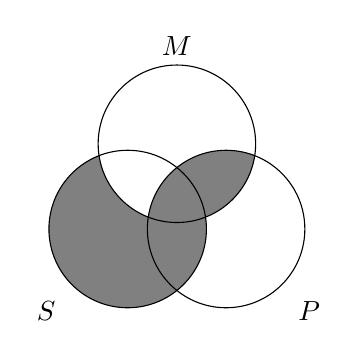
\begin{tikzpicture}
\def\firstcircle{(0,0) circle (1cm)}
\def\secondcircle{(60:1.25cm) circle (1cm)}
\def\thirdcircle{(0:1.25cm) circle (1cm)}

\begin{scope} 
\clip \thirdcircle;
\fill[gray] \secondcircle;
\end{scope}

\begin{scope}[even odd rule] % Shade P without M
\clip \secondcircle (-1,-1) rectangle (2,2);
\fill[gray] \firstcircle;
\end{scope}

\draw \firstcircle node[outer sep=.8cm, below left] {$S$};
\draw \secondcircle node [outer sep=1cm, above] {$M$};
\draw \thirdcircle node [outer sep=.8cm, below right] {$P$};
\end{tikzpicture}
\end{center}

This means you can't assume an argument is invalid because it has a false conclusion. The reverse is also true. You can't assume an argument is valid just because it has a true conclusion. Consider this 

\begin{quotation}  All cats are animals, and some animals are dogs. Therefore no dogs are cats. \end{quotation}

Makes sense, right? Everything is true. But the argument isn't valid. The premises aren't making the conclusion true. Other arguments with the same form have true premises and a false conclusion. Like this one.

\begin{quotation}All chihuahuas are animals, and some animals are dogs. Therefore, no dogs are chihuahuas.\end{quotation}

Really, the arguments in both these passages have the same form: AEE-IV: 

\begin{earg}
\item[P$_1$:] All $P$ are $M$.
\item[P$_2$:] Some $M$ are $S$.
\vspace{-.5em}
\item [] \rule{0.2\linewidth}{.5pt} 
\item[C:] No $S$ are $P$.
\end{earg} 

This in an invalid form, and it remains invalid whether the $P$ stands for cats or chihuahuas. You can see this in the Venn diagram:

\begin{center}
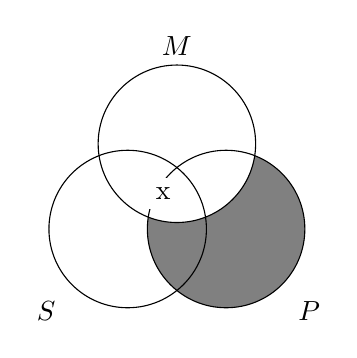
\begin{tikzpicture}
\def\firstcircle{(0,0) circle (1cm)}
\def\secondcircle{(60:1.25cm) circle (1cm)}
\def\thirdcircle{(0:1.25cm) circle (1cm)}

\begin{scope}[even odd rule] % Shade P without M
\clip \secondcircle (-1,-1) rectangle (2.5,2);
\fill[gray] \thirdcircle;
\end{scope}

\draw \firstcircle node[outer sep=.8cm, below left] {$S$};
\draw \secondcircle node [outer sep=1cm, above] {$M$};
\draw \thirdcircle node [outer sep=.8cm, below right] {$P$}
	node[xshift=-.8cm, yshift=.45cm, fill=white](6){x};
\end{tikzpicture}
\end{center}

All these examples bring out an important fact about the kind of logic we are doing in this chapter and the last one: this is \emph{formal} logic. As we discussed on page \pageref{def:Formal_logic} formal logic is a way of making our investigation content neutral. By using variables for terms instead of noun phrases in English we can show that certain ways of arguing are good or bad regardless of the topic being argued about. \iflabelexists{part:formal_logic}{This method will be extended in Chapters \ref{chap:SL} and \ref{chap:QL}, when we introduce our full formal languages SL and QL. } 
{Parts \iflabelexists{part:cat_logic}{This method will be extended in Part \ref{part:sent_logic}, when we introduce the full formal language SL} 
{}}


The examples above also show us another way of proving that an argument given in English is invalid, called the counterexample method. As we have just seen, if you are given an argument in English with, say, false premises and a false conclusion, you cannot determine immediately whether the argument is valid. However, we can look at arguments that have the same form, and use them to see whether the argument is valid. If we can find an argument that has the exact same form as a given argument but has true premises and a false conclusion, then we know the argument is invalid. We just did that with the AEE-IV argument above. We were given an argument with true premises and a true conclusion involving cats, dogs, and animals. We were able to show this argument invalid by finding an argument with the same form that has true premises and a false conclusion, this time involving chihuahuas, dogs, and animals. 


\newglossaryentry{counterexample method}
{
name=counterexample method,
description={A method for determining whether an argument with ordinary English words for terms is valid. One consistently substitutes other English terms for the terms in the given argument to see whether one can find an argument with the same form that has true premises and a false conclusion.}
}

More precisely, we can define the \textsc{\gls{counterexample method}} \label{def:counter_example_method} as a method for determining if an argument with ordinary English words for terms is valid, where one consistently substitutes other English terms for the terms in the given argument to see if one can find an argument with the same form that has true premises and a false conclusion. Let's run through a couple more examples to see how this works. 

First consider this argument in English:

\begin{quotation}
\noindent  All tablet computers are computers. We know this because a computer is a kind of machine, and some machines are not tablet computers. 
\end{quotation}

Every statement in this argument is true, but it doesn't seem right. The premises don't really relate to the conclusion. That means you can probably find an argument with the same form that has true premises and a false conclusion. Let's start by putting the argument in canonical form. Notice that the English passage had the conclusion first. 

\begin{earg} 
\item[P$_1$:] All computers are machines.
\item[P$_2$:] Some machines are not tablet computers.
\vspace{-.5em} 
 \item [] \rule{0.4\linewidth}{.5pt} 
\item[C:] All tablet computers are computers.
 \end{earg}

Let's find substitutes for ``machines,'' ``computers,'' and ``tablet computers'' that will give us true premises and a false conclusion. It is easiest to work with really common sense categories, like ``dog'' and ``cat.'' It is also easiest to start with a false conclusion and then try to find a middle term that will give you true premises. ``All dogs are cats'' is a nice false conclusion to start with:  

\begin{earg} 
\item[P$_1$:] All cats are $M$.
\item[P$_2$:] Some $M$ are not dogs. 
\vspace{-.5em} 
 \item [] \rule{0.3\linewidth}{.5pt} 
\item[C:] All dogs are cats.
 \end{earg}

So what can we substitute for $M$ (which used to be ``machines'') that will make P$_1$ and P$_2$ true? ``Animals'' works fine.

\begin{earg} 
\item[P$_1$:] All cats are animals.
\item[P$_2$:] Some animals are not dogs. 
\vspace{-.5em} 
 \item [] \rule{0.3\linewidth}{.5pt} 
\item[C:] All dogs are cats.
 \end{earg}

There you have it: a counterexample that shows the argument invalid. Let's try another one. 

\begin{quotation}
Some diseases are viral, therefore some things caused by bacteria are not things that are caused by viruses, because all diseases are bacterial.
\end{quotation}

This will take a bit more unpacking. You can see from the indicator words that the conclusion is in the middle. We also have to fix ``viral'' and ``things that are caused by viruses'' so they match, and the same is true for ``bacterial'' and ``things that are caused by bacteria.'' Once we have the sentences in canonical form, the argument will look like this:

\begin{earg} 
\item[P$_1$:] Some diseases are things caused by viruses.
\item[P$_2$:] All diseases are things causes by bacteria.
\vspace{-.5em} 
 \item [] \rule{0.7\linewidth}{.5pt} 
\item[C:] Some things caused by bacteria are not things caused by viruses.
 \end{earg}

Once you manage to think through the complicated wording here, you can see that P$_1$ and the conclusion are true. Some diseases come from viruses, and not everything that comes from a bacteria comes from a virus. But P$_2$ is false. All diseases are not caused by bacteria. In fact, P$_1$ contradicts P$_2$. But none of this is enough to show the argument is invalid. To do that, we need to find an argument with the same form that has true premises and a false conclusion. 

Let's go back to the simple categories: ``dogs,'' ``animals,'' etc. We need a false conclusion. Let's go with ``Some dogs are not animals.'' 

\begin{earg} 
\item[P$_1$:] Some $M$ are dogs.
\item[P$_2$:] All $M$ are animals.
\vspace{-.5em} 
 \item [] \rule{0.3\linewidth}{.5pt} 
\item[C:] Some dogs are not animals.
 \end{earg}

We need a middle term that will make the premises true. It needs to be a class that is more general than ``dogs'' but more narrow than ``animals.'' ``Mammals'' is a good standby here.

\begin{earg} 
\item[P$_1$:] Some mammals are dogs.
\item[P$_2$:] All mammals are animals.
\vspace{-.5em} 
 \item [] \rule{0.3\linewidth}{.5pt} 
\item[C:] Some dogs are not animals.
 \end{earg}

And again we have it, a counterexample to the given syllogism. 

\practiceproblems

\noindent\problempart Each of the following arguments are invalid. Prove that they are invalid by providing a counterexample that has the same form, but true premises and a false conclusion. 
\begin{longtabu}{p{.1\linewidth}p{.9\linewidth}} 
\textbf{Example}: & No pants are shirts, and no shirts are dresses, so some pants are not dresses. \\ 
\textbf{Answer}: & No dogs are reptiles, and no reptiles are mammals, so some dogs are not mammals.   \\ 
\end{longtabu} 

%\begin{earg} 
%\item[P$_1$:] No $P$ are $M$
%\item[P$_2$:] No $M$ are $S$
%\vspace{-.5em} 
% \item [] \rule{0.6\linewidth}{.5pt} 
%\item[C:] Some $S$ are not $P$
% \end{earg}
% EEO-IV Invalid Conclusion First 
% 



\begin{exercises} 

\item Some mammals are animals, and some dogs are mammals. Therefore, all dogs are animals.  

\answer{
\begin{longtabu}{X[1,l,p]X[1,l,p]}
\begin{earg} 
\item[P$_1$:] Some $M$ are $P$
\item[P$_2$:] Some $S$ are $M$
\vspace{-.5em} 
 \item [] \rule{0.6\linewidth}{.5pt} 
\item[C:] All $S$ are $P$
 \end{earg}
 
& 
\begin{earg*}
\item  Some mammals are chihuahuas 
\item Some dogs are mammals
\itemc All dogs are chihuahuas
\end{earg*}
\end{longtabu}
}
 
\item Some evergreens are not spruces, and all spruces are trees. Therefore some trees are not evergreens.

\answer{
\begin{longtabu}{X[1,l,p]X[1,l,p]}

\begin{earg} 
\item[P$_1$:] Some $P$ are not $M$
\item[P$_2$:] All $M$ are $S$
\vspace{-.5em} 
 \item [] \rule{0.6\linewidth}{.5pt} 
\item[C:] Some $S$ are not $P$
 \end{earg}
&
 \begin{earg*}
\item Some plants are not spruces
\item All spruces are trees. 
\itemc Some trees are not plants.
\end{earg*}
\end{longtabu}
}

\item No wild animals are completely safe to be around, and some pigs are not completely safe to be around. Therefore some pigs are wild. 
\answer{
\begin{longtabu}{X[1,l,p]X[2,l,p]}

\begin{earg} 
\item[P$_1$:] No $P$ are $M$
\item[P$_2$:] Some $S$ are not $M$
\vspace{-.5em} 
 \item [] \rule{0.6\linewidth}{.5pt} 
\item[C:] Some $S$ are $P$
 \end{earg}
&
\begin{earg*} 
\item No explosives are completely safe to be around
\item Some pigs are not completely safe to be around. 
\itemc Some pigs are explosives. 
\end{earg*} 
\end{longtabu}
} 

\item Some sodas are clear, and some healthy drinks are clear. Therefore no sodas are healthy.
\answer{
\begin{longtabu}{X[1,l,p]X[1,l,p]}
\begin{earg} 
\item[P$_1$:] Some $P$ are $M$
\item[P$_2$:] Some $S$ are $M$
\vspace{-.5em} 
 \item [] \rule{0.6\linewidth}{.5pt} 
\item[C:] No $S$ are $P$
 \end{earg}
 & 
\begin{earg*}
\item Some beverages are clear
\item Some healthy drinks are clear.
\itemc No beverages are healthy. 
\end{earg*}
\end{longtabu}
}

\item No hamburgers are rocks, no igneous rocks are hamburgers. Therefore all igneous rocks are rocks.
\answer{
\begin{longtabu}{X[1,l,p]X[1,l,p]}

\begin{earg} 
\item[P$_1$:] No $M$ are $P$
\item[P$_2$:] No $S$ are $M$
\vspace{-.5em} 
 \item [] \rule{0.6\linewidth}{.5pt} 
\item[C:] All $S$ are $P$
 \end{earg}
&
\begin{earg*}
\item No hamburgers are cats
\item No dogs are hamburgers. 
\itemc All dogs are cats
\end{earg*}
\end{longtabu}
}

\item Some plants are not food, and some foods are vegetables. Therefore some plants are vegetables.
\answer{
\begin{longtabu}{X[1,l,p]X[1,l,p]}

\begin{earg} 
\item[P$_1$:] Some $P$ are not $M$
\item[P$_2$:] Some $M$ are $S$
\vspace{-.5em} 
 \item [] \rule{0.6\linewidth}{.5pt} 
\item[C:] Some $S$ are $P$
 \end{earg}
&
\begin{earg*}
\item Some plants are not food
\item Some foods are animal products. 
\itemc Some plants are animal products
\end{earg*}
\end{longtabu}
}
\item All apartment buildings are buildings, and some buildings are residential buildings. Therefore some residential buildings are not apartment buildings.
\answer{
\begin{longtabu}{X[1,l,p]X[1,l,p]}
\begin{earg} 
\item[P$_1$:] All $P$ are $M$
\item[P$_2$:] Some $M$ are $S$
\vspace{-.5em} 
 \item [] \rule{0.6\linewidth}{.5pt} 
\item[C:] Some $S$ are not $P$
 \end{earg}
 &

\begin{earg*}
\item All dogs are mammals
\item  Some mammals are animals
\itemc Some dogs are not animals. 
\end{earg*}

\end{longtabu}
}

\item No foods are games, and some games are video games. Therefore no video games are food.
\answer{
\begin{longtabu}{X[1,l,p]X[1,l,p]}

\begin{earg} 
\item[P$_1$:] No $P$ are $M$
\item[P$_2$:] Some $M$ are $S$
\vspace{-.5em} 
 \item [] \rule{0.6\linewidth}{.5pt} 
\item[C:] No $S$ are $P$
 \end{earg}

&
\begin{earg*}
\item No mammals are reptiles
\item Some reptiles are pets
\itemc No pets are mammals
\end{earg*}
\end{longtabu}
}
\item Some trucks are rentals, and no cars are trucks. Therefore some cars are rentals.
\answer{
\begin{longtabu}{X[1,l,p]X[1,l,p]}

\begin{earg} 
\item[P$_1$:] Some $M$ are $P$
\item[P$_2$:] No $S$ are $M$
\vspace{-.5em} 
 \item [] \rule{0.6\linewidth}{.5pt} 
\item[C:] Some $S$ are $P$
 \end{earg}

&
\begin{earg*}
\item Some plants are food
\item No cars are plants.
\itemc Some cars are food.  
\end{earg*}
\end{longtabu}
}

\item Some online things are not fun, and some fun things are not video games. Therefore, some video games are online.
\answer{
\begin{longtabu}{X[1,l,p]X[1,l,p]}

\begin{earg} 
\item[P$_1$:] Some $P$ are not $M$
\item[P$_2$:] Some $M$ are not $S$
\vspace{-.5em} 
 \item [] \rule{0.6\linewidth}{.5pt} 
\item[C:] Some $S$ are $P$
 \end{earg}
&
\begin{earg*}
\item Some foods are not fun
\item Some fun things are not video games.
\vspace{-1em} 
\itemc Some video games are food.
\end{earg*}
\end{longtabu}
}
\end{exercises} 

\noindent\problempart Each of the following arguments are invalid. Prove that they are invalid by providing a counterexample that has the same form, but true premises and a false conclusion. 

\begin{exercises}      
 

\item All cars are machines, and all vehicles are machines. Therefore all cars are vehicles.  
\answer{
\begin{earg} 
\item[P$_1$:] All $P$ are $M$
\item[P$_2$:] All $S$ are $M$
\vspace{-.5em} 
 \item [] \rule{0.6\linewidth}{.5pt} 
\item[C:] All $S$ are $P$
 \end{earg}
 AAA-II Invalid 
 
 All cars are machines and all trucks are machines. Therefore all cars are trucks.}
 

\item Some black animals are panthers. No panthers are sheep. Therefore some sheep are black. 

\answer{Some carnivorous animals are panthers. No panthers are sheep. Some sheep are carnivorous.
\begin{earg} 
\item[P$_1$:] Some $P$ are $M$
\item[P$_2$:] No $M$ are $S$
\vspace{-.5em} 
 \item [] \rule{0.6\linewidth}{.5pt} 
\item[C:] Some $S$ are $P$
 \end{earg}
 IEI-IV Invalid }


\item Some paper money is not counterfeit, and some counterfeit monies are quarters. Therefore no quarters are paper money.
\answer{
\begin{earg}
\item[P$_1$:] Some $P$ are not $M$
\item[P$_2$:] Some $M$ are $S$
\vspace{-.5em} 
 \item [] \rule{0.6\linewidth}{.5pt} 
\item[C:] No $S$ are $P$
 \end{earg}
 OIE-IV Invalid 
 
Some legal tender is not counterfeit, and some counterfeit monies are quarters. Therefore no quarters are legal tender.}
 
\item Some spacecraft are man-made, and no comets are man-made. Therefore some comets are not spacecraft.
\answer{
\begin{earg} 
\item[P$_1$:] Some $P$ are $M$
\item[P$_2$:] No $S$ are $M$
\vspace{-.5em} 
 \item [] \rule{0.6\linewidth}{.5pt} 
\item[C:] Some $S$ are not $P$
 \end{earg}
 IEO-II Invalid 
: Some things made of rock and ice are man-made, and no comets are man-made. Therefore some comets are not things made of rock and ice}
 
 
\item No planets are stars, and no planets are fusion reactions. Therefore all stars are fusion reactions.

\answer{No planets are starts and no planets are asteroids. Therefore all stars are asteroids. 
\begin{earg} 
\item[P$_1$:] No $M$ are $P$
\item[P$_2$:] No $M$ are $S$
\vspace{-.5em} 
 \item [] \rule{0.6\linewidth}{.5pt} 
\item[C:] All $S$ are $P$
 \end{earg}
 EEA-III Invalid }
 
\item All straight lines are lines, and no straight lines are curved lines. Therefore, all curved lines are lines.

\answer{All straight lines are lines, and no cows are curved lines. Therefore, all cows are lines.
\begin{earg} 
\item[P$_1$:] All $M$ are $P$
\item[P$_2$:] No $M$ are $S$
\vspace{-.5em} 
 \item [] \rule{0.6\linewidth}{.5pt} 
\item[C:] All $S$ are $P$
 \end{earg}
 AEA-III Invalid }
 
\item Some physical objects are not writing implements, and all pencils are writing implements. Therefore, all pencils are physical objects.

\answer{Some foods are not writing implements, and all pencils are writing implements. Therefore, all pencils are food.

\begin{earg} 
\item[P$_1$:] Some $P$ are not $M$
\item[P$_2$:] All $S$ are $M$
\vspace{-.5em} 
 \item [] \rule{0.6\linewidth}{.5pt} 
\item[C:] All $S$ are $P$
 \end{earg}
 OAA-II Invalid }
 
\item No traumatic memories are pleasant, but some memories are traumatic. Therefore, some memories are pleasant.

\answer{No chihuahuas are cats, but some dogs are chihuahuas. Therefore, some dogs are cats
\begin{earg} 
\item[P$_1$:] No $M$ are $P$
\item[P$_2$:] Some $S$ are $M$
\vspace{-.5em} 
 \item [] \rule{0.6\linewidth}{.5pt} 
\item[C:] Some $S$ are $P$
 \end{earg}
 EII-I Invalid }

\item Some farms are for-profit enterprises, and all munitions factories are for-profit enterprises. Therefore, no munitions factories are farms.

\answer{Some mammals are animals, and all dogs are animals, so no dogs are mammals 
\begin{earg} 
\item[P$_1$:] Some $P$ are $M$
\item[P$_2$:] All $S$ are $M$
\vspace{-.5em} 
 \item [] \rule{0.6\linewidth}{.5pt} 
\item[C:] No $S$ are $P$
 \end{earg}
 IAE-II Invalid }

\item No parasites are western brook lampreys, and all western brook lampreys are lampreys. Therefore some lampreys are parasitic. 

\answer{
\begin{earg} 
\item[P$_1$:] No $P$ are $M$
\item[P$_2$:] All $M$ are $S$
\vspace{-.5em} 
 \item [] \rule{0.6\linewidth}{.5pt} 
\item[C:] Some $S$ are $P$
 \end{earg}
 EAI-IV }
   
         
\end{exercises}

% *******************************************
% *               Ordinary Language Arguments             *
% *******************************************

\section{Ordinary Language Arguments}

In the last section we saw that arguments in ordinary language can throw us off because our knowledge of the truth or falsity of the statements in them can cloud our perception of the validity of the argument. Now we are going to look at ways we might need to transform ordinary language arguments in order to put them in standard form (see p. \pageref{standard_form_for_an_Aristotelian_syllogism}) and use our evaluative tools.  
%%%%%%%%%% Basic Transformations in to LSE  %%%%%%%%

\subsection{Basic Transformations into Logically Structured English}

Arguments are composed of statements, so all of the guidelines we discussed for putting ordinary English statements into logically structured English in Section \ref{sec:transformation} apply here. Also, as you saw in the exercises in Section \ref{sec:form_mood_figure}, we need to be aware that the conclusion of an ordinary language argument can occur anywhere in the passage. Consider this argument

\begin{quotation}
\noindent Every single penguin in the world is a bird. Therefore, at least one bird in the world is not a person, because not one person is a penguin.
\end{quotation}

The indicator words let us know the conclusion is the sentence in the middle of this passage, ``At least one bird in the world is not a person.'' The quantifier in this sentence is nonstandard. As we saw on page \pageref{subsec:nonstandard_quantifiers} ``at least one'' should be changed to ``some.'' That would give us ``Some birds are not people'' for the conclusion. Similar changes need to be made to the two premises. Thus the argument and translation key look like this: 

\begin{tabu}{{X[1,l,p]X[1,l,p]}}


\begin{ekey}
\item[$S$:] Birds
\item[$M$:] Penguins
\item[$P$:] People
\end{ekey}

&

\begin{earg}
\item[P$_1$:] No $P$ are $M$. 
\item[P$_2$:] All $M$ are $S$.
\vspace{-.5em}
\item [] \rule{0.4\linewidth}{.5pt} 
\item[C:] Some $S$ are not $P$.
\end{earg} 

\end{tabu}

Now that we have it in this form, we can see that it is the argument Fesapo (EAO-4), which is valid if you add the premise that some penguins exist.

Another issue that can come up in ordinary language arguments is the use of synonyms. Consider another argument about penguins:

\begin{quotation}
\noindent No Ad\'{e}lie penguins can fly, because all members of \emph{Pygoscelis adeliae} are members of the family Sphenisciformes, and no Sphenisciformes can fly.
\end{quotation}

You might think this argument can't be a proper syllogism, because it has four terms in it: Ad\'{e}lie penguins, \emph{Pygoscelis adeliae}, Sphenisciformes, and things that can fly. However, a quick trip to Wikipedia can confirm that \emph{Pygoscelis adeliae} is just the scientific name from the Ad\'{e}lie penguin, and for that matter ``Sphenisciformes'' are just penguins. So really, the argument just has three terms, and there is no problem representing the argument  like this:

\begin{tabu}{{X[1,l,p]X[1,l,p]}}


\begin{ekey}
\item[$S$:] Ad\'{e}lie penguins
\item[$M$:] Penguins
\item[$P$:] Things that can fly 
\end{ekey}

&

\begin{earg}
\item[P$_1$:]  No $M$ are $P$.
\item[P$_2$:] All $S$ are $M$.
\vspace{-.5em}
\item [] \rule{0.4\linewidth}{.5pt} 
\item[C:] No $S$ are $P$.
\end{earg} 

\end{tabu}

And this is our good friend Celarent (EAE-1). 

Generally speaking, arguments involving different names for the same person can work the same way as synonyms. Consider this argument:

\begin{quotation}
\noindent Bertrand Russell was a philosopher. We know this because Mr. Russell was a logician, and all logicians are philosophers. 
\end{quotation}

``Bertrand Russell'' and ``Mr. Russell'' are names for the same person, so we can represent them using the same variable. Back on page \pageref{subsec:singular_propositions} we learned that names for individuals need to be transformed into classes using phrases like ``objects identical with \ldots'' or ``people identical with \ldots.''  Thus the argument turns out to be Celarent's best friend, Barbara (AAA-I):

\begin{tabu}{{X[1.25,l,p]X[1,l,p]}}


\begin{ekey}
\item[$S$:] People identical with Bertrand Russell
\item[$M$:] Logicians
\item[$P$:] Philosophers 
\end{ekey}

&

\begin{earg}
\item[P$_1$:]  All $M$ are $P$.
\item[P$_2$:] All $S$ are $M$.
\vspace{-.5em}
\item [] \rule{0.4\linewidth}{.5pt} 
\item[C:] All $S$ are $P$.
\end{earg} 

\end{tabu}

Merging proper nouns into one variable doesn't always work the way merging synonyms does, however. Sometimes exchanging one name with another can change the truth value of a sentence, even when the two names refer to the same person. Any comic book fan will tell you that the sentence ``J. Jonah Jameson hates Spider-Man'' is true. Also, ``Peter Parker'' and ``Spider-Man'' refer to the same person. However ``J. Jonah Jameson hates Peter Parker'' is false. These situations are called ``intentional contexts.'' We won't be dealing with them in this textbook, but you should be aware that they exist. 

Another thing to be aware of when you assign variables to terms is that often you will need to find the right general category that will allow your terms to hook up with each other. \label{finding_general_terms} Consider this argument.

\begin{quotation}
Bertrand Russell did not believe in God. I know this because Mr. Russell was not a Christian, and all Christians believe in God
\end{quotation}

Here again we need to use one variable for both ``Bertrand Russell'' and ``Mr. Russell.'' But we also have to change the verb phrase ``believes in God'' into a predicate term (see page \pageref{subsec:nonstandard_verbs}). The main trick here is to transform the verb phrase ``believes in God'' and the singular terms referring to Bertrand Russell in a way that will match. The trick is to use the word ``people'' each time. ``Believes in God'' becomes ``people who believe in God,'' and the two names for Bertrand Russell need to become ``people identical with Bertrand Russell.'' By including the word ``people'' in each case, we ensure that the terms will be comparable. 
 
\begin{tabu}{{X[2,l,p]X[1,l,p]}}

\begin{ekey}
\item[$S$:] People identical to Bertrand Russell
\item[$M$:] Christians
\item[$P$:] People who believe in God
\end{ekey}

&

\begin{earg}
\item[P$_1$:] All $M$ are $P$.
\item[P$_2$:] No $S$ are $M$.
\vspace{-.5em}
\item [] \rule{0.5\linewidth}{.5pt} 
\item[C:] No $S$ are $P$.
\end{earg} 

\end{tabu}

The argument here is AEE-1, which is invalid. It violates rule 2, because $P$ is distributed in the conclusion, but not the premises. More informally, we can say that just because Russell wasn't a Christian doesn't mean he was an atheist or an agnostic. (In fact, Russell said that he was an atheist in some ways, and an agnostic in others, but this argument doesn't show that.) 

%%%%%%%%%%%% Complement classes, etc. %%%%

\subsection{Complement Classes, Obversion, and Contraposition}

In the last subsection, we saw that we can represent synonyms using the same variable, thus reducing the number of terms in an argument down to the three terms required for an Aristotelian syllogism. Something similar can be done when you have terms that are complements of other terms. Back on page \pageref{def:Complement} we said that the complement of a class was the class of things that are not in the original class. So the complement of the class ``penguins'' is everything that is not a penguin. Sometimes, if you have an argument with more than three terms, you can reduce the number of terms down to three, because some of the terms are complements of each other, like ``penguins'' and ``non-penguins.''

 Consider the following argument, which talks about the stoics, an ancient philosophical school and pioneers in logical thinking. \nix{[insert historical sidebar ref]}

\begin{quotation}
No stoics are non-logicians, and all non-philosophers are non-stoics. Therefore all logicians are philosophers.
\end{quotation}

This argument has six terms: stoics, logicians, philosophers, non-stoics, non-logicians, and non-philosophers. Since the second three are all complements of the first, we should be able to reduce the number of terms to three. Once we do this, we might find that the argument is valid---it looks like it might be Barbara. We can begin by assigning $S$, $M$, and $P$ to the terms ``stoics,'' ``logicians,'' and ``philosophers.'' We can then represent the other six terms as non-$S$, non-$M$, and non-$P$. 


\begin{tabu}{{X[1,l,p]X[1,l,p]}}

\begin{ekey}
\item[$S$:] Logicians
\item[$M$:] Stoics
\item[$P$:] Philosophers
\end{ekey}

&

\begin{earg}
\item[P$_1$:]  No $M$ are non-$P$.
\item[P$_2$:] All non-$S$ are non-$M$.
\vspace{-.5em}
\item [] \rule{0.6\linewidth}{.5pt} 
\item[C:] All $S$ are $P$.
\end{earg} 

\end{tabu}

The argument still has six terms, so we can't evaluate it as is. However, we can get rid of three of these terms. The secret is to apply two of the transformation tools we learned about in Section \ref{sec:conv_obv_cont}, obversion and contraposition. In that section, we saw that there were different ways you could alter categorical statements that would sometimes yield a logically equivalent statement. Two of those methods---obversion and contraposition---involved taking the complements of existing terms. In the cases where these transformations yield logically equivalent terms, we can use them to change the premises of an argument into statements that lack the terms we want to get rid of. 

In obversion, you change the quality of a sentence---switch it from affirmative to negative or vice versa---and then replace the predicate term with its complement. This process always yields a logically equivalent statement, so we can always use it. Applying obversion to the first premise of the argument above allows us to eliminate the term non-$P$.  

\begin{earg}
\item[P$_1$:]  All $M$ are $P$.
\item[P$_2$:] All non-$S$ are non-$M$.
\vspace{-.5em}
\item [] \rule{0.25\linewidth}{.5pt} 
\item[C:] All $S$ are $P$.
\end{earg} 

We can also use contraposition to eliminate terms, but here we must be more careful. Contraposition only yields logically equivalent statements when it is applied to mood-A or mood-O statements. Fortunately, Premise 2 is a mood-A statement, so we can change the argument to look like this:

\begin{earg}
\item[P$_1$:]  All $M$ are $P$.
\item[P$_2$:] All $M$ are $S$.
\vspace{-.5em}
\item [] \rule{0.2\linewidth}{.5pt} 
\item[C:] All $S$ are $P$.
\end{earg} 

And now the argument only has three terms, and we can evaluate it. As you can see it is not Barbara at all, but one of her unnamed evil step-sisters, AAA-3. Again, remember not to use contraposition on mood-E or mood-I statements. You can use obversion on any statement, but contraposition only works on mood A or mood O.  

Ordinary English has other prefixes besides ``non-'' to denote the complements of classes. ``Un-'' is the most common prefix, but English also uses ``in-,'' ``dis-,'' and ``a-.'' These can be handled the same way ``non-'' is. Consider,

\begin{quotation}
All dogs in the park must be leashed. Some unleashed pets in the park are cats. Therefore, some cats in the park are not dogs.
\end{quotation}

To make this argument work, we need to get the predicate of the major premise to match the subject of the minor premise. The first step is just turning the verb phrase ``must be leashed'' into a noun phrase that matches ``unleashed pets.'' We also should use the qualification ``in the park'' consistently across the terms. 

\begin{tabu}{{X[1,l,p]X[1,l,p]}}

\begin{ekey}
\item[$S$:] Cats in the park
\item[$M$:] Leashed pets in the park
\item[$P$:] Dogs in the park 
\end{ekey}

&

\begin{earg}
\item[P$_1$:]  All $P$ are $M$.
\item[P$_2$:] Some non-$M$ are $S$.
\vspace{-.5em}
\item [] \rule{0.6\linewidth}{.5pt} 
\item[C:] Some $S$ are not $P$.
\end{earg} 

\end{tabu}

Now the trick is to get the terms $M$ and non-$M$ to match. We could try to transform the second premise, but that won't do us any good. It is an E statement, so we can't use contraposition, and obversion won't change the subject term. 

Instead of changing the ``non-$M$'' to ``$M$'' in the second premise, we need to change the ``$M$'' to ``non-$M$'' in the first premise. We can do this using obversion, which works on statements in any mood.  

\begin{earg}
\item[P$_1$:]  No $P$ are non-$M$.
\item[P$_2$:] Some non-$M$ are $S$.
\vspace{-.5em}
\item [] \rule{0.2\linewidth}{.5pt} 
\item[C:] Some $S$ are not $P$.
\end{earg} 

And now we can see that the argument is Fresison (EIO-4), which is valid.


\practiceproblems

\noindent \problempart The following arguments are given with variables for the terms. Use obversion and contraposition to reduce the number of terms to three. State which operations you are using on which statements, and give the resulting syllogism in canonical form. Finally, use Venn diagrams to evaluate the argument.

\begin{longtabu}{p{.1\linewidth}p{.3\linewidth}p{.6\linewidth}}

\textbf{Example}: & \multicolumn{2}{p{.9\linewidth}}{No $M$ are $P$, and all non-$M$ are non-$S$. Therefore all $S$ are non-$P$.}\\

\textbf{Answer}: & \multicolumn{2}{p{.9\linewidth}}{Use contraposition on the minor premise and obversion on the conclusion to get the following} \\ 
 &
\begin{earg} 
\item[P$_1$:] No $M$ are $P$.
\item[P$_2$:] All $S$ are $M$.
\vspace{-.5em} 
 \item [] \rule{0.4\linewidth}{.5pt} 
\item[C:] No $S$ are $P$.
 \end{earg} 

Valid, Celartent (EAE-1)

&


\vspace{-.75cm}
\hspace{-1cm}

\begin{center}
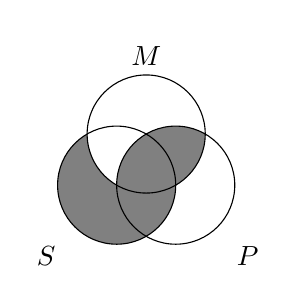
\begin{tikzpicture}
\def\firstcircle{(0,0) circle (.75cm)}
\def\secondcircle{(60:.75cm) circle (.75cm)}
\def\thirdcircle{(0:.75cm) circle (.75cm)}

\begin{scope} 
\clip \thirdcircle;
\fill[gray] \secondcircle;
\end{scope}

\begin{scope}[even odd rule] % Shade P without M
\clip \secondcircle (-1,-1) rectangle (2,2);
\fill[gray] \firstcircle;
\end{scope}

\draw \firstcircle node[outer sep=.66cm, below left] {$S$};
\draw \secondcircle node [outer sep=.75cm, above] {$M$};
\draw \thirdcircle node [outer sep=.66cm, below right] {$P$};
\end{tikzpicture}
\end{center}
\end{longtabu} 


\begin{exercises} 
\item No $P$ are $M$, and all non-$S$ are non-$M$. Therefore some $S$ are $P$. 

\answer{

Use contraposition on the minor premise to get the following

\begin{longtabu}{X[1,l,m]X[1,l,m]} 

\begin{earg} 
\item[P$_1$:] No $P$ are $M$
\item[P$_2$:] All $M$ are $S$
\vspace{-.5em} 
 \item [] \rule{0.6\linewidth}{.5pt} 
\item[C:] Some $S$ are $P$
 \end{earg}
 EAI-IV Invalid 

&

\begin{venns}
\shadeintersectred{\middlecircle}{\predicatecircle}
\shadecomplementred{\middlecircle}{\middlesquare}{\subjectcircle}
\drawsubsyl
\drawmidsyl
\drawpredsyl
\end{venns}

\end{longtabu}
}


\item No $P$ are $M$, and all $S$ are $M$. Therefore all $S$ are non-$P$.
\answer{
Take the obverse of the conclusion to get:


\begin{longtabu}{X[1,l,m]X[1,l,m]} 

\begin{earg} 
\item[P$_1$:] No $P$ are $M$
\item[P$_2$:] All $S$ are $M$
\vspace{-.5em} 
 \item [] \rule{0.6\linewidth}{.5pt} 
\item[C:] No $S$ are $P$
 \end{earg} 
Cesare (EAE-II) (Valid) 


&
\begin{venns}
\shadeintersectred{\middlecircle}{\predicatecircle}
\shadecomplementred{\subjectcircle}{\subjectsquare}{\middlecircle}
\drawsubsyl
\drawmidsyl
\drawpredsyl
\end{venns}
\end{longtabu}

}
\item No $M$ are $P$, and some $S$ are $M$. Therefore some non-$P$ are not non-$S$.

\answer{
Take the contrapositive of the conclusion to get


\begin{longtabu}{X[1,l,m]X[1,l,m]} 

\begin{earg} 
\item[P$_1$:] No $M$ are $P$
\item[P$_2$:] Some $S$ are $M$
\vspace{-.5em} 
 \item [] \rule{0.6\linewidth}{.5pt} 
\item[C:] Some $S$ are not $P$
 \end{earg} 
Ferio (EIO-I) (valid) 
 
&
\begin{venns}
\shadeintersectred{\middlecircle}{\predicatecircle}
\someexistfive
\drawsubsyl
\drawmidsyl
\drawpredsyl
\end{venns}
\end{longtabu}
}
\item All non-$P$ are non-$M$, and some $S$ are $M$. Therefore all $S$ are $P$. 

\answer{
 Perform contraposition on the major premise to get

\begin{longtabu}{X[1,l,m]X[1,l,m]} 

\begin{earg} 
\item[P$_1$:] All $M$ are $P$
\item[P$_2$:] Some $S$ are $M$
\vspace{-.5em} 
 \item [] \rule{0.6\linewidth}{.5pt} 
\item[C:] All $S$ are $P$
 \end{earg}
 AIA-I Invalid 
 
&
\begin{venns}
\shadecomplementred{\middlecircle}{\middlesquare}{\predicatecircle}
\someexistseven
\drawsubsyl
\drawmidsyl
\drawpredsyl
\end{venns}
\end{longtabu}
}
\item All non-$M$ are non-$P$, and no $S$ are $M$. Therefore no $S$ are $P$. 
\answer{
Perform contraposition on the major premise to get

\begin{longtabu}{X[1,l,m]X[1,l,m]} 

\begin{earg} 
\item[P$_1$:] All $P$ are $M$
\item[P$_2$:] No $S$ are $M$
\vspace{-.5em} 
 \item [] \rule{0.6\linewidth}{.5pt} 
\item[C:] No $S$ are $P$
 \end{earg} 
Camestres (AEE-II) (valid) 
%
% 
&
\begin{venns}
\shadecomplementred{\predicatecircle}{\predicatesquare}{\middlecircle}
\shadeintersectred{\subjectcircle}{\middlecircle}
\drawsubsyl
\drawmidsyl
\drawpredsyl
\end{venns}
\end{longtabu}
}
\item All $P$ are $M$, and all $S$ are non-$M$. Also, some $S$ exist. Therefore, some $S$ are not $P$.
\answer{
Perform obversion on the minor premise to get

\begin{longtabu}{X[1,l,m]X[1,l,m]} 

\begin{earg*}
\item All $P$ are $M$
\item No $S$ are $M$
\item Some $S$ exist.
\itemc Some $S$ are not $P$
\end{earg*}

AEO-IV (conditionally valid) 

&
\begin{venns}
\shadecomplementred{\predicatecircle}{\predicatesquare}{\middlecircle}
\shadeintersectred{\subjectcircle}{\middlecircle}
\someexistone
\drawsubsyl
\drawmidsyl
\drawpredsyl
\end{venns}
\end{longtabu}
}
\item Some $P$ are not non-$M$. All non-$M$ are non-$S$. Some $S$ exist. Therefore some $S$ are $P$. 
\answer{
perform obversion on the major premise and contraposition on the minor premise  

\begin{longtabu}{X[1,l,m]X[1,l,m]} 

\begin{earg} 
\item[P$_1$:] Some $P$ are $M$
\item[P$_2$:] All $S$ are $M$
\item[P$_3$:] Some $S$ exist. 
\vspace{-.5em} 
 \item [] \rule{0.6\linewidth}{.5pt} 
\item[C:] Some $S$ are $P$
 \end{earg}
 IAI-II Invalid 

&
\begin{venns}
\SaMred
\drawsubsyl
\drawmidsyl
\drawpredsyl
\someexistsixseven
\someexistfiveseven
\end{venns}
\end{longtabu}
}

\item All non-$M$ are non-$P$, and all $S$ are non-$M$. Therefore no $S$ are $P$. 
\answer{
Perform contraposition on the major premise and obversion on the minor premise to get: 
\begin{longtabu}{X[1,l,m]X[1,l,m]} 

\begin{earg} 
\item[P$_1$:] All $P$ are $M$
\item[P$_2$:] No $S$ are $M$
\vspace{-.5em} 
 \item [] \rule{0.6\linewidth}{.5pt} 
\item[C:] No $S$ are $P$
 \end{earg} 
Camestres (AEE-II) (valid) 

% 
&
\begin{venns}
\PaMred
\SeMred
\drawsubsyl
\drawmidsyl
\drawpredsyl

\end{venns}
\end{longtabu}
}
\item All $P$ are $M$, and all $M$ are non-$S$. Therefore all $P$ are non-$S$

\answer{
Take the obverse of the minor premise and the conclusion to get:

\begin{longtabu}{X[1,l,m]X[1,l,m]} 
\begin{earg} 
\item[P$_1$:] All $P$ are $M$
\item[P$_2$:] No $M$ are $S$
\vspace{-.5em} 
 \item [] \rule{0.6\linewidth}{.5pt} 
\item[C:] No $S$ are $P$
 \end{earg} 
Calemes (AEE-IV) (valid) 
% 
&
\begin{venns}

\PaMred
\SeMred


\drawsubsyl
\drawmidsyl
\drawpredsyl

\end{venns}
\end{longtabu}
}

\item All $M$ are $P$, and some non-$M$ are not $S$. Therefore some $S$ are not non-$P$. 

 \answer{Convert the minor premise to get ``Some $S$ are not non-$M$.'' Then take the obverse to get ``Some $S$ are $M$.'' Then take the obverse of the conclusion to get:
 
\begin{longtabu}{X[1,l,m]X[1,l,m]} 

\begin{earg} 
\item[P$_1$:] All $M$ are $P$
\item[P$_2$:] Some $S$ are $M$
\vspace{-.5em} 
 \item [] \rule{0.6\linewidth}{.5pt} 
\item[C:] Some $S$ are $P$
 \end{earg} 
Darii (AII-1) (valid) 


%
&
\begin{venns}
\MaPred
\someexistseven
\drawsubsyl
\drawmidsyl
\drawpredsyl

\end{venns}
\end{longtabu}
}
\end{exercises}	
\noindent\problempart The following arguments are given with variables for the terms. Use obversion and contraposition to reduce the number of terms to three. State which operations you are using on which statements, and give the resulting syllogism in canonical form. Finally, use Venn diagrams to evaluate the argument.
\begin{exercises} 

\item All non-$M$ are non-$P$, and no $S$ are $M$. Therefore no $S$ are $P$. 

\answer{
\begin{earg} 
\item[P$_1$:] All $P$ are $M$
\item[P$_2$:] No $S$ are $M$
\vspace{-.5em} 
 \item [] \rule{0.6\linewidth}{.5pt} 
\item[C:] No $S$ are $P$
 \end{earg} 
Camestres (AEE-II) (valid) 
contraposition Major premise }

\item All non-$P$ are non-$M$, and all non-$M$ are non-$S$. Therefore all $S$ are $P$.

\answer{
\begin{earg} 
\item[P$_1$:] All $M$ are $P$
\item[P$_2$:] All $S$ are $M$
\vspace{-.5em} 
 \item [] \rule{0.6\linewidth}{.5pt} 
\item[C:] All $S$ are $P$
 \end{earg} 
   }
         
\item All non-$M$ are non-$P$, and no $M$ are $S$. Also, some $S$ exist. Therefore some $S$ are not $P$. 

\answer{
AEO-IV (conditionally valid) 
contraposition Major premise  
}
 
\item Some $M$ are $P$ and no $M$ are non-$S$. Therefore some $S$ are $P$. 

\answer{
\begin{earg} 
\item[P$_1$:] Some $M$ are $P$
\item[P$_2$:] All $M$ are $S$
\vspace{-.5em} 
 \item [] \rule{0.6\linewidth}{.5pt} 
\item[C:] Some $S$ are $P$
 \end{earg}
 IAI-III Invalid 
obverse Minor premise  
}
 
\item No $P$ are $M$, and all $M$ are non-$S$. Therefore no $S$ are $P$. 

\answer{
\begin{earg} 
\item[P$_1$:] No $P$ are $M$
\item[P$_2$:] No $M$ are $S$
\vspace{-.5em} 
 \item [] \rule{0.6\linewidth}{.5pt} 
\item[C:] No $S$ are $P$
 \end{earg}
 IAA-4 
obv Minor premise  
}
 
\item No $P$ are $M$, and all $S$ are $M$. Also some $S$ exist. Therefore some non-$P$ are not non-$S$. 
\answer{EAO-1I (conditionally valid) 
contraposition Conclusion } 
 
\item All $P$ are $M$, and no $S$ are $M$. Therefore all $S$ are non-$P$.
\answer{
\begin{earg} 
\item[P$_1$:] All $P$ are $M$
\item[P$_2$:] No $S$ are $M$
\vspace{-.5em} 
 \item [] \rule{0.6\linewidth}{.5pt} 
\item[C:] No $S$ are $P$
 \end{earg} 
Camestres (AEE-II) (valid) 
obverse Conclusion  
 obverse Minor premise  
} 
 
\item All $M$ are $P$, and all $M$ are $S$. Also, some $M$ exist. Therefore some $S$ are not non-$P$. 
\answer{
AAI-III (conditionally valid) 
obverse Minor premise  
 obverse Conclusion  }
 
\item All non-$P$ are non-$M$, and some $M$ are not $S$. Also some $M$ exist. Therefore, some non-$P$ are $S$. 

\answer{
\begin{earg} 
\item[P$_1$:] All $M$ are $P$
\item[P$_2$:] Some $M$ are not $S$
Some $M$ exist. 
\vspace{-.5em} 
 \item [] \rule{0.6\linewidth}{.5pt} 
\item[C:] Some $S$ are not $P$
 \end{earg}
 AOO-III Invalid 
 contraposition Conclusion  then obverse Conclusion  
 contraposition major premise
}
 
\item All non-$M$ are non-$P$, and all $M$ are non-$S$. Therefore all $S$ are non-$M$. 

\answer{
\begin{earg} 
\item[P$_1$:] All $P$ are $M$
\item[P$_2$:] No $M$ are $S$
\vspace{-.5em} 
 \item [] \rule{0.6\linewidth}{.5pt} 
\item[C:] No $S$ are $P$
 \end{earg} 
Calemes (AEE-IV) (valid) 
contraposition Major premise  
 obsert  minor premise  
 obverse Conclusion  
}
 
   
\end{exercises}



\noindent \problempart For each inference make a translation key and put the argument in standard form. If you use obversion or contraposition to reduce the number of the terms, make a note of it. Then construct a Venn diagram for it, and determine whether the inference is valid. 

\begin{longtabu}{p{.1\linewidth}p{.5\linewidth}p{.4\linewidth}}
\textbf{Example}: & \multicolumn{2}{p{.9\linewidth}}{No one who studies logic is completely stupid, and some philosophers are not non-logicians. Therefore some philosophers are not completely stupid.} \\
\\
\textbf{Answer}: & $S$: Philosophers \newline
					$M$: Logicians \newline
					$P$: People who are completely stupid \newline 
					Obversion on the minor premise

& 
\vspace{-16pt}
\begin{earg}
\item[P$_1$:] No $M$ are $P$.
\item[P$_2$:] Some $S$ are $M$.
\vspace{-.5em}
\item [] \rule{0.4\linewidth}{.5pt} 
\item[C:] Some $S$ are not $P$.
\end{earg} \\

& 
\vspace{-28pt}
\begin{center}
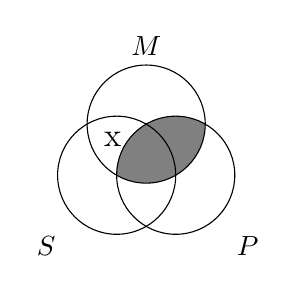
\begin{tikzpicture}
\def\firstcircle{(0,0) circle (.75cm)}
\def\secondcircle{(60:.75cm) circle (.75cm)}
\def\thirdcircle{(0:.75cm) circle (.75cm)}

\begin{scope} %shade overlap between S and M
\clip \thirdcircle;
\fill[gray] \secondcircle;
\end{scope}

\draw \secondcircle node [outer sep=.75cm, above] {$M$};
\draw \thirdcircle node [outer sep=.66cm, below right] {$P$};
\draw \firstcircle node[outer sep=.66cm, below left] {$S$}
	node [xshift=-.05cm, yshift=.45cm](5){\large{x}};
\end{tikzpicture}
\end{center}

& Ferio (EIO-1) \newline Unconditionally valid

\end{longtabu}

%No food is inedible. In fact, all food is edible. Therefore nothing this is inedible is edible. 

\begin{exercises}

\item All of Lorain County is outside of Cuyahoga County, but at least some of Cleveland is in Cuyahoga County. Therefore some of Lorain County is not in Cleveland. 

\answer{

\begin{longtabu}{X[1,l,p]X[1,l,p]}

\begin{ekey}
\item[$S$:] Places in Lorain County 
\item[$M$:] Places in Cuyahoga County
\item[$P$:] Places in Cleveland
\end{ekey}

&

\begin{earg} 
\item[P$_1$:] Some $P$ are $M$
\item[P$_2$:] No $S$ are $M$  %All $S$ are non-$M$
\vspace{-.5em} 
 \item [] \rule{0.6\linewidth}{.5pt} 
\item[C:] Some $S$ are not $P$
 \end{earg} 
IEO-II (Invalid) 

\end{longtabu}
}

\item All Civics are vehicles. After all, any automobile is a vehicle, and a Civic is a kind of car.  

\answer{
\begin{longtabu}{X[1,l,p]X[1,l,p]}

\begin{ekey}
\item[$S$:] Civics
\item[$M$:] Car (or automobile)
\item[$P$:] Vehicle. 
\end{ekey}

&

\begin{earg} 
\item[P$_1$:] All $M$ are $P$
\item[P$_2$:] All $S$ are $M$
\vspace{-.5em} 
 \item [] \rule{0.6\linewidth}{.5pt} 
\item[C:] All $S$ are $P$
 \end{earg} 
Barbara (AAA-I) (valid) 

\end{longtabu}
}

\item Cows are animals. After all, anything that is not an animal is also not a farm animal, and cows are farm animals. 

\answer{
\begin{longtabu}{X[1,l,p]X[1,l,p]}

\begin{ekey}
\item[$S$:] Cows
\item[$M$:] Farm animals
\item[$P$:] Animals
\end{ekey}
 Contrapose major premise.
&

\begin{earg*}
\item All $M$ are $P$
\item All $S$ are $M$
\itemc All $S$ are $P$
\end{earg*}


Barbara (AAA-1) (Valid.)

  \end{longtabu}
} 
         
\item Some digits are fingers, and if something is a digit, then it is a body part. Therefore some body parts are non-fingers. 

\answer{
\begin{longtabu}{X[1,l,p]X[1,l,p]}

\begin{ekey}
\item[$S$:] Body Parts
\item[$M$:] Digits
\item[$P$:] Fingers
\end{ekey}

Contrapose minor premise, obvert conclusion.

&


\begin{earg} 
\item[P$_1$:] Some $M$ are $P$
\item[P$_2$:] All $M$ are $S$
\vspace{-.5em} 
 \item [] \rule{0.6\linewidth}{.5pt} 
\item[C:] Some $S$ are not $P$
 \end{earg}
 IAO-III Invalid 

\end{longtabu}
}

\item Earth is a planet. Therefore Earth is not a moon, because no planets are moons. 

\answer{
\begin{longtabu}{X[1,l,p]X[1,l,p]}

\begin{ekey}
\item[$S$:] Things identical to the Earth
\item[$M$:] Planet
\item[$P$:] Moon
\end{ekey}

&

\begin{earg} 
\item[P$_1$:] No $M$ are $P$
\item[P$_2$:] All $S$ are $M$
\vspace{-.5em} 
 \item [] \rule{0.6\linewidth}{.5pt} 
\item[C:] No $S$ are $P$
 \end{earg} 
Celarent (EAE-I) (valid) 

\end{longtabu}
}

\item All trees are non-animals. Some trees are deciduous. Therefore some non-animals are not evergreen.

\answer{
\begin{longtabu}{X[1,l,p]X[1,l,p]}

\begin{ekey}
\item[$S$:] Deciduous trees.
\item[$M$:] Trees.
\item[$P$:] Animals.
\end{ekey}

Obvert major premise, convert evergreen to non-deciduous, contrapose conclusion

&

\begin{earg} 
\item[P$_1$:] No $P$ are $M$
\item[P$_2$:] Some $M$ are $S$
\vspace{-.5em} 
 \item [] \rule{0.6\linewidth}{.5pt} 
\item[C:] Some $S$ are not $P$
 \end{earg} 
Fresison (EIO-IV) (valid) 

\end{longtabu}
}

\item Some relatives are not blood relatives, and some in-laws are mothers-in-law. Therefore, some non-relatives are not non-mothers-in-law.

\answer{

\begin{longtabu}{X[1,l,p]X[1,l,p]}

\begin{ekey}
\item[$S$:] Mothers-in-law
\item[$M$:] In-laws
\item[$P$:] Relatives
\end{ekey}

In the major premise, change ``not blood relatives'' to ``in laws'' and then contrapose the conclusion. 

&

\begin{earg} 
\item[P$_1$:] Some $P$ are $M$
\item[P$_2$:] Some $M$ are $S$
\vspace{-.5em} 
 \item [] \rule{0.6\linewidth}{.5pt} 
\item[C:] Some $S$ are not $P$
 \end{earg}
 IIO-IV Invalid 

\end{longtabu}
}

\item Ludwig Wittgenstein was not English. Therefore Ludwig Wittgenstein was a philosopher, because some English people are philosophers. 

\answer{
\begin{longtabu}{X[2,l,p]X[1,l,p]}

\begin{ekey}
\item[$S$:] People identical to Ludwig Wittgenstein
\item[$M$:] Philosophers
\item[$P$:] People who are English
\end{ekey}

&

\begin{earg} 
\item[P$_1$:] Some $M$ are $P$
\item[P$_2$:] No $S$ are $M$
\vspace{-.5em} 
 \item [] \rule{0.6\linewidth}{.5pt} 
\item[C:] All $S$ are $P$
 \end{earg}
 IEA-I Invalid 
\end{longtabu}
}

\item Some liquids are non-alcoholic. This is because only liquids are drinks, and some non-alcoholic things are not non-drinks. 

\answer{
\begin{longtabu}{X[1,l,p]X[1,l,p]}

\begin{ekey}
\item[$S$:] Liquids
\item[$M$:] Drinks
\item[$P$:] Alcoholic liquids
\end{ekey}

Obvert the conclusion and take the contraposition of the minor premise

&



\begin{earg} 
\item[P$_1$:] Some $M$ are not $P$
\item[P$_2$:] All $M$ are $S$  
\vspace{-.5em} 
 \item [] \rule{0.6\linewidth}{.5pt} 
\item[C:] Some $S$ are not $P$
 \end{earg}
 OAO-III Bocardo, Valid.
\end{longtabu}
}

\item No advertisements are misleading. Therefore all pandering things are non-misleading, because no advertisements are pandering.

\answer{
\begin{longtabu}{X[1,l,p]X[1,l,p]}

\begin{ekey}
\item[$S$:] Things that pander.
\item[$M$:] Advertisements
\item[$P$:] Misleading things
\end{ekey}

Obvert the conclusion.

&


 
\begin{earg} 
\item[P$_1$:] No $M$ are $P$
\item[P$_2$:] No $M$ are $P$
\vspace{-.5em} 
 \item [] \rule{0.6\linewidth}{.5pt} 
\item[C:] No $S$ are $P$
 \end{earg}
 EEE-I Invalid 
\end{longtabu}
}


\end{exercises}
\noindent \problempart For each inference make a translation key and put the argument in standard form. Then construct a Venn diagram for it and determine whether the inference is valid. 


\begin{exercises} 

\item Some machines are likely to break, because some machines are elaborate, and nothing that is elaborate is unlikely to break. 

\answer{
\begin{earg}
\item[P$_1$:] All $M$ are $P$
\item[P$_2$:] Some $S$ are $M$
\vspace{-.5em} 
 \item [] \rule{0.6\linewidth}{.5pt} 
\item[C:] Some $S$ are $P$
 \end{earg} 
Darii (AII-1) (valid) 
 obvert major premise
}
 
\item Only mammals are dogs, and no mammals are reptiles. Also, \emph{Canis familiaris} really do exist. Therefore some dogs are not reptiles.


\answer{
\item[P$_1$:] All $P$ are $M$
\item[P$_2$:] No $M$ are $S$
\item[{\color{red}P$_3$:}] {\color{red}Some $S$ exist.}
\vspace{-.5em}
\item [] \rule{0.2\linewidth}{.5pt} 
\item[C:] Some $S$ are not $P$
\end{earg} 

AEO-IV (conditionally valid) 
 exclusive propositions 
 }


\item All of Ohio is in the United States. Therefore none of Ohio is in Canada, because no part of Canada is in the United States. 
\answer{Camestres (AEE-II) (unconditionally valid) }



\item All snerps are snine. This is because all non-snine things are also non-sneeps, and all sneeps are snine. 

\answer{
\begin{ekey}
\item[$S$:] Snerps
\item[$M$:] Sneeps 
\item[$P$:] Snine things
\end{ekey}

\begin{earg} 
\item[P$_1$:] All $M$ are $P$
\item[P$_2$:] All $S$ are $M$
\vspace{-.5em} 
 \item [] \rule{0.6\linewidth}{.5pt} 
\item[C:] All $S$ are $P$
 \end{earg} 
Barbara (AAA-I) (valid) 
 implicit noun phrases 
}

\item No non-forks are pointy. Therefore, all pointy things are forks, because no pointy things are non-forks. 

\answer{
\begin{ekey}
\item[$S$:] Utensils.
\item[$M$:] Pointy things
\item[$P$:] Forks
\end{ekey}



\item[P$_1$:] All $M$ are $P$
\item[P$_2$:] Some $S$ are $M$
\vspace{-.5em} 
 \item [] \rule{0.6\linewidth}{.5pt} 
\item[C:] Some $S$ are $P$
 \end{earg} 
Darii (AII-1) (valid) 
 nonstandard verbs 
obverse Conclusion  
 obverse Minor premise  
}

\item Some arguments are not invalid. After all, anything that is persuasive is valid, and anything that is persuasive is also an argument. Furthermore, we know that some arguments exist.

\answer{
\begin{earg*}
\item All $M$ are $P$
\item All $M$ are $S$
\item Some $S$ exist. 
\itemc Some $S$ are $P$
\end{earg*}
AAI-III (conditionally valid) 
} 


\item Some things that sing don't sink in water. You can tell because some bricks do not sing, and all bricks float.
 
\answer{
\begin{earg} 
\item[P$_1$:] Some $M$ are not $P$
\item[P$_2$:] All $M$ are $S$
\vspace{-.5em} 
 \item [] \rule{0.6\linewidth}{.5pt} 
\item[C:] All $S$ are $P$
 \end{earg}
 OAA-III Invalid 
 
}


\item Crayons are not precision tools. Therefore all toys are non-precision tools, because some toys are crayons.

\answer{
\begin{earg} 
\item[P$_1$:] No $M$ are $P$
\item[P$_2$:] Some $S$ are $M$
\vspace{-.5em} 
 \item [] \rule{0.6\linewidth}{.5pt} 
\item[C:] No $S$ are $P$
 \end{earg}
 EIE-1 Invalid 
 obverse Conclusion  
 contraposition Major premise  
}


   
\item  Some things that aren't beliefs are not objectionable. This is because all things that are not well founded are non-beliefs, and all things that are well founded are unobjectionable. 

\answer{
\begin{ekey}
\item[$S$:] objectionable.
\item[$M$:]  Well-founded
\item[$P$:] Beliefs 
\end{ekey}

AEO-IV (conditionally valid) 

\begin{earg*}
\item All $P$ are $M$			
\item  No $M$ are $S$			
\itemc  Some $S$ are not $P$		
\end{earg*}
}
         
\item Some Kaiju are not characters from Toho studios. Therefore Godzilla is not a Kaiju, because Godzilla is a character from Toho studios.  

\answer{
\begin{earg} 
\item[P$_1$:] Some $P$ are not $M$
\item[P$_2$:] All $S$ are $M$
\vspace{-.5em} 
 \item [] \rule{0.6\linewidth}{.5pt} 
\item[C:] No $S$ are $P$
 \end{earg}
 OAE-II Invalid 
}

  
\end{exercises}


% *******************************************
% *       Enthymemes                                                *
% *******************************************

\section{Enthymemes}

\newglossaryentry{enthymeme}
{
name=enthymeme,
description={An argument where a premise or conclusion has been left unstated.}
}


In the real world, arguments are often presented with pieces missing. The missing piece could be an important premise or sometimes even the conclusion.  Arguments with parts missing are called \textsc{\glspl{enthymeme}}. \label{def:enthymeme} We discuss them extensively in the chapter on incomplete arguments in the full version of this text. \label{ver_var} \nix{Chapter \ref{chap:incomplete_arguments}.} Here we will be dealing with them specifically as they are used with Aristotelian syllogisms. Because we are now dealing with more real-world arguments, we will return to our practice of giving the context in italics before passages (see page \pageref{context_marker}). Remember, that this context is not a part of the argument. It is just there to help interpret the passage. 

The simplest and most common reason one might leave out a part of an Aristotelian syllogism is brevity. Sometimes part of an argument is common knowledge or completely obvious from the context and simply doesn't need to be said. Consider this common inference that might pop into your head one afternoon:

\begin{quotation} \noindent \textit{Susan is working from home} Well, the dog is barking. I guess that means the mail is here.\end{quotation}

Here the missing premise is that dogs bark at letter carriers. But this isn't something Susan is going to think of consciously. It is completely common knowledge, and probably something Susan has a lot of first-hand experience with as a dog owner. So the passage above basically represents Susan's inference as it occurs to her. 

If in order to evaluate the argument, though, we need to make all of the reasoning explicit. This means putting the whole thing in standard form and then finding the missing premise. Once you do that, it becomes clear that this common, everyday inference is actually very complicated. The simplest way to put the argument in canonical form would simply be this:

\begin{earg}
\item[P:] The dog is barking.
\vspace{-.5em}
\item [] \rule{0.2\linewidth}{.5pt} 
\item[C:] The mail is here.
\end{earg} 

But if we are going to use the tools of Aristotelian logic to show that this is valid, we are going to need to convert these statements into categorical statements. The ``now'' functions here as a singular term, so we needed to use the awkward ``times identical with'' construction (see page \pageref{subsec:singular_propositions}). Also, we needed to find a general category to put things under, in this case ``times,'' to be sure that all the terms matched. (This is similar to the ``persons identical to Bertrand Russell example on page \pageref{finding_general_terms}.) 

\begin{earg}
\item[P:] All times identical with now are times when the dog is barking.
\vspace{-.5em}
\item [] \rule{0.7\linewidth}{.5pt} 
\item[C:] All times identical with now are times when the mail arrives.
\end{earg} 

Once we do this, we can see that the conclusion is a statement in mood A. The minor term is ``times identical with now'' and the major term is ``times when the mail arrives.'' The premise is a minor premise, because it has the minor term in it, and the middle term is ``times when the dog is barking.'' From this we can see that the missing premise is the major premise. When we add it, the full argument looks like this:

\begin{earg}
\item[P$_1$:] All times when the dog is barking are times when the mail arrives*
\item[P$_2$:] All times identical with now are times when the dog is barking.
\vspace{-.5em}
\item [] \rule{0.7\linewidth}{.5pt} 
\item[C:] All times identical with now are times when the mail arrives.
\end{earg} 

Remember that the asterisks means that an implicit premise has been made explicit. \iflabelexists{chap:incomplete_unclear_arguments}{(See Chapter \ref{chap:incomplete_arguments})}{}Once we have that in place, however, we can see that this argument is just a version of Barbara (AAA-1). The full argument is quite wordy, which shows how much sophisticated reasoning is going on in your brain when you make even the most everyday of inferences. 

Enthymemes can also be used to hide premises that are needed for the argument, but that the audience might not accept if their attention were drawn to them. Consider this argument:

\begin{quotation}\noindent \textit{A used car salesperson is showing you a Porsche Cayenne Hybrid SUV} And it is a hybrid electric car, so you know it gets good gas mileage. \end{quotation}

Here again we have an argument about a singular object---this car the salesperson is showing you. So when we represent the argument, we need to use the awkward ``things identical with'' construction.

\begin{earg}
\item[P:] All things identical with this vehicle are hybrid electric vehicles.
\vspace{-.5em}
\item [] \rule{0.7\linewidth}{.5pt} 
\item[C:] All things identical with this vehicle are vehicles that get good gas mileage.
\end{earg} 

Again, we have two mood-A statements. The minor term is ``things identical with this vehicle,'' the middle term is ``hybrid electric vehicles'' and the major term is ``vehicles that get good gas mileage.'' The missing premise must be the major premise ``All hybrid electric vehicles get good gas mileage.'' 

\begin{earg}
\item[P$_1$:] All hybrid electric vehicles are vehicles that get good gas mileage.*
\item[P$_2$:] All things identical with this vehicle are hybrid electric vehicles
\vspace{-.5em}
\item [] \rule{0.7\linewidth}{.5pt} 
\item[C:] All things identical with this vehicle are vehicles that get good gas mileage.
\end{earg} 

But wait, is this implicit premise even true? Actually it isn't---the Cayenne itself only gets 20 miles per gallon in the city and 24 on the highway---no wonder the salesperson kept this premise implicit! Compare the Cayenne's mileage to that of a regular gas-powered car like the Honda Fit, which gets 33 city and 41 highway. It is true that hybrids generally get better mileage than similarly sized cars that run on gasoline only, but that isn't the reasoning the salesperson is presenting here. Someone who was really all that concerned about mileage probably should not be in the market for a luxury SUV like the Cayenne.  

When filling in missing parts of an enthymeme it is important to remember the principle of charity. The principle of charity says that we should try to interpret other people in a way that makes reasoning coherent and their beliefs reasonable. \iflabelexists{chap:incomplete_unclear_arguments}{(See Chapter \ref{chap:incomplete_arguments}.)}{}With the example of the salesperson above, one might argue that we were not being as charitable as we could have been. Perhaps the salesperson didn't expect us to believe that \textit{all} hybrids get good gas mileage. Perhaps they only expected us to believe that \textit{most} hybrids get good gas mileage. 

If you interpret the argument this way, you are getting a more believable premise in exchange for a weaker inference. The original argument had the strongest possible inference---it was genuinely valid. If you change the major premise to something involving ``most,'' you will have an argument that is at best strong, not  valid. The premise is now believable, but the inference is fallible.  \iflabelexists{chap:incomplete_unclear_arguments}{(This kind of trade-off is discussed more extensively in Chapter \ref{chap:incomplete_arguments})}{} Also note that if you do decide to use ``most'' when filling in the missing premise, the argument becomes inductive, and thus is something that you would evaluate using the tools from the parts of the complete version of this textbook on inductive and scientific reasoning, \nix{Part \ref{part:inductive_scientific} of this textbook,} \label{ver_var} not the tools of Aristotelian logic. In this section we will only be looking at enthymemes where you fill in premises in a way that yields Aristotelian syllogisms. 

Sometimes enthymemes are missing a conclusion, rather than a premise. Consider this example:

\begin{tabu}{p{.1\linewidth}p{.7\linewidth}}
\multicolumn{2}{p{.8\linewidth}}{\textit{Annabeth, age 7, is pestering her mother Susan with strange questions.}}\\
\textbf{Annabeth}: & Mommy, do any dogs have forked tongues? \\
\textbf{Susan}:  & Well, dear, all dogs are mammals, and no mammals have forked tongues. So do you think any dogs have forked tongues?\\
\end{tabu}

Teachers and parents often replace the conclusion with a rhetorical question like this because it forces the audience to fill in the missing conclusion for themselves. The effect is going to be different for different audiences, however. A child might be pleased with herself for figuring out the answer with just a few hints. Often replacing the conclusion with a rhetorical question when talking to an adult can be demeaning, for instance, when someone glibly says ``you do the math,'' even when there is no math involved in the issue. 

In any case, the proper conclusion for the argument above is ``No dogs have forked tongues.'' The argument is Celarent (EAE-1), and in canonical form it looks like this: 

\begin{earg}
\item[P$_1$:] No mammals have forked tongues.
\item[P$_2$:] All dogs are mammals.
\vspace{-.5em}
\item [] \rule{0.4\linewidth}{.5pt} 
\item[C:] No dogs have forked tongues. 
\end{earg} 


Evaluating an enthymeme requires four steps. First, you need to figure out if the missing statement is a premise or a conclusion. As you might expect, indicator phrases will be helpful here. Words like ``because'' or ``therefore'' will mark one of the sentences you are given as a premise or a conclusion, and you can use this information to determine what hasn't been given. In fact, if the enthymeme contains any indicator words at all, you can be pretty confident that the missing statement is a premise. If the enthymeme contains a conclusion indicator word like ``therefore,'' you know that the statement after it is the conclusion. But even if the indicator word is a premise indicator word, you the missing statement is still likely to be a premise, because the premise indicator words are generally preceded by conclusions. Consider this following argument. 

\begin{quotation} \noindent\textit{Susan is now wondering about what reptilian characteristics some mammals do have} Well, I know some mammals have scales, because armadillos have scales. \end{quotation}

 Here the ``because'' lets us know that  ``Armadillos have scales'' is a premise, and ``some mammals have scales'' is the conclusion. Thus the missing statement is one of the premises. 

Once you have figured out what part of the syllogism is missing, the second step is to write the parts of the syllogism you do have in standard form. For this example, that is pretty easy, but you do need to provide the missing quantifier for the premise.

\begin{earg}
\item[P:] All armadillos have scales.
\vspace{-.5em}
\item [] \rule{0.3\linewidth}{.5pt} 
\item[C:] Some mammals have scales. 
\end{earg}

 Step three is to figure out what terms are in the missing statements. The two statements you have been given will contain a total of three terms, one of which will be repeated once in each statement. Since every term in an Aristotelian syllogism appears twice, we know that the two terms that only appear once must be the ones that appear in the missing statement. In the example above, the terms are ``mammals,'' ``armadillos,'' and ``things with scales.'' The term ``things with scales'' is the one that appears twice. So the missing statement will use the terms ``armadillos'' and ``mammals.''
   
Step four is to determine the mood of the missing statement and the overall figure of the syllogism. This will let you fill in everything else you need to know to complete the syllogism. The rules for a valid syllogism listed in Section \ref{sec:rules_and_fallacies} can be a big help here.

In the example we have been working with we know that the conclusion is ``Some mammals have scales.'' This means that the major term is ``things with scales'' and the minor term is ``mammals.'' The premise that we are given, ``All armadillos have scales'' must then be the major premise. So we know this much:

\begin{earg}
\item[P$_1$:] All armadillos have scales.
\item[P$_2$:] [something with armadillos and mammals]
\vspace{-.5em}
\item [] \rule{0.6\linewidth}{.5pt} 
\item[C:] Some mammals have scales. 
\end{earg}

We also know that the middle term is in the subject position of the major premise, which means that the whole syllogism is either figure 1 or figure 3. Because the major premise and the conclusion are both affirmative, we know by Rule 4 (page \pageref{rule4}) that the minor premise must be affirmative. That leaves us only mood-A and mood-I statements. \label{rule_use}

So there are four possibilities remaining: the argument is either AAI-1, AII-1, AAI-3 or AII-3. A quick glance at the Table \ref{tab:full_twentyfour} tells us that all of these are valid. (Although AAI-1 and AAI-3 are conditionally valid.) So any of these are correct answers. Let's go with AII-1 (Darii):


\begin{earg}
\item[P$_1$:] All armadillos have scales
\item[P$_2$:] Some mammals are armadillos.
\vspace{-.5em}
\item [] \rule{0.3\linewidth}{.5pt} 
\item[C:] Some mammals have scales. 
\end{earg}

Sometimes, when people give enthymemes, there is no way to fill in the missing premise that will make the argument valid. This can happen either because the person making the argument is confused or because they are being deceptive. Let's look at one example: 

\begin{quotation}\noindent\textit{Now Annabeth wants a pet armadillo} If an animal makes a good pet, then it must be cute. So armadillos must make good pets. \end{quotation}

There is no way to fill in Annabeth's reasoning here that can turn this into a valid syllogism. To see this, we need to first put it in standard form, which means converting the conditional ``if...then'' statement into a mood-A statement. 


\begin{earg}
\item[P:] All animals that make good pets are animals that are cute. 
\vspace{-.5em}
\item [] \rule{0.6\linewidth}{.5pt} 
\item[C:] All armadillos are animals that make good pets. 
\end{earg}

It seems like the missing premise here should be ``All armadillos are cute,''  but adding that premise doesn't give us a valid argument. 

\begin{earg}
\item[P$_1$:] All animals that make good pets are animals that are cute.
\item[P$_2$:] All armadillos are animals that are cute. 
\vspace{-.5em}
\item [] \rule{0.6\linewidth}{.5pt} 
\item[C:] All armadillos are animals that make good pets.   
\end{earg}

The argument is AAA-2, which has an undistributed middle. In fact, there is no way to get from P$_1$ to the conclusion with an Aristotelian categorical statement. The major term has the premise in the subject position, which means that the argument can only be figure 2 or 4. But a quick look at Table \ref{tab:full_twentyfour} lets us know that the only valid argument with a mood-A major premise and a mood-A conclusion is Barbara, which is figure 1. Nice try, kid. 

In other cases, the rules given in Section \ref{sec:rules_and_fallacies} can be used to determine whether an enthymeme with a missing conclusion can be valid. In the argument showing that some mammals have scales (p. \pageref{rule_use}), we used Rule 4 to show that the missing premise had to be affirmative. In an enthymeme with a missing conclusion, you might note that there are two negative premises, so that there actually is no valid conclusion to draw. In other situations you might be able to determine that the missing conclusion must be negative. The rules for valid syllogisms are your friends when working with enthymemes, because they allow you to consider broad categories of syllogisms, rather than having to work on a trial and error basis with the Venn diagram method.

\practiceproblems
\noindent \problempart Write each enthymeme below in standard form and supply the premise or conclusion that makes the argument valid, marking it with an asterisk. If no statement can make the argument valid, write ``invalid.''

\begin{longtabu}{p{.1\linewidth}p{.9\linewidth}}
\textbf{Example}: & Edinburgh is in Scotland, and no part of Scotland is sunny. \\
\textbf{Answer}: & 
\vspace{-16pt}
\begin{earg}
\item[P$_1$:] All places in Edinburgh are places in Scotland.
\item[P$_2$:] No places in Scotland are places that are sunny.
\vspace{-.5em}
\item [] \rule{0.6\linewidth}{.5pt} 
\item[C:] No places in Edinburgh are sunny.* 
\end{earg} 
\end{longtabu}


%Version of the example with context. 

%\begin{longtabu}{p{.1\linewidth}p{.1\linewidth}p{.8\linewidth}}
%\textbf{Example}: & \multicolumn{2}{p{.9\linewidth}}{\textit{Steve and Monica are considering where to go on their vacation.}} \\ 
%&\textbf{Steve}: &Is Edinburgh sunny? \\ 
%&\textbf{Monica}: &Well, Edinburgh is in Scotland, and no part of Scotland is sunny. Do you think it is sunny?\\ 
%\textbf{Answer}: & 
%\multicolumn{2}{p{.9\linewidth}}{
%\vspace{-16pt}
%\begin{earg}
%\item[P$_1$:] All places in Edinburgh are places in Scotland.
%\item[P$_2$:] No places in Scotland are places that are sunny.
%\vspace{-.5em}
%\item [] \rule{0.6\linewidth}{.5pt} 
%\item[C:] No places in Edinburgh are sunny.* 
%\end{earg} 
%}
%\end{longtabu} 

\begin{exercises} 
\item Dogs are mammals, which means that they aren't reptiles.

% All $S$ are $M$. Therefore no $S$ are $P$.

%\begin{earg} 
%\item[P$_1$:] No $P$ are $M$
%\item[P$_2$:] All $S$ are $M$
%\vspace{-.5em} 
% \item [] \rule{0.6\linewidth}{.5pt} 
%\item[C:] No $S$ are $P$
% \end{earg} 
%Cesare (EAE-II) (valid)unexpressed quantifiers 
%Delete Major premise 

\item Some pastas must be whole wheat, because some linguine is whole wheat.

% Some $S$ are $M$, therefore some $S$ are $P$.

%\begin{earg} 
%\item[P$_1$:] All $M$ are $P$
%\item[P$_2$:] Some $S$ are $M$
%\vspace{-.5em} 
% \item [] \rule{0.6\linewidth}{.5pt} 
%\item[C:] Some pastas are whole wheat
% \end{earg} 
%Darii (AII-1) (valid) singular propositions 
%Delete Major premise 

\item If you have ten dollars, you can see the movie. So therefore none of the kids will see the movie. 

%If $M$ then $P$, so no $S$ are $P$

%\begin{earg} 
%\item[P$_1$:] All $M$ are $P$
%\item[P$_2$:] No $S$ are $M$
%\vspace{-.5em} 
% \item [] \rule{0.6\linewidth}{.5pt} 
%\item[C:] No $S$ are $P$
% \end{earg} 
%conditional statements 
%Delete Minor premise 

\item Nothing divine is evil, so no gods are evil.

%No $M$ are $S$, therefore no $S$ are $P$. 
% No gods are evil. 

%\begin{earg} 
%\item[P$_1$:] All Gods are $M$
%\item[P$_2$:] No $M$ are evil
%\vspace{-.5em} 
% \item [] \rule{0.6\linewidth}{.5pt} 
%\item[C:] No Gods are evil
% \end{earg} 
%Calemes (AEE-IV) (valid) 
%Delete Major premise 

\item No logicians are ignorant of Aristotle, and some people who are ignorant of Aristotle are foolish.
%\begin{earg} 
%\item[P$_1$:] No $P$ are $M$
%\item[P$_2$:] Some $M$ are $S$ 
%\vspace{-.5em} 
% \item [] \rule{0.6\linewidth}{.5pt} 
%\item[C:] Some $S$ are not $P$ ``Some foolish people are not logicians''
% \end{earg} 
%Fresison (EIO-IV) (valid) nonstandard quantifiers 
%Delete Conclusion 


\item No holidays are work days, and some work days are not Mondays.

\item Some trees are not evergreens. Therefore some evergreens are not spruces.

%\begin{earg} 
%\item[P$_1$:] All $P$ are $M$
%\item[P$_2$:] Some $M$ are not $S$
%\vspace{-.5em} 
% \item [] \rule{0.6\linewidth}{.5pt} 
%\item[C:] 
% \end{earg} 

%unexpressed quantifiers 
%Delete Major premise 



\item No jellyfish are vertebrates, but some animals that make good pets are vertebrates.
%
%\begin{earg} 
%\item[P$_1$:] No $P$ are $M$
%\item[P$_2$:] Some $S$ are $M$
%\vspace{-.5em} 
% \item [] \rule{0.6\linewidth}{.5pt} 
%\item[C:] Some $S$ are not $P$
% \end{earg} 
%Festino (EIO-II) (valid) conditional statements 
%Delete Conclusion 

\item Some chairs are not houses, and all tables are houses.
%\begin{earg} 
%\item[P$_1$:] Some $M$ are not $P$
%\item[P$_2$:] All $M$ are $S$
%\vspace{-.5em} 
% \item [] \rule{0.6\linewidth}{.5pt} 
%\item[C:] Some $S$ are not $P$
% \end{earg} 
%Bocardo (OAO-3) (valid) 
%singular propositions 
%Delete Conclusion 


\item No doodlebugs are octofish. Therefore no thing-havers are octofish.

%\begin{earg} 
%\item[P$_1$:] No $M$ are $P$
%\item[P$_2$:] All $S$ are $M$
%\vspace{-.5em} 
% \item [] \rule{0.6\linewidth}{.5pt} 
%\item[C:] No $S$ are $P$
% \end{earg} 
%Celarent (EAE-I) (valid) 
%implicit noun phrases 
%Delete Minor premise 



\end{exercises}

\noindent \problempart Write each enthymeme below in standard form and supply the premise or conclusion that makes the argument valid, marking it with an asterisk. If no statement can make the argument valid, write ``invalid.''

\begin{exercises}
\item No board games are online games, because all online games are video games.

%\begin{earg} 
%\item[P$_1$:] No $M$ are $P$
%\item[P$_2$:] All $S$ are $M$
%\vspace{-.5em} 
% \item [] \rule{0.6\linewidth}{.5pt} 
%\item[C:] No $S$ are $P$
% \end{earg} 
%Celarent (EAE-I) (valid) 
%nonstandard quantifiers 
%Delete Major premise 

\item No coins are paper money. Therefore no coins are two dollar bills.
%\begin{earg} 
%\item[P$_1$:] All $P$ are $M$
%\item[P$_2$:] No $S$ are $M$
%\vspace{-.5em} 
% \item [] \rule{0.6\linewidth}{.5pt} 
%\item[C:] No $S$ are $P$
% \end{earg} 
%Camestres (AEE-II) (valid) 
%exclusive propositions 
%Delete Major premise  


\item Some vegetables are peppers. Therefore some foods are peppers.

%\begin{earg} 
%\item[P$_1$:] Some $M$ are $P$
%\item[P$_2$:] All $M$ are $S$
%\vspace{-.5em} 
% \item [] \rule{0.6\linewidth}{.5pt} 
%\item[C:] Some $S$ are $P$
% \end{earg} 
%Disamis (IAI-III) (valid) 
%adverbs and pronouns 
%Delete Minor premise 


\item Everyone who fights for justice is a saint. Therefore no politicians are saints.
%
%\begin{earg} 
%\item[P$_1$:] All justice fighters are saints
%\item[P$_2$:] No politicians are justice fighters*
%\vspace{-.5em} 
% \item [] \rule{0.6\linewidth}{.5pt} 
%\item[C:] No politicians are saints
% \end{earg} 
% AEE-I----looks like celarent, but 

%invalid

\item Some children are not getting treats because no one who was naughty gets treats.

%\begin{earg} 
%\item[P$_1$:] No $M$ are $P$
%\item[P$_2$:] Some $S$ are $M$
%\vspace{-.5em} 
% \item [] \rule{0.6\linewidth}{.5pt} 
%\item[C:] Some $S$ are not $P$
% \end{earg} 
%Ferio (EIO-I) (valid)nonstandard quantifiers 
%Delete Minor premise 


\item On days when there is more than a foot of snow, school is canceled. Therefore some Mondays this winter school will be canceled. 

%\begin{earg} 
%\item[P$_1$:] All $M$ are $P$
%\item[P$_2$:] Some $S$ are $M$
%\vspace{-.5em} 
% \item [] \rule{0.6\linewidth}{.5pt} 
%\item[C:] Some $S$ are $P$
% \end{earg} 
%Darii (AII-1) (valid) conditional statements 
%Delete Minor premise 



\item All churches are religious institutions. Therefore, some churches are not Christian.
%\begin{earg} 
%\item[P$_1$:] Some $M$ are not $P$
%\item[P$_2$:] All $S$ are $M$
%\vspace{-.5em} 
% \item [] \rule{0.6\linewidth}{.5pt} 
%\item[C:] Some $S$ are not $P$
% \end{earg} 
%invalid

\item All rocks are food, and some vegetables are rocks.
%\begin{earg} 
%\item[P$_1$:] All $M$ are $P$
%\item[P$_2$:] Some $S$ are $M$
%\vspace{-.5em} 
% \item [] \rule{0.6\linewidth}{.5pt} 
%\item[C:] Some $S$ are $P$
% \end{earg} 
%Darii (AII-1) (valid) 
%the only 
%Delete Conclusion 



\item Some houses are not offices, and some residences are not offices.
%
%\begin{earg} 
%\item[P$_1$:] Some $P$ are not $M$
%\item[P$_2$:] All $M$ are $S$
%\vspace{-.5em} 
% \item [] \rule{0.6\linewidth}{.5pt} 
%\item[C:] Some $S$ are not $P$
% \end{earg} 

%invalid.


\item No snirt are hirt. Therefore some blorp are not snirt.
%\begin{earg} 
%\item[P$_1$:] No $P$ are $M$
%\item[P$_2$:] Some $S$ are $M$
%\vspace{-.5em} 
% \item [] \rule{0.6\linewidth}{.5pt} 
%\item[C:] Some $S$ are not $P$
% \end{earg} 
%Festino (EIO-II) (valid) 
%nonstandard verbs 
%Delete Minor premise  

\end{exercises}


% *******************************************
% *                      Sorites Categorical Arguments      *
% *******************************************

\section{Sorites Categorical Arguments }

The Aristotelian tradition mostly focused on syllogisms with two premises; however, there are fun things we can do with longer arguments. These were explored, among other places, in a 19th century textbook called \textit{Symbolic Logic} \citep{Dodgson1896}, by the mathematician and logician Charles Lutwidge Dodgson. (Dodgson is actually better known by his pen name, Lewis Carroll, under which he wrote the children's classics \textit{Alice's Adventures in Wonderland} and \textit{Through the Looking Glass}.)

\newglossaryentry{sorites categorical argument}
{
name=sorites categorical argument,
description={A categorical argument with more than two premises.}
}

Categorical arguments with more than two premises are called \textsc{\glspl{sorites categorical argument}}, \label{def:sorites_categorical_arguments} or just ``Sorites'' (pronounced ``sore-EYE-tease'') for short. The name comes from the Greek word ``Soros'' meaning ``heap.'' This kind of sorites should not be confused with the sorites paradoxes we talk about in the chapter on real world evaluation in the complete version of this text, \label{ver_var} \nix{Chapter \ref{chap:realworldevaluation},} which were arguments that exploited vague premises. 

Here is a simple example of a categorical sorites.

\begin{earg}
\item[P$_1$:] All carrots are vegetables.
\item[P$_2$:] No vegetables are houses. %No carrots are houses
\item[P$_3$:] All houses are buildings. 	
\vspace{-.5em}
\item [] \rule{0.3\linewidth}{.5pt} 
\item[C:] No carrots are buildings. 
\end{earg}
%Calemes-Celarent

We have more premises and terms than we do in the classic Aristotelian syllogism, but they are arranged in a way that is a natural extension of the Aristotelian syllogism. Every term appears twice, except for the major and minor terms of the conclusion. Each premise shares one term with each of the other premises. Really, this is just like a regular Aristotelian syllogism with more middle terms. 

Because the form of the argument above is an extension of the standard form of an Aristotelian syllogism, you can actually break it apart into two valid Aristotelian syllogisms if you supply the missing statements.


\begin{tikzpicture}

\node at (0,0)[text width=6cm, inner sep=1mm] {
\begin{earg}
\item[P$_1$:] All carrots are vegetables. 
\item[P$_2$:] No vegetables are houses.
\vspace{-.5em}
\item [] \rule{0.6\linewidth}{.5pt} 
\item[C:] No carrots are houses.*  
\end{earg}
};

\draw [myarrow1, ->] (1.5,-.75) .. controls (3.25, -.75) and (3.25, .5) .. (5.1, .4);

\node at (8,0)[text width=6cm] {
\begin{earg}
\item[P$_1$:] No carrots are houses.*
\item[P$_2$:] All houses are buildings.
\vspace{-.5em}
\item [] \rule{0.6\linewidth}{.5pt} 
\item[C:] No carrots are buildings.
\end{earg}
};

\end{tikzpicture}




The argument on the left takes the first two premises from the sorites argument and derives a conclusion from them that was not stated in the original argument. We then slide this conclusion over and use it as the major premise for the next argument, where it gets combined with the final premise and the conclusion of the sorites argument. The result is two valid arguments, Calemes and Celarent, which have been chained together. The conclusion of the Calemes argument is an intermediate conclusion, and the conclusion of the Celarent is the final conclusion. You can think of the sorites argument as a sort of abbreviation for this chain of valid arguments. 

\newglossaryentry{standard form for a sorites categorical argument}
{
name=standard form for a sorites categorical argument,
description={A sorites argument that has been put into logically structured English with the following criteria: (1) each statement in the argument is in standard form for a categorical statement in logically structured English, (2) each instance of a term is in the same format and is used in the same sense, (3) the major premise is first in the list of premises and the minor premise is last, and (4) the middle premises are arranged so that premises that share a term are adjacent to one another.}
}

The task for this section is to evaluate the validity of sorites arguments. To do this, we will need to put them in standard form, just as we did for ordinary Aristotelian arguments. We will define \textsc{\gls{standard form for a sorites categorical argument}} \label{def:standard_form_for_a_sorites_categorical_argument} as a sorites argument that has been put into logically structured English with the following criteria: (1) each statement in the argument is in standard form for a categorical statement in logically structured English, (2) each instance of a term is in the same format and is used in the same sense, (3) the major premise is first in the list of premises and the minor premise is last, and (4) the middle premises are arranged so that premises that share a term are adjacent to one another.

Some passages will take more work to get into standard form for sorites than others. We will just look at situations where you need to rearrange the order of the premises and fix the terms so that they match. We will also have an example using variables for terms. We will use the letters $A$, $B$, $C$, \ldots for the terms in sorites categorical arguments, rather than $S$, $M$, and $P$. 

\begin{earg}
\item[P$_1$:] All $D$ are $E$.
\item[P$_2$:] Some $C$ are $D$.
\item[P$_3$:] All $C$ are $B$.  
\item[P$_4$:] All $A$ are non-$B$.
\vspace{-.5em}
\item [] \rule{0.2\linewidth}{.5pt} 
\item[C:] Some $E$ are not $A$.    
\end{earg} 

In this argument, P$_3$ and P$_4$ don't match up, because one talks about $B$ and the other non-$B$. We can just use obversion on P$_4$:  

\begin{earg}
\item[P$_1$:] All $D$ are $E$.
\item[P$_2$:] Some $C$ are $D$.
\item[P$_3$:] All $C$ are $B$.  
\item[P$_4$:] No $A$ are $B$.
\vspace{-.5em}
\item [] \rule{0.2\linewidth}{.5pt} 
\item[C:] Some $E$ are not $A$.    
\end{earg} 

Now we need to put the premises in the proper order. The predicate for the conclusion is $A$, so the statement ``No $A$ are $B$'' needs to be the first premise. The statement containing $E$ needs to be the last premise, and the middle two premises need to be swapped so each premise will share a term with the statements on either side of it.

\begin{earg}
\item[P$_1$:] No $A$ are $B$.
\item[P$_2$:] All $C$ are $B$. % No C are A. Cesare (EAE-II)
\item[P$_3$:] Some $C$ are $D$.  % Some $D$ are not $A$ Ferison (EIO-III)
\item[P$_4$:] All $D$ are $E$.
\vspace{-.5em}
\item [] \rule{0.2\linewidth}{.5pt} 
\item[C:] Some $E$ are not $A$.  % Bocardo (OAO-3)  
\end{earg} 
\label{standard_forms_sorites_1}

In this example, the letters wind up in ordinary alphabetical order. Not every example will work this way.

One we have the arguments in standard form, our job is to evaluate them. We will look at three methods for doing this. The first will require you to break down the sorites into its component syllogisms and evaluate them separately. The second two will let you evaluate the argument all at once. 

\subsection{Checking Each Inference with Venn Diagrams}

The most thorough way to check a categorical sorites argument is to break it down into its component Aristotelian syllogisms and check each of those separately. Look at the argument on the previous page. We need to identify the implicit intermediate conclusions and write out each syllogism separately. The first two premises of this argument are ``No $A$ are $B$,'' and ``All $C$ are $B$.'' That's a mood-E statement and a mood-A statement, with both middle terms on the right. A glance at Table \ref{tab:full_twentyfour} lets us know that we can conclude a mood-E statement from this, ``No $C$ are $A$.'' So the first component argument is Cesare (EAE-II).

\begin{earg}
\item[P$_1$:] No $A$ are $B$.
\item[P$_2$:] All $C$ are $B$. % .
\vspace{-.5em}
\item [] \rule{0.2\linewidth}{.5pt} 
\item[C:] No $C$ are $A$.*
\end{earg}

The conclusion of this argument, ``No $C$ are $A$,'' is an implicit intermediate step, which means it is the major premise for the next component syllogism. The minor premise is P$_3$, ``Some $C$ are $D$.'' This gives us a mood-E and a mood-O statement. The new middle term is $C$. Again we can consult Table \ref{tab:full_twentyfour} to see that this sets up Ferison (EIO-3): 

\begin{earg}
\item[P$_1$:] No $C$ are $A$.*
\item[P$_2$:] Some $C$ are $D$.% .
\vspace{-.5em}
\item [] \rule{0.2\linewidth}{.5pt} 
\item[C:] Some $D$ are not $A$.* 
\end{earg}

The conclusion here becomes the major premise of the next component argument. The minor premise is P$_4$ of the original sorites. This means that the last step is Bocardo (OAO-3). 

\begin{earg}
\item[P$_1$:] Some $D$ are not $A$.* 
\item[P$_2$:] All $D$ are $E$.
\vspace{-.5em}
\item [] \rule{0.2\linewidth}{.5pt} 
\item[C:] Some $E$ are not $A$. 
\end{earg} 

To wrap things up, we can use three Venn diagrams to confirm that each step is valid. This step is needed to be sure that the terms appear in the correct position in each diagram. The three Venn diagrams are shown together with the corresponding arguments in Figure \ref{fig:sorites_example_1}. Notice that the major term is always represented by the lower right circle: it is the predicate of the conclusion of each component argument. The subject of the conclusion for each component argument then becomes the middle term for the next argument. 

\begin{figure}
\begin{mdframed}[style=mytableclearbox]
%\begin{center}
\begin{tikzpicture}%

%%%% Venn 1


\begin{scope}[xshift=-1cm]
\def\firstcircle{(0,0) circle (1cm)}
\def\secondcircle{(60:1.25cm) circle (1cm)}
\def\thirdcircle{(0:1.25cm) circle (1cm)}

\begin{scope} %shade overlap between S and M
\clip \thirdcircle;
\fill[gray] \secondcircle;
\end{scope}

\begin{scope}[even odd rule] % Shade P without M
\clip \secondcircle (-1,-1) rectangle (2,2);
\fill[gray] \firstcircle;
\end{scope}


\draw \firstcircle node[outer sep=.8cm, below left] {$C$};
\draw \secondcircle node [outer sep=1cm, above] {$B$};
\draw \thirdcircle node [outer sep=.8cm, below right] {$A$};

\end{scope}

%%%% Venn 2

\begin{scope}[shift={(4.25cm,0cm)}]
\def\firstcircle{(0,0) circle (1cm)}
\def\secondcircle{(60:1.25cm) circle (1cm)}
\def\thirdcircle{(0:1.25cm) circle (1cm)}

\begin{scope} %shade overlap between P and M
\clip \thirdcircle;
\fill[gray] \secondcircle;
\end{scope}


\draw \firstcircle node[outer sep=.8cm, below left] {$D$};
\draw \secondcircle node [outer sep=1cm, above] {$C$};
\draw \thirdcircle node [outer sep=.8cm, below right] {$A$}
	node[xshift=-1.15cm, yshift=.66cm](5){\Large{x}};
\end{scope}

%%%% Venn 3

\begin{scope}[shift={(9.5cm,0cm)}]

\def\firstcircle{(0,0) circle (1cm)}
\def\secondcircle{(60:1.25cm) circle (1cm)}
\def\thirdcircle{(0:1.25cm) circle (1cm)}

\begin{scope}[even odd rule] % Shade P without M
\clip \firstcircle (-1,-1) rectangle (2,2.5);
\fill[gray] \secondcircle;
\end{scope}


\draw \firstcircle node[outer sep=.8cm, below left] {$E$};
\draw \secondcircle node [outer sep=1cm, above] {$D$};
\draw \thirdcircle node [outer sep=.8cm, below right] {$A$}
	node[xshift=-1.15cm, yshift=.66cm](5){\Large{x}};


\end{scope}

%%%%%%%%%%%% Arg 1

 \node at (0,-2.65) [text width=4.5cm, outer sep=1mm] (Cesare){
\begin{earg}
\item[P$_1$:] No $A$ are $B$.
\item[P$_2$:] All $C$ are $B$. % .
\vspace{-.5em}
\item [] \rule{0.7\linewidth}{.5pt} 
\item[C:] No $C$ are $A$.
\end{earg}
};

%%%%%%%%%%%% Arg 2


\node at (4.75,-2.5)[text width=4.5cm, outer sep=1mm] (Ferison){
\begin{earg}
\item[P$_1$:] No $C$ are $A$.
\item[P$_2$:] Some $C$ are $D$.% .
\vspace{-.5em}
\item [] \rule{0.9\linewidth}{.5pt} 
\item[C:] Some $D$ are not $A$. 
\end{earg}
};


%%%%%%%%%%%% Arg 3

\node at (10,-2.5)[text width=4.5cm, outer sep=1mm] (Bocardo){
\begin{earg}
\item[P$_1$:] Some $D$ are not $A$. 
\item[P$_2$:] All $D$ are $E$.
\vspace{-.5em}
\item [] \rule{0.9\linewidth}{.5pt} 
\item[C:] Some $E$ are not $A$. 
\end{earg} 
};

\draw [myarrow1, ->] (1, -3.3) .. controls (2.125, -3.3) and (2.125, -2.15) .. (3.15, -2.15);

\draw [myarrow1, ->] (6.6, -3.3) .. controls (7.5, -3.3) and (7.5, -2.15) .. (8.4, -2.15);

\node at (0,-4){\textbf{Cesare (EAE-II})}; 	
\node at (5,-4) {\textbf{Fresison (EIO-IV)}};  
\node at (10,-4) {\textbf{Bocardo (OAO-3)}}; 


%\filldraw [red] (0,0) circle (.1cm);
%\filldraw [red] (0,-2.5) circle (.1cm); 
%\filldraw [red] (5.5,-2.5) circle (.1cm);
%\filldraw [red] (11,-2.5) circle (.1cm);


\end{tikzpicture}
%\end{center}
\end{mdframed}
\caption{Example of a valid sorites broken down into its component arguments}
\label{fig:sorites_example_1}
\end{figure}

This example turned out to be valid, but not every sorites you will be asked to evaluate will work that way. Consider this example, given in standard form. 


\begin{earg} 
\item[P$_1$:] All $B$ are $A$.
\item[P$_2$:] All $C$ are $B$.  %All $C$ are $A$ %Barbara (AAA-I) (valid) 
\item[P$_3$:] Some $C$ are not $D$.
\vspace{-.5em} 
 \item [] \rule{0.2\linewidth}{.5pt} 
\item[C:] No $D$ are $A$.
 \end{earg} 

If you look at the first two premises, you can easily see that they entail ``All $C$ are $A$.'' The first component argument is a simple Barbara. But if you plug that conclusion into the next component argument, the result is invalid. 

\begin{center}
\begin{tikzpicture}

\node at (0,0)[text width=4.5cm, outer sep=1mm] (Barbara){ 
\begin{earg}
\item[P$_1$:] All $B$ are $A$.
\item[P$_2$:] All $C$ are $B$.
\vspace{-.5em}
\item [] \rule{0.6\linewidth}{.5pt} 
\item[C:] All $C$ are $A$.* 
\end{earg} 

};

\node at (-.1, -1.5) {\textbf{Barbara (AAA-I)}};

\draw [myarrow1, ->] (1.1, -.55) .. controls (2.4, -.5) and (2.4, .5) .. (3.3, .45);
%
%\filldraw [red] (0,0) circle (.1cm);
%\filldraw [red] (2.4, -.5) circle (.1cm); 
%\filldraw [red] (2.4, .5)  circle (.1cm);

\node at (5,.1)[text width=4.5cm, outer sep=1mm] (AOE-III){ 
\begin{earg} 
\item[P$_1$:] All $C$ are $A$.*
\item[P$_2$:] Some $C$ are not $D$.
\vspace{-.5em} 
\item [] \rule{0.6\linewidth}{.5pt} 
\item[C:] No $D$ are $A$.
\end{earg}
%AOE-III Invalid
};

\node at (4.9, -1.5) {\textbf{AOE-III (Invalid)}};

\end{tikzpicture}
\end{center}

You will also encounter situations where two early premises in a sorites don't lead to any valid conclusion, so there is simply no way to fill in the missing steps. Consider this:

\begin{earg}
\item[P$_1$:] No $D$ are $B$.
\item[P$_2$:] No $D$ are $C$.
\item[P$_3$:] All $A$ are $C$.
\vspace{-.5em}
\item [] \rule{0.2\linewidth}{.5pt} 
\item[C:] All $A$ are $B$.
\end{earg} 

Here the first two premises are negative, so we know by Rule 3 that there is no conclusion we can validly draw here. Thus there is nothing to plug in as the major premise for the second component argument. 

\begin{center}
\begin{tikzpicture}

\node at (0,0)[text width=4.5cm, outer sep=1mm] (Barbara){ 
\begin{earg}
\item[P$_1$:] No $D$ are $B$.
\item[P$_2$:] No $D$ are $C$.
\vspace{-.5em}
\item [] \rule{0.6\linewidth}{.5pt} 
\item[C:] ??? 
\end{earg} 

};

\node at (-.1, -1.5) {\textbf{Incomplete}};

\draw [myarrow1, ->] (1.1, -.55) .. controls (2.4, -.5) and (2.4, .5) .. (3.3, .45);
%
%\filldraw [red] (0,0) circle (.1cm);
%\filldraw [red] (2.4, -.5) circle (.1cm); 
%\filldraw [red] (2.4, .5)  circle (.1cm);

\node at (5,.1)[text width=4.5cm, outer sep=1mm] (AOE-III){ 
\begin{earg} 
\item[P$_1$:] ???
\item[P$_2$:]  All $A$ are $C$.
\vspace{-.5em} 
\item [] \rule{0.6\linewidth}{.5pt} 
\item[C:]  All $A$ are $B$.
\end{earg}
%AOE-III Invalid
};

\node at (4.9, -1.5) {\textbf{Incomplete}};

\end{tikzpicture}
\end{center}

Actually, once you note that the first two premises violate Rule 3 for Aristotelian syllogisms, there really isn't a need to break down the argument further. This brings us to the second method for evaluating sorites categorical arguments. 

\subsection{Checking the Whole Sorites Using Rules}

Rather than filling in all the missing intermediate conclusions, we can see directly whether a sorites is valid by applying the rules we went over in Section  \ref{sec:rules_and_fallacies}. To spare you from flipping back and forth too much in the text, let's repeat the five basic rules here, modified so that they work with the longer arguments we are discussing. 

\begin{quotation}
\begin{tabu}{p{.1\linewidth}p{.9\linewidth}}
\textbf{Rule 1}: & Each middle term in a valid categorical sorites argument must be distributed at least once. \\
\textbf{Rule 2}: & If a term is distributed in the conclusion of a valid categorical sorites argument, then it must also be distributed in one of the premises. \\ 
\textbf{Rule 3}: & A valid Aristotelian syllogism cannot have two or more negative premises. \\
\textbf{Rule 4}: & A valid Aristotelian syllogism can have a negative conclusion if and only if it has exactly one negative premise.\\
\textbf{Rule 5}: & A valid Aristotelian syllogism with only universal premises cannot have a particular conclusion.
\end{tabu}
\end{quotation}

Here ``conclusion'' means the final conclusion of the whole sorites, not any of the implicit intermediate conclusions. The middle terms are the ones that appear in two premises. Also, as was the case with Aristotelian syllogisms, if Rule 5 is broken, the argument can be fixed by adding an appropriate existential premise. We will look at how to do that shortly. 

To evaluate an sorites argument using the rules, it helps not only to have the argument in standard form, but also to mark each term as distributed or undistributed. Remember that a term is distributed in a statement if the statement is making a claim about that whole class. (See our original discussion on page \pageref{def:Distribution}.) Table \ref{tab:distribution_reminder} is a reminder of which kinds of sentence distribute which terms. Basically, universal statements distribute the subject, and negative statements distribute the predicate. In the example below, distributed terms are marked with a superscript D. 

\begin{earg} 
\item[P$_1$:] No $B$\textsuperscript{D} are $A$\textsuperscript{D}.
\item[P$_2$:] All $C$\textsuperscript{D} are $B$. %No $C$ are $A$, Celarent (EAE-I) 
\item[P$_3$:] Some $C$ are $D$.  % All $D$ are $A$ EIA-III, invalid or Some $D$ are not $A$, which is valid, but it leaves $D$ undistributed in the next syllogism.
\item[P$_4$:] All $E$\textsuperscript{D} are $D$.
\vspace{-.5em} 
 \item [] \rule{0.2\linewidth}{.5pt} 
\item[C:] All $E$\textsuperscript{D} are $A$.  % Barbara 
 \end{earg} 

\begin{table}
\begin{mdframed}[style=mytablehalfbox, userdefinedwidth=.6\textwidth]
\begin{tabu}{p{.1\linewidth}p{.4\linewidth}p{.5\linewidth}}
 \underline{Mood} & \underline{Form} & \underline{Terms Distributed} \\ 
A & All $S$ are $P$ & S\\
E & No $S$ are $P$ &  S and P\\
I & Some $S$ are $P$ & None\\
O &Some $S$ are not $P$ & P \\
\end{tabu}
\end{mdframed}
\caption{Moods and distribution}\label{tab:distribution_reminder}
\end{table}

To check the above argument using the rules we just run through the rules in order, and see if they are all followed. Rule 1 says that every middle term must be distributed in at least one premise. The middle terms here are B, C, and D. We can quickly check to see that B is distributed in premise 1, C is distributed in premise 2, but D is never distributed. You can check this by trying to break the argument down into component syllogisms, as we did in the first section.

Sometimes the argument you are given will satisfy the two distribution rules but fail to satisfy other rules. Consider this example.

\begin{earg} 
\item[P$_1$:] No $C$\textsuperscript{D} are $B$\textsuperscript{D}.
\item[P$_2$:] Some $A$ are $B$. %Some $A$ are not $C$, Festino (EIO-II) (valid) 
\item[P$_3$:] No $A$\textsuperscript{D} are $D$\textsuperscript{D}. 
\vspace{-.5em} 
 \item [] \rule{0.2\linewidth}{.5pt} 
\item[C:] Some $C$ are $D$. % OEI-III
 \end{earg} 

Here the two middle terms are $A$ and $B$, which are distributed in the third and first premises, respectively, so the first rule is satisfied. No terms are distributed in the conclusion, so neither need to be distributed in the premises, and the second rule is satisfied. This argument fails Rule 3, however, because it contains two negative premises. Again, you can confirm the results of this method using the results of the previous method. 

The final case we need to look at is an argument that fails Rule 5, and thus needs an existential premise added. 

\begin{earg}
\item[P$_1$:] No $A$\textsuperscript{D} are $D$\textsuperscript{D}. 
\item[P$_2$:] All $C$\textsuperscript{D} are $A$.  %  No $C$ are $D$ Celarent, EAE-I
\item[P$_3$:] All $C$\textsuperscript{D} are $B$. 
\vspace{-.5em}
\item [] \rule{0.3\linewidth}{.5pt} 
\item[C:] Some $B$ are not $D$\textsuperscript{D}. %Felapton (EAO-1II)
\end{earg} 

Rules 1--4 are satisfied: the middle terms are $A$ and $C$, which are both distributed; $D$ is distributed in the conclusion and in P$_1$; there is exactly one negative premise and the conclusion is also negative. However, Rule 5 is not satisfied, because all the premises are universal, but the conclusion is particular. This means that for the argument to be valid, we will need to add an existential premise. 

But what existential premise should we add? Remember that the term that must exist in order for a conditionally valid argument to be actually valid is called the critical term (see page \pageref{def:critical_term}. When looking at conditionally valid arguments in Section \ref{sec:conditionally_valid_forms}, we basically just found the critical term by trial and error. For instance, when we used Venn diagrams to show that Felapton was conditionally valid (p. \pageref{CVFex2}), we saw that adding either the premise ``Some $S$ exist'' or the premise ``Some $P$ exist'' would not help, but adding ``Some $M$ exist'' would help. On the other hand, when considering the argument EII-3 (p. \pageref{CVFex3}), we saw that there were no existential premises that we could add that would help. However, as the number of terms we have to deal with increases, the trial and error method becomes less appealing. On top of that, our previous trial and error method was guided by the Venn diagrams for the syllogisms, and we haven't even looked yet at how to do Venn diagrams for sorites arguments. 


\newglossaryentry{superfluous distribution rule}
{
name=superfluous distribution rule,
description={A rule that says that in a conditionally valid argument, the critical term will be the one that is distributed more times in the premises than is necessary to satisfy Rules 1 and 2.}
}

The trick to finding the critical term in sorites arguments is called the superfluous distribution rule. The \textsc{\gls{superfluous distribution rule}} \label{def:superfluous_distribution_rule} says that in a conditionally valid argument, the critical term will be the one that is distributed more times in the premises than is necessary to satisfy Rules 1 and 2. In the argument above, the middle term $C$ is distributed in two premises, but it only needs to be distributed once to satisfy Rule 1. So we can make the argument above valid by adding the premise ``Some $C$ exist'':


\begin{earg}
\item[P$_1$:] No $A$\textsuperscript{D} are $D$\textsuperscript{D}. 
\item[P$_2$:] All $C$\textsuperscript{D} are $A$.  %  No $C$ are $D$ Celarent, EAE-I
\item[P$_3$:] All $C$\textsuperscript{D} are $B$. 
\item[P$_4$:] Some $C$ exist.
\vspace{-.5em}
\item [] \rule{0.3\linewidth}{.5pt} 
\item[C:] Some $B$ are not $D$\textsuperscript{D}. %Felapton (EAO-1II)
\end{earg} 

You can confirm that this is a valid argument now using the method of filling in the missing intermediate conclusions described in the previous subsection. You will find that this argument actually consists of a Celarent (EAE-1) and a Felapton (EAO-3). The latter is conditionally valid and has the critical term as its middle term.  

\subsection{A Venn Diagram with More Than Three Terms}

The last method we will consider is the most advanced but also the most fun. Your instructor may decide to skip this section, given that the prior two techniques are sufficient to evaluate sorites arguments. The Venn diagrams we have been making for this section have had three circles to represent three terms. The arguments we are dealing with have four or more terms, so if we want to represent them all at once, we will need a diagram with more shapes. To see how to set this up we need to remember the principles behind the original design of the diagram. 

Recall that John Venn's original insight was that we should always begin by arranging the shapes so that every possible combination of the terms was represented (see pages \pageref{fig:two_circle_venn} and \pageref{fig:three_term_venn_areas}). If we have two terms, we can use circles arranged like this,

\begin{center}
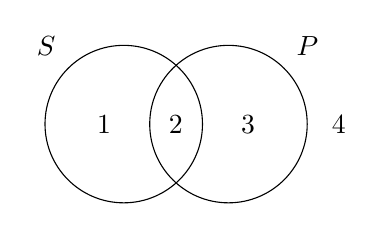
\begin{tikzpicture}
\def\firstcircle{(0,0) circle (1cm)}
\def\secondcircle{(0:1.33cm) circle (1cm)}
\draw \firstcircle node[outer sep=.75cm, above left] (s) {$S$} 
	node [xshift=-.25cm] (1) {1}
	node [xshift=.66cm] (2){2};
\draw \secondcircle node[outer sep=.75cm, above right] (p) {$P$}
	node [xshift=.25cm] (3) {3}
	node [xshift=1.4cm] (4){4};
\end{tikzpicture}
\end{center}

\noindent where area 1 represents things that are $S$ but not $P$, area 2 represents things that are both  $S$ and $P$, area 3 represents things that are only $P$, and area 4 represents things that are neither $S$ nor $P$.

Three terms give us eight possibilities to represent, so we draw the diagram like this:

\begin{center}
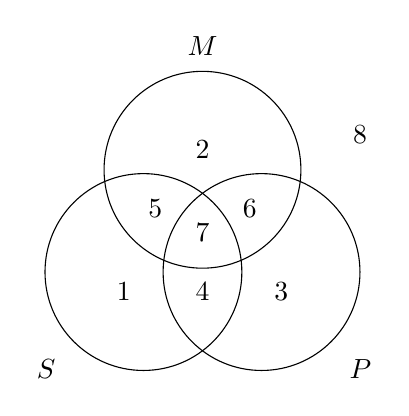
\begin{tikzpicture}
\def\firstcircle{(0,0) circle (1.25cm)}
\def\secondcircle{(60:1.5cm) circle (1.25cm)}
\def\thirdcircle{(0:1.5cm) circle (1.25cm)}

\draw \firstcircle node[outer sep=1cm, below left] {$S$}
	node [xshift=-.25cm, yshift=-.25cm](1) {1}
	node [xshift=.75cm, yshift=-.25cm] (4){4}
	node [xshift=.15cm, yshift=.8cm](5){5}
	node [xshift=.75cm, yshift=.5cm] (7){7};
\draw \secondcircle node [outer sep=1.33cm, above] {$M$}
	node [yshift=.25cm](2) {2};
\draw \thirdcircle node [outer sep=1cm, below right] {$P$}
	node [xshift=.25cm, yshift=-.25cm](3) {3}
	node[xshift=-.15cm, yshift=.8cm](6){6}
	node[xshift=1.25cm, yshift=1.75cm](8){8};  
\end{tikzpicture}
\end{center}

A four-term sorites will have 16 possible combinations of terms. To represent all of these, we will need to stretch out our circles into ellipses.   
\begin{center}
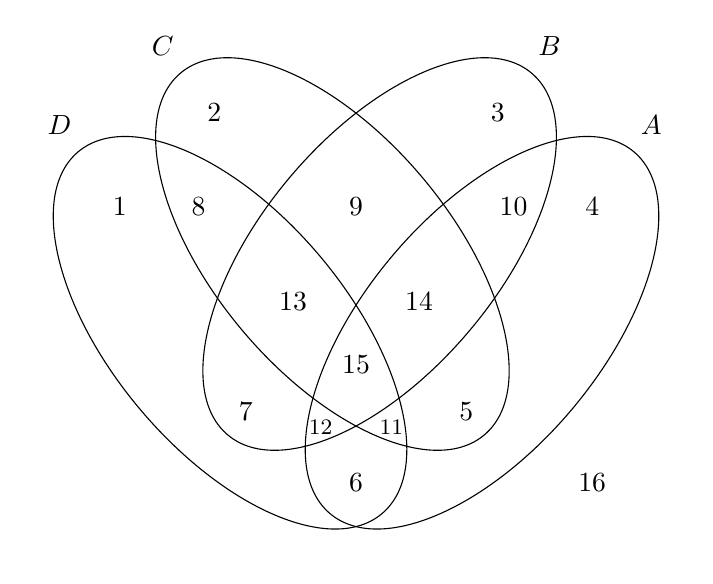
\begin{tikzpicture}
%definitions
\def\firstellip{(1.6, .4) ellipse [x radius=3cm, y radius=1.5cm,rotate=50]}
\def\secondellip{(0.3, 1.4cm) ellipse [x radius=3cm, y radius=1.5cm, rotate=50]} 
\def\thirdellip{(-0.3, 1.4cm) ellipse [x radius=3cm, y radius=1.5cm, rotate=-50]} 
\def\fourthellip{(-1.6, .4) ellipse [x radius=3cm, y radius=1.5cm, rotate=-50]} 

\draw \firstellip node [outer sep=.8cm, above right, xshift=1.1cm, yshift=1.6cm] {$A$};
\draw \secondellip node [outer sep=.8cm, above right, xshift=1.1cm, yshift=1.6cm]{$B$};
\draw \thirdellip node [outer sep=.8cm, above left, xshift=-1.1cm, yshift=1.6cm]{$C$};
\draw \fourthellip node [outer sep=.8cm, above left, xshift=-1.1cm, yshift=1.6cm] {$D$}
	node at (-3,2) {1}
	node at (-1.8,3.2) {2}
	node at (1.8,3.2) {3}
	node at (3,2) {4}
	node at (1.4,-.6) {5}
	node at (0,-1.5) {6}	
	node at (-1.4,-.6) {7}
	node at (-2,2) {8}
	node at (0,2) {9}	
	node at (2,2) {10}	
	node at (.45,-.8) {\footnotesize{11}}
	node at (-.45,-.8) {\footnotesize{12}}
	node at (-.8,.8) {13}
	node at (.8,.8) {14}
	node at (0,0) {15}
	node at (3,-1.5) {16};
\end{tikzpicture}  
\end{center}

The diagram is complex, and it takes some practice to learn to work with it. However, the basic methods for using it are the same as with the three-term diagram. Consider this argument, taken from Lewis Carroll's logic textbook \citep{Dodgson1896}.

\begin{earg}
\item[P$_1$:] Nobody who is despised can manage a crocodile.
\item[P$_2$:] Illogical persons are despised.
\item[P$_3$:] Babies are illogical.
\vspace{-.5em}
\item [] \rule{0.4\linewidth}{.5pt} 
\item[C:] No babies can manage a crocodile.
\end{earg} 

If we set the major term ``Persons who can manage a crocodile'' as $A$, the minor term ``babies'' as $D$, and the two middle terms as $B$ and $C$, we get this for the Venn diagram.

\begin{tabu}{X[1,c,m]X[1,c,m]}

\begin{ekey}
\item[$A$:] Persons who can manage a crocodile
\item[$B$:] Persons who are despised
\item[$C$:] Illogical persons
\item[$D$:] Babies
\end{ekey}

&

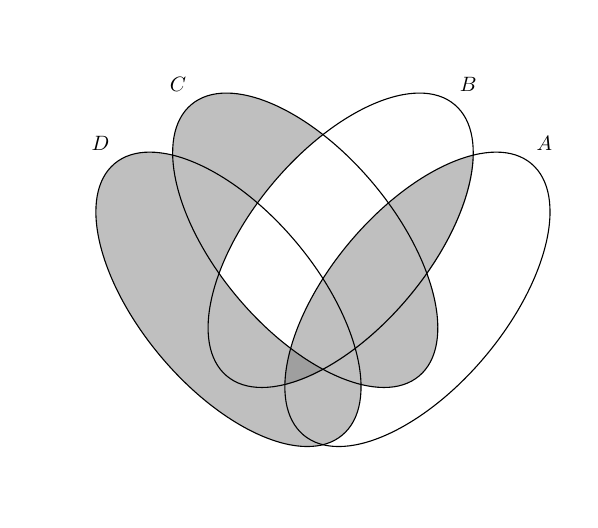
\begin{tikzpicture}[scale=.75,  every node/.style={scale=0.75}]
%definitions
\def\firstellip{(1.6, .4) ellipse [x radius=3cm, y radius=1.5cm,rotate=50]}
\def\secondellip{(0.3, 1.4cm) ellipse [x radius=3cm, y radius=1.5cm, rotate=50]} 
\def\thirdellip{(-0.3, 1.4cm) ellipse [x radius=3cm, y radius=1.5cm, rotate=-50]} 
\def\fourthellip{(-1.6, .4) ellipse [x radius=3cm, y radius=1.5cm, rotate=-50]} 

%fills
\begin{scope} %P1
\clip \firstellip; 
\filldraw[gray, opacity=.5] \secondellip;
\end{scope}

\begin{scope}[even odd rule] 
\clip \secondellip (-3,-1.55) rectangle (2,4);
\fill[gray, opacity=.5] \thirdellip;
\end{scope}

\begin{scope}[even odd rule] 
\clip \thirdellip (-5,-3) rectangle (4,5);
\fill[gray, opacity=.5] \fourthellip;
\end{scope}

%shapes

\draw \firstellip node [outer sep=.8cm, above right, xshift=1.1cm, yshift=1.6cm] {$A$};
\draw \secondellip node [outer sep=.8cm, above right, xshift=1.1cm, yshift=1.6cm]{$B$};
\draw \thirdellip node [outer sep=.8cm, above left, xshift=-1.1cm, yshift=1.6cm]{$C$};
\draw \fourthellip node [outer sep=.8cm, above left, xshift=-1.1cm, yshift=1.6cm] {$D$};
\end{tikzpicture}  

\end{tabu}

%%%%%%%%%%%%%%%%%%%%%Practice problems

\practiceproblems

\noindent\problempart \label{venn_set1} Rewrite the following arguments in standard form, reducing the number of terms if necessary. Then supply the missing intermediate conclusions and evaluate the arguments with Venn diagrams.

\begin{longtabu}{{X[1,l,p]X[9,l,p]}}
\textbf{Example}: & 
\vspace{-16pt}
\begin{earg} 
\item[P$_1$:] No $D$ are non-$B$.
\item[P$_2$:] All $B$ are $A$. 
\item[P$_3$:] No $A$ are $C$. 
\vspace{-.5em} 
\item [] \rule{0.2\linewidth}{.5pt} 
\item[C:] Some $D$ are not $C$. 
\end{earg}
\\
\textbf{Answer}: & Standard form:  \begin{earg} 
\item[P$_1$:] No $A$ are $C$.
\item[P$_2$:] All $B$ are $A$. % No $C$ are $A$
\item[P$_3$:] All $D$ are $B$.
\vspace{-.5em} 
\item [] \rule{0.2\linewidth}{.5pt} 
\item[C:] Some $D$ are not $C$. 
\end{earg}\\

&

\begin{tikzpicture}%
%%%% Venn 1
\begin{scope}
\def\firstcircle{(0,0) circle (.75cm)}
\def\secondcircle{(60:.75cm) circle (.75cm)}
\def\thirdcircle{(0:.75cm) circle (.75cm)}

\begin{scope} %shade overlap between S and M
\clip \thirdcircle;
\fill[gray] \secondcircle;
\end{scope}

\begin{scope}[even odd rule] % Shade P without M
\clip \secondcircle (-1,-1) rectangle (2,2);
\fill[gray] \firstcircle;
\end{scope}

\draw \firstcircle node[outer sep=.66cm, below left] {$B$};
\draw \secondcircle node [outer sep=.75cm, above] {$A$};
\draw \thirdcircle node [outer sep=.66cm, below right] {$C$};
\end{scope}


%%%% Venn 2
\begin{scope}[shift={(4.25cm,0cm)}]
\def\firstcircle{(0,0) circle (.75cm)}
\def\secondcircle{(60:.75cm) circle (.75cm)}
\def\thirdcircle{(0:.75cm) circle (.75cm)}

\begin{scope} %shade overlap between S and M
\clip \thirdcircle;
\fill[gray] \secondcircle;
\end{scope}

\begin{scope}[even odd rule] % Shade P without M
\clip \secondcircle (-1,-1) rectangle (2,2);
\fill[gray] \firstcircle;
\end{scope}

\draw \firstcircle node[outer sep=.66cm, below left] {$D$};
\draw \secondcircle node [outer sep=.75cm, above] {$B$};
\draw \thirdcircle node [outer sep=.66cm, below right] {$C$};
\end{scope}

%%%%%%%%%%%% Arg 1
 \node at (0,-2.65) [text width=4.5cm, outer sep=1mm] (Cesare){
\begin{earg}
\item[P$_1$:] No $A$ are $C$.
\item[P$_2$:] All $B$ are $A$. 
\vspace{-.5em}
\item [] \rule{0.7\linewidth}{.5pt} 
\item[C:] No $B$ are $C$.
\end{earg}
};

%%%%%%%%%%%% Arg 2
\node at (5.25,-2.5)[text width=4.5cm, outer sep=1mm] (Ferison){
\begin{earg}
\item[P$_1$:] No $B$ are $C$.
\item[P$_2$:] All $D$ are $B$.
\vspace{-.5em}
\item [] \rule{0.9\linewidth}{.5pt} 
\item[C:] Some $D$ are not $C$.
\end{earg}
};

\draw [myarrow1, ->] (1, -3.3) .. controls (2.125, -3.3) and (2.125, -2.15) .. (3.15, -2.15);

\node at (0,-4){\textbf{Celarent (EAE-I)}}; 	
\node at (5,-4) {\textbf{Celaront (EAO-1)}};  

\end{tikzpicture}

\\
& Conditionally valid. It also needs the premise ``Some $D$ exist.''

\end{longtabu}

\begin{exercises}

\begin{longtabu}{X[1,p,m]X[1,p,m]} 

\item \begin{earg} 
\item[P$_1$:] All $B$ are $A$.
\item[P$_2$:] Some $C$ are $D$. 
\item[P$_3$:] No $D$ are $A$.
\vspace{-.5em} 
 \item [] \rule{0.4\linewidth}{.5pt} 
\item[C:] Some $C$ are not $B$.
 \end{earg} 

%\begin{earg} 
%\item[P$_1$:] All $B$ are $A$
%\item[P$_2$:] No $D$ are $A$ %No $D$ are $B$
%\item[P$_3$:] Some $C$ are $D$
%\vspace{-.5em} 
% \item [] \rule{0.2\linewidth}{.5pt} 
%\item[C:] Some $C$ are not $B$
% \end{earg} 

% A --> B
% B --> A
% C --> D
% D --> C

&

\item \begin{earg} 
\item[P$_1$:] Some $B$ are $C$.
\item[P$_2$:] All $D$ are $A$. 
\item[P$_3$:] Some $C$ are $D$.
\vspace{-.5em} 
 \item [] \rule{0.4\linewidth}{.5pt} 
\item[C:] All $A$ are $B$.
 \end{earg}

%\begin{earg} 
%\item[P$_1$:] Some $B$ are $C$
%\item[P$_2$:] Some $C$ are $D$
%\item[P$_3$:] All $D$ are $A$
%\vspace{-.5em} 
% \item [] \rule{0.2\linewidth}{.5pt} 
%\item[C:] All $A$ are $B$
% \end{earg}

% A --> B
% B --> C
% C --> D
% D --> A

\\

\item \begin{earg} 
\item[P$_1$:] All $B$ are $C$.  
\item[P$_2$:] Some $B$ are $A$. %Some $B$ are not $D$
\item[P$_3$:] All $D$ are non-$A$. %becomes No $D$ are $A$
\vspace{-.5em} 
 \item [] \rule{0.4\linewidth}{.5pt} 
\item[C:] Some $C$ are not $D$.
 \end{earg}
 
% \begin{earg} 
%\item[P$_1$:] All $A$ are non-$B$ %becomes No $A$ are $B$
%\item[P$_2$:] Some $C$ are $B$ %Some $C$ are not $A$
%\item[P$_3$:] All $C$ are $D$ 
%\vspace{-.5em} 
% \item [] \rule{0.2\linewidth}{.5pt} 
%\item[C:] Some $D$ are not $A$.
% \end{earg}

% A --> D
% B --> A
% C --> B
% D --> C
   
%Festino (EIO-II), Bocardo (OAO-3)

&

\item \begin{earg} 
\item[P$_1$:] No $A$ are $B$.
\item[P$_2$:] No $C$ are $B$. % No $B$ are $E$
\item[P$_3$:] All $D$ are $A$.
\item[P$_4$:] All $E$ are $C$. 
\vspace{-.5em} 
 \item [] \rule{0.4\linewidth}{.5pt} 
\item[C:] No $D$ are $E$. 
 \end{earg} 

%\begin{earg} 
%\item[P$_1$:] All $E$ are $C$
%\item[P$_2$:] No $C$ are $B$ % No $B$ are $E$
%\item[P$_3$:] No $A$ are $B$
%\item[P$_4$:] All $D$ are $A$
%\vspace{-.5em} 
% \item [] \rule{0.2\linewidth}{.5pt} 
%\item[C:] No $D$ are $E$. 
% \end{earg} 

% A --> E
% B --> C
% C --> B
% D --> A
% E --> D

\\

\item \begin{earg} 
\item[P$_1$:] All $A$ are $E$.
\item[P$_2$:] All $E$ are $D$. % All $E$ are $C$  
\item[P$_3$:] All $A$ are $B$.
\item[P$_4$:] All $D$ are $C$. 
\vspace{-.5em} 
 \item [] \rule{0.4\linewidth}{.5pt} 
\item[C:] All $B$ are $C$.
 \end{earg} 

% A --> C
% B --> D
% C --> E
% D --> A
% E --> B

%\item \begin{earg} 
%\item[P$_1$:] All $D$ are $C$
%\item[P$_2$:] All $E$ are $D$ % All $E$ are $C$  
%\item[P$_3$:] All $A$ are $E$
%\item[P$_4$:] All $A$ are $B$
%\vspace{-.5em} 
% \item [] \rule{0.2\linewidth}{.5pt} 
%\item[C:] All $B$ are $C$.
% \end{earg} 

&

\item \begin{earg} 
\item[P$_1$:] All $A$ are $E$. % All $A$ are $D$  
\item[P$_2$:] All $E$ are $D$. 
\item[P$_3$:] Some $B$ are $C$.
\item[P$_4$:] All $B$ are $A$.
\vspace{-.5em} 
 \item [] \rule{0.4\linewidth}{.5pt} 
\item[C:] Some $C$ are $D$.
 \end{earg} 

%\item \begin{earg} 
%\item[P$_1$:] All $E$ are $D$
%\item[P$_2$:] All $A$ are $E$ % All $A$ are $D$  
%\item[P$_3$:] All $B$ are $A$
%\item[P$_4$:] Some $B$ are $C$
%\vspace{-.5em} 
% \item [] \rule{0.2\linewidth}{.5pt} 
%\item[C:] Some $C$ are $D$.
% \end{earg} 

% A --> D
% B --> E
% C --> A
% D --> B
% E --> C

\\

\item \begin{earg} 
\item[P$_1$:] All $A$ are $B$.
\item[P$_2$:] No $C$ are $E$. 
\item[P$_3$:] No $D$ are non-$A$.	%Some $A$ are not $C$
\item[P$_4$:] Some $E$ are $D$. %Some $D$ are not $C$
\vspace{-.5em} 
 \item [] \rule{0.4\linewidth}{.5pt} 
\item[C:] Some $B$ are not $C$.
 \end{earg} 

%\begin{earg} 
%\item[P$_1$:] No $C$ are $E$
%\item[P$_2$:] Some $E$ are $D$ %Some $D$ are not $C$
%\item[P$_3$:] No $D$ are non-$A$	%Some $A$ are not $C$
%\item[P$_4$:] All $A$ are $B$
%\vspace{-.5em} 
% \item [] \rule{0.6\linewidth}{.5pt} 
%\item[C:] Some $B$ are not $C$
% \end{earg} 

% A --> C
% B --> E
% C --> D
% D --> A
% E --> B

&

\item \begin{earg} 
\item[P$_1$:] All $D$ are $A$. % Some $A$ are not $E$
\item[P$_2$:] All $A$ are $C$.
\item[P$_3$:] All $E$ are $B$. 
\item[P$_4$:] Some $D$ are not $B$. %  Some $D$ are not $E$
\vspace{-.5em} 
 \item [] \rule{0.4\linewidth}{.5pt} 
\item[C:] Some $C$ are not $E$.
 \end{earg} 

%\begin{earg} 
%\item[P$_1$:] All $E$ are $B$
%\item[P$_2$:] Some $D$ are not $B$ %  Some $D$ are not $E$
%\item[P$_3$:] All $D$ are $A$ % Some $A$ are not $E$
%\item[P$_4$:] All $A$ are $C$
%\vspace{-.5em} 
% \item [] \rule{0.2\linewidth}{.5pt} 
%\item[C:] Some $C$ are not $E$
% \end{earg} 

% A --> E
% B --> B
% C --> D
% D --> A
% E --> C

\\

\item \begin{earg} 
\item[P$_1$:] All $E$ are $D$. %  Some $D$ are not $F$ 
\item[P$_2$:] No $E$ are $F$.
\item[P$_3$:] All $B$ are $A$. 
\item[P$_4$:] All $C$ are $B$.  
\item[P$_5$:] All $D$ are $C$.  
\vspace{-.5em} 
 \item [] \rule{0.4\linewidth}{.5pt} 
\item[C:] Some $A$ are not $F$.
 \end{earg} 

 % A --> F
% B --> E
% C --> D
% D --> C
% E --> B
% F --> A
% 5 term conditionally valid.  
&

\item \begin{earg} 
\item[P$_1$:] All $B$ are $A$. 
\item[P$_2$:] Some $C$ are $E$. %  Some $C$ are $F$
\item[P$_3$:] No $A$ are $D$.
\item[P$_4$:] All $C$ are $B$.%   %
\item[P$_5$:] All $E$ are $F$. 
\vspace{-.5em} 
\item [] \rule{0.4\linewidth}{.5pt} 
\item[C:] Some $D$ are $F$.
 \end{earg} 
%5 premises term reduction invalid 2
% A --> F
% B --> E
% C --> C
% D -->B
% E --> A
% F --> D 

\end{longtabu}

\end{exercises}

\noindent\problempart \label{venn_set2} Rewrite the following arguments in standard form, reducing the number of terms if necessary. Then supply the missing intermediate conclusions and evaluate the arguments with Venn diagrams.

\begin{exercises}
\begin{longtabu}{X[1,p,m]X[1,p,m]} 
\item \begin{earg}
\item[P$_1$:] No $D$ are $C$.
\item[P$_2$:] No $A$ are $B$. 
\item[P$_3$:] Some $D$ are $A$ %Some $D$ are not $B$
\vspace{-.5em}
\item [] \rule{0.4\linewidth}{.5pt} 
\item[C:] Some $C$ are not $B$.
\end{earg} 
%3 premise, invalid

% * P --> B
% * M --> A
% * M2 --> D
% * S --> C

& 
\item \begin{earg}
\item[P$_1$:] All $C$ are $B$.
\item[P$_2$:] No $B$ are $D$. %  No $D$ are $C$
\item[P$_3$:] All $A$ are $D$.
\vspace{-.5em}
\item [] \rule{0.4\linewidth}{.5pt} 
\item[C:] Some $A$ are not $C$.
\end{earg} 
%3 premise, conditionally valid--EA family

% * P -->  C
% * M --> B
% * M2 --> D
% * S --> A

\\
\item \begin{earg}
\item[P$_1$:] Some $M$ are not $P$.
\item[P$_2$:] No $M$ are non-$M2$. % Some M2 are not $P$
\item[P$_3$:] No $M2$ are non-$S$.
\vspace{-.5em}
\item [] \rule{0.4\linewidth}{.5pt} 
\item[C:] Some $S$ are not $P$.
\end{earg} 
%3 premise, reduce terms

% * P --> D
% * M --> C
% * M2 --> B
% * S --> A

&
\item \begin{earg}
\item[P$_1$:] All $A$ are $B$. %some $A$ are $C$
\item[P$_2$:] All $E$ are $A$.
\item[P$_3$:] All $D$ are $C$.
\item[P$_4$:] All $D$ are $B$. % Some $B$ are $C$
\vspace{-.5em}
\item [] \rule{0.4\linewidth}{.5pt} 
\item[C:] Some $E$ are $C$.
\end{earg} 
%4 premise, conditionally valid--AI family

% * P --> C
% * M --> D
% * M2 --> B
% * M3 --> A
% * S --> E 
\\
\item \begin{earg}
\item[P$_1$:] Some $E$ are $C$. % Some $C$ are $D$
\item[P$_2$:] Some $A$ are $C$.
\item[P$_3$:] All $B$ are $D$.
\item[P$_4$:] All $E$ are $B$.	%All $E$ are $D$
\vspace{-.5em}
\item [] \rule{0.4\linewidth}{.5pt} 
\item[C:] Some $A$ are $D$. 
\end{earg} 
%4 premise

% * P --> D
% * M --> B
% * M2 --> E
% * M3 --> C
% * S --> A

&
\item \begin{earg}
\item[P$_1$:] No $B$ are $C$.
\item[P$_2$:] Some $B$ are not $A$. % Some $B$ are not $E$ 
\item[P$_3$:] All $C$ are $D$.
\item[P$_4$:] All $E$ are $A$.
\vspace{-.5em}
\item [] \rule{0.4\linewidth}{.5pt} 
\item[C:] Some $D$ are not $E$. 
\end{earg} 
%4 premise, invalid

% * P --> E
% * M --> A
% * M2 --> B
% * M3 --> C
% * S --> D

\\
\item \begin{earg}
\item[P$_1$:] All $D$ are $A$.
\item[P$_2$:] All $C$ are $D$.
\item[P$_3$:] No $E$ are $B$.
\item[P$_4$:] No $B$ are $A$.
\vspace{-.5em}
\item [] \rule{0.4\linewidth}{.5pt} 
\item[C:] No $C$ are $E$. 
\end{earg} 
%4 premise, invalid

% * P --> E
% * M --> B
% * M2 --> A
% * M3 --> D
% * S --> C

&
\item \begin{earg}
\item[P$_1$:] No $A$ are non-$D$.
\item[P$_2$:] No $D$ are $C$. %No $C$ are $A$
\item[P$_3$:] All $B$ are $C$. %No $B$ are $A$
\item[P$_4$:] All non-$B$ are non-$E$
\vspace{-.5em}
\item [] \rule{0.4\linewidth}{.5pt} 
\item[C:] No $E$ are $A$.
\end{earg} 
%4 premise, reduce terms

% * P --> A
% * M --> D
% * M2 --> C
% * M3 --> B
% * S --> E

\\
\item \begin{earg}
\item[P$_1$:] No $E$ are $F$.
\item[P$_2$:] All $D$ are $B$. % All $D$ are $A$
\item[P$_3$:] All $C$ are $E$.
\item[P$_4$:] Some $D$ are not $F$.
\item[P$_5$:] All $B$ are $A$.
\vspace{-.5em}
\item [] \rule{0.4\linewidth}{.5pt} 
\item[C:] Some $C$ are not $A$.
\end{earg} 
%5 premise, invalid

% * P --> A
% * M --> B
% * M2 --> D
% * M3 --> F
% * M4 --> E
% * S --> C

&
\item \begin{earg}
\item[P$_1$:] No $B$ are $D$.
\item[P$_2$:] All $E$ are $A$.
\item[P$_3$:] All $F$ are $C$. %All $F$ are $A$
\item[P$_4$:] All $C$ are $E$. % All $C$ are $A$
\item[P$_5$:] All $D$ are $F$. % All $D$ are $A$
\vspace{-.5em}
\item [] \rule{0.4\linewidth}{.5pt} 
\item[C:] No $B$ are $A$. 
\end{earg} 
%5 premise, reduce terms

% * P --> A
% * M --> E
% * M2 --> C
% * M3 --> F
% * M4 --> D
% * S --> B

\end{longtabu}
\end{exercises}

\noindent\problempart Do the exercises in Part \ref{venn_set1}, but skip writing out the missing intermediate conclusions, and evaluate them using the rules method instead of the Venn diagram method.

\begin{longtabu}{p{.1\linewidth}p{.9\linewidth}}

\textbf{Example}: & \vspace{-16pt} \begin{earg} 
\item[P$_1$:] No $D$ are non-$B$.
\item[P$_2$:] All $B$ are $A$. 
\item[P$_3$:] No $A$ are $C$. 
\vspace{-.5em} 
\item [] \rule{0.3\linewidth}{.5pt} 
\item[C:] Some $D$ are not $C$. 
\end{earg} \\
\textbf{Answer}: & \vspace{-16pt} \begin{earg} 
\item[P$_1$:] No $A$\textsuperscript{D} are $C$\textsuperscript{D}.
\item[P$_2$:] All $B$\textsuperscript{D} are $A$. % No $C$ are $A$
\item[P$_3$:] All $D$\textsuperscript{D} are $B$.
\vspace{-.5em} 
\item [] \rule{0.3\linewidth}{.5pt} 
\item[C:] Some $D$ are not $C$\textsuperscript{D}. 
\end{earg}
\\ & 
\textbf{Rule 1:} Pass. Middle terms $A$ and $B$ are distributed in P$_1$ and P$_2$. \newline
\textbf{Rule 2:} Pass. The conclusion distributes $C$, which is also distributed in  P$_1$.\newline
\textbf{Rule 3:} Pass. There is one negative premise, P$_1$. \newline
\textbf{Rule 4:} Pass. The conclusion is negative, and there is exactly one negative premise.\newline
\textbf{Rule 5:} Fail. The premises are all universal and the conclusion is particular. \\
& Conditionally valid. It needs the premise ``Some $D$ exist.''
\end{longtabu}


\noindent\problempart Do the exercises in Part \ref{venn_set2}, but skip writing out the missing intermediate conclusions, and evaluate them using the rules method instead of the Venn diagram method.


\noindent\problempart  Rewrite the following arguments in standard form, reducing terms if necessary, and then prove that they are valid using a single, four-term Venn diagram.

\begin{longtabu}{p{.1\linewidth}p{.8\linewidth}}

\textbf{Example}: & \vspace{-16pt} \begin{earg} 
\item[P$_1$:] No $D$ are non-$B$.
\item[P$_2$:] All $B$ are $A$. 
\item[P$_3$:] No $A$ are $C$. 
\vspace{-.5em} 
\item [] \rule{0.3\linewidth}{.5pt} 
\item[C:] Some $D$ are not $C$. 
\end{earg} \\
\textbf{Answer}: & \vspace{-16pt} \begin{earg} 
\item[P$_1$:] No $A$ are $C$.
\item[P$_2$:] All $B$ are $A$. % No $C$ are $A$
\item[P$_3$:] All $D$ are $B$.
\vspace{-.5em} 
\item [] \rule{0.3\linewidth}{.5pt} 
\item[C:] Some $D$ are not $C$.
\end{earg}
\\ & 

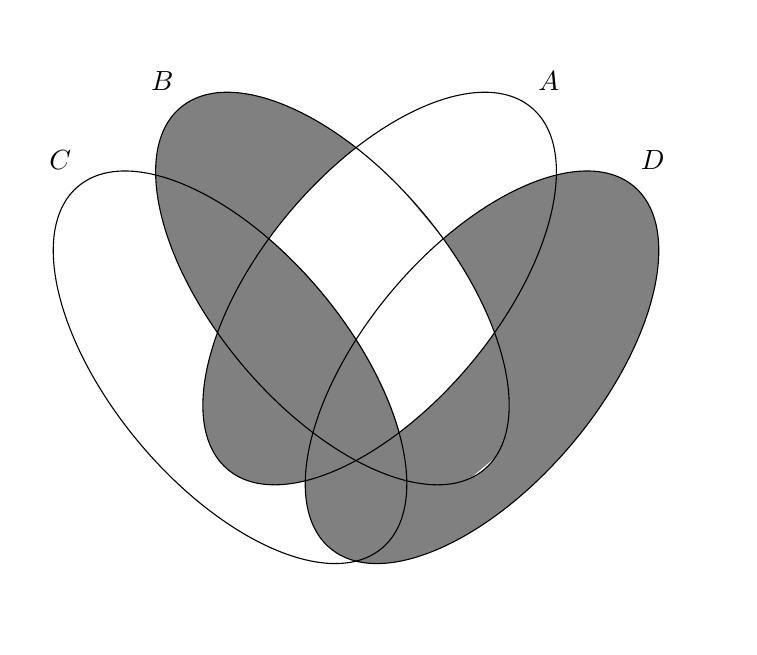
\begin{tikzpicture}

%definitions
\def\firstellip{(1.6, .4) ellipse [x radius=3cm, y radius=1.5cm,rotate=50]}
%
\def\secondellip{(0.3, 1.4cm) ellipse [x radius=3cm, y radius=1.5cm, rotate=50]} 

\def\thirdellip{(-0.3, 1.4cm) ellipse [x radius=3cm, y radius=1.5cm, rotate=-50]} 

\def\fourthellip{(-1.6, .4) ellipse [x radius=3cm, y radius=1.5cm, rotate=-50]} 

\def\firstrect{[rotate around={50:(.85, -2.9)}](.85, -2.9) rectangle ++(6.05, 3.05)}

\def\secondrect{[rotate around={50:(-.45, -1.85)}](-.45, -1.85) rectangle ++(6.05, 3)}

\def\thirdrect{[rotate around={-50:(.45, -1.85)}](.45, -1.85) rectangle ++(-6.05, 3)}

\def\fourthrect{[rotate around={-50:(-.85, -2.9)}](-.85, -2.9) rectangle ++(-6.05, 3.05)}

\def\bounding{(-5,-3) rectangle (5,4)}

%fills

\begin{scope} %P1
\clip \secondellip; 
\filldraw[gray] \fourthellip;
\end{scope}
%
\begin{scope}[even odd rule] 
\clip \secondellip \thirdrect;
\fill[gray] \thirdellip;
\end{scope}

\begin{scope}[even odd rule] 
\clip \thirdellip \firstrect;
\fill[gray] \firstellip;
\end{scope}

%shapes

\draw \firstellip node [outer sep=.8cm, above right, xshift=1.1cm, yshift=1.6cm] {$D$};

\draw \secondellip node [outer sep=.8cm, above right, xshift=1.1cm, yshift=1.6cm]{$A$};

\draw \thirdellip node [outer sep=.8cm, above left, xshift=-1.1cm, yshift=1.6cm]{$B$};

\draw \fourthellip node [outer sep=.8cm, above left, xshift=-1.1cm, yshift=1.6cm] {$C$};
\end{tikzpicture}  

Conditionally valid. If you had a premise that told you to write an x in the $D$ ellipse, it would clearly fall outside of $C$.

\end{longtabu}


\begin{exercises}
\begin{longtabu}{X[1,p,m]X[1,p,m]} 
\item \begin{earg}
\item[P$_1$:] No $D$ are $B$. 
\item[P$_2$:] All $A$ are $C$.
\item[P$_3$:] All $C$ are $B$.
\vspace{-.5em}
\item [] \rule{0.6\linewidth}{.5pt} 
\item[C:] No $D$ are $A$.
\end{earg} 

% Invalid
% * P --> A
% * M1 --> C 
% * M2 --> B
% * S --> D

&
\item\begin{earg}
\item[P$_1$:] All $A$ are $B$.
\item[P$_2$:] No $D$ are $C$.
\item[P$_3$:] All $C$ are $A$. % All C are B
\vspace{-.5em}
\item [] \rule{0.3\linewidth}{.5pt} 
\item[C:] No $D$ are $B$.
\end{earg}

% Valid
% * P --> B
% * M1 --> A
% * M2 --> C
% * S --> D

\\
\item\begin{earg}
\item[P$_1$:] All $B$ are $D$. %Some $B$ are not $A$
\item[P$_2$:] All $B$ are $C$.
\item[P$_3$:] No $A$ are $D$.
\vspace{-.5em}
\item [] \rule{0.3\linewidth}{.5pt} 
\item[C:] Some $C$ are not $A$.
\end{earg}

% conditionally valid
% * P --> A
% * M1 --> D
% * M2 --> B
% * S --> C

&
\item\begin{earg}
\item[P$_1$:] No $A$ are $C$.
\item[P$_2$:] All $B$ are $D$.
\item[P$_3$:] All $C$ are $B$. %All C are D
\vspace{-.5em}
\item [] \rule{0.6\linewidth}{.5pt} 
\item[C:] No $A$ are $D$.
\end{earg}

% Valid, reduce terms
% * P --> D
% * M1 --> B
% * M2 --> C
% * S --> A

\\
\item\begin{earg}
\item[P$_1$:] All $D$ are $A$.
\item[P$_2$:] Some $C$ are $B$.
\item[P$_3$:] Some $B$ are not $D$.
\vspace{-.5em}
\item [] \rule{0.6\linewidth}{.5pt} 
\item[C:] Some non-$C$ are not non-$A$.
\end{earg}

% Invalid, reduce terms
% * P --> C
% * M1 --> B 
% * M2 --> D
% * S --> A

&
\end{longtabu}
\end{exercises}

\noindent\problempart  Rewrite the following arguments in standard form, reducing terms if necessary, and then prove that they are valid using a single, four-term Venn diagram.
            
\begin{exercises}
\begin{longtabu}{X[1,p,m]X[1,p,m]} 
\item \begin{earg}
\item[P$_1$:] No $A$ are $C$.
\item[P$_2$:] All $B$ are $D$.
\item[P$_3$:] Some $B$ are $A$.
\vspace{-.5em}
\item [] \rule{0.6\linewidth}{.5pt} 
\item[C:] Some $S$ are not $C$.
\end{earg} 
%
%% Valid
%% * P --> C
%% * M1 --> A
%% * M2 --> B
%% * S --> D
%
&
\item\begin{earg}
\item[P$_1$:] No $P$ are $M$.
\item[P$_2$:] All $M$ are $M2$.
\item[P$_3$:] No $M2$ are $S$.
\vspace{-.5em}
\item [] \rule{0.6\linewidth}{.5pt} 
\item[C:] No $S$ are $P$.
\end{earg}
%
%% Invalid
%% * P --> B
%% * M1 --> A
%% * M2 --> C
%% * S --> D
%
\\
\item\begin{earg}
\item[P$_1$:] All $A$ are $C$.
\item[P$_2$:] All $B$ are $C$.
\item[P$_3$:] All $A$ are $D$.
\vspace{-.5em}
\item [] \rule{0.6\linewidth}{.5pt} 
\item[C:] Some $D$ are $B$.
\end{earg}

% Conditionally  valid
% * P --> B
% * M1 --> C
% * M2 --> A
% * S --> D

&
\item\begin{earg}
\item[P$_1$:] Some non-$D$ are not non-$C$.
\item[P$_2$:] All $D$ are $B$.
\item[P$_3$:] No $B$ are $A$.
\vspace{-.5em}
\item [] \rule{0.6\linewidth}{.5pt} 
\item[C:] Some $A$ are not $C$.
\end{earg}
% Invalid, reduce terms
% * P --> C
% * M1 --> D
% * M2 --> B
% * S --> A
\\
\item\begin{earg}
\item[P$_1$:] No $C$ are non-$B$.
\item[P$_2$:] Some $D$ are $A$.
\item[P$_3$:] All $D$ are $C$. %Some $C$ are $A$
\vspace{-.5em}
\item [] \rule{0.6\linewidth}{.5pt} 
\item[C:] Some $B$ are not $A$.
\end{earg}
% Valid, reduce terms
% * P --> A
% * M1 --> D
% * M2 --> C
% * S --> B

\end{longtabu}
\end{exercises}

\noindent\problempart Rewrite the following arguments in standard form using variables and a translation key. Then evaluate using any method you want. The example problem, along with exercises \ref{itm:sons}, \ref{itm:ducks},  \ref{itm:Auk}, and \ref{itm:rainbow}, come from Lewis Carroll's logic textbook \citep{Dodgson1896}. Other exercises are just Lewis Carroll themed.

\begin{longtabu}{p{.1\linewidth}p{.5\linewidth}p{.4\linewidth}}

\textbf{Example}: & \multicolumn{2}{p{.9\linewidth}}{My saucepans are the only things I have that are made of tin. I find all your presents very useful, but none of my saucepans are of the slightest use. Therefore, none of your presents are made of tin.} \\
\\
\textbf{Answer}:&
\vspace{-.5cm}
\begin{ekey}
\item[$A$:]Things of mine made from tin
\item[$B$:] Saucepans
\item[$C$:] Useful things 
\item[$D$:] Presents from you
\end{ekey}

& 
\vspace{-.5cm}
\begin{earg}
\item[P$_1$:] All $A$ are $B$.
\item[P$_2$:] No $B$ are $C$.
\item[P$_3$:] All $D$ are $C$. 
\vspace{-.5em}
\item [] \rule{0.6\linewidth}{.5pt} 
\item[C:] No $D$ are $A$.
\end{earg}
\end{longtabu}
\vspace{-.75cm}
\begin{center}
\begin{tikzpicture}
\begin{scope}
% venns
\begin{scope}
\def\firstcircle{(0,0) circle (.75cm)}
\def\secondcircle{(60:.75cm) circle (.75cm)}
\def\thirdcircle{(0:.75cm) circle (.75cm)}

\begin{scope} 
\clip \thirdcircle;
\fill[gray] \secondcircle;
\end{scope}

\begin{scope}[even odd rule] % Shade P without M
\clip \secondcircle (-1,-1) rectangle (2,2);
\fill[gray] \firstcircle;
\end{scope}

\draw \firstcircle node[outer sep=.66cm, below left] {$A$};
\draw \secondcircle node [outer sep=.75cm, above] {$B$};
\draw \thirdcircle node [outer sep=.66cm, below right] {$C$};

\end{scope}

\begin{scope}[xshift=4cm]

\def\firstcircle{(0,0) circle (.75cm)}
\def\secondcircle{(60:.75cm) circle (.75cm)}
\def\thirdcircle{(0:.75cm) circle (.75cm)}

\begin{scope} %shade overlap between S and M
\clip \thirdcircle;
\fill[gray] \secondcircle;
\end{scope}

\begin{scope}[even odd rule] % Shade P without M
\clip \secondcircle (-1,-1) rectangle (2,2);
\fill[gray] \firstcircle;
\end{scope}

\draw \secondcircle node [outer sep=.75cm, above] {$C$};
\draw \thirdcircle node [outer sep=.66cm, below right] {$A$};
\draw \firstcircle node[outer sep=.66cm, below left] {$D$};

\end{scope}

%% args

\node at (0,-2.5)[text width=4.5cm, outer sep=1mm] (Celarent){ 
\begin{earg}
\item[P$_1$:] All $A$ are $B$.
\item[P$_2$:] No $B$ are $C$.
\vspace{-.5em}
\item [] \rule{0.6\linewidth}{.5pt} 
\item[C:] No $A$ are $C$.* 
\end{earg} 

};

\node at (-.1, -3.9) {\textbf{Celarent (EAE-I)}};

\draw [myarrow1, ->] (1.1, -3.05) .. controls (2.4, -3) and (2.4, -2) .. (3.3, -1.95);
%
%\filldraw [red] (0,0) circle (.1cm);
%\filldraw [red] (2.4, -.5) circle (.1cm); 
%\filldraw [red] (2.4, .5)  circle (.1cm);

\node at (5,-2.3)[text width=4.5cm, outer sep=1mm] { 
\begin{earg} 
\item[P$_1$:] No $A$ are $C$.*
\item[P$_2$:] All $D$ are $C$.
\vspace{-.5em} 
\item [] \rule{0.6\linewidth}{.5pt} 
\item[C:] No $D$ are $A$.
\end{earg}
%Cesare (EAE-II)
};

\node at (4.9, -3.9) {\textbf{Cesare (EAE-II)}};
\end{scope}
\end{tikzpicture}
\end{center}

\begin{exercises}

\item All metal things are solid, and some of those metal things are also chairs. All chairs are furniture. Therefore some solid things are furniture. 

%Three premise valid


%\begin{earg} 
%\item[P$_1$:] All $M1$ are $P$
%\item[P$_2$:] Some $M2$ are $M1$
%\item[P$_3$:] All $M2$ are $S$
%\vspace{-.5em} 
% \item [] \rule{0.6\linewidth}{.5pt} 
%\item[C:] Some $S$ are $P$
% \end{earg}


\item \label{itm:sons} Every one who is sane can do Logic. No lunatics are fit to serve on a jury. None of \textit{your} sons can do Logic. Therefore, none of your sons can serve on a jury.

%three premise valid

\item All hat-wearers are heaven-sent. This is because all platypuses are heaven-sent, all secret agents are platypuses, and some secret agents wear hats. 

%\begin{earg} 
%\item[P$_1$:] All platypuses are heaven-sent
%\item[P$_2$:] All secret agents are platypuses     %All $C$ are $A$
%\item[P$_3$:] Some secret agents wear hats
%\vspace{-.5em} 
% \item [] \rule{0.6\linewidth}{.5pt} 
%\item[C:] All hat-wearers are heaven-sent
% \end{earg}


\item \label{itm:ducks} No ducks waltz. No officers ever decline to waltz. All my poultry are ducks. Therefore, none of my poultry are officers.



%\begin{earg}
%\item[P$_1$:] All my poultry are ducks
%\item[P$_2$:] No ducks waltz 
%\item[P$_3$:] All officers waltz 
%\vspace{-.5em}
%\item [] \rule{0.6\linewidth}{.5pt} 
%\item[C:] None of my poultry are officers
%\end{earg} 

\item Some things are uffish, but nothing that is uffish is vorpal. Therefore some uffish things are not swords, because everything that is vorpal goes snicker-snack, and everything that goes snicker-snack is a sword. 

%\begin{ekey}
%\item[$A$:] Swords. 
%\item[$B$:] Things that go snicker-snack
%\item[$C$:] Vorpal things.
%\item[$D$:] Uffish things
%\end{ekey}



%\begin{earg}
%\item[P$_1$:] Everything that goes snicker-snack is a sword.
%\item[P$_2$:] Everything that is vorpal goes snicker-snack  
%& Everything that is vorpal is a sword
%\item[P$_3$:] Nothing uffish is vorpal
%\item[{\color{red}P$_4$:}] {\color{red}Some uffish things exist.}
%\vspace{-.5em}
%\item [] \rule{0.2\linewidth}{.5pt} 
%\item[C:] Some uffish things are not swords
%\end{earg} 

%\begin{earg}
%\item[P$_1$:] All $B$ are $A$.
%\item[P$_2$:] All $C$ are $B$
%\item[P$_3$:] No $D$ are $C$
%\item[{\color{red}P$_4$:}] {\color{red}$D$ exists.}
%\vspace{-.5em}
%\item [] \rule{0.2\linewidth}{.5pt} 
%\item[C:] Some $D$ are not $A$
%\end{earg} 

\item No animals are plants. Some animals are mammals. Some mammals are dogs. All dachshunds are dogs. Therefore, no dachshunds are plants.


%\begin{earg}
%\item[P$_1$:] No $B$ are $A$
%\item[P$_2$:] Some $B$ are $C$.    % Therefore, some $C$ are not $A$. 
%\item[P$_3$:] Some $C$ are $D$     
%\item[P$_4$:] All $E$ are $D$
%\vspace{-.5em}
%\item [] \rule{0.6\linewidth}{.5pt} 
%\item[C:]  No $E$ are $A$. 
%\end{earg} 


\item \label{itm:Auk} Things sold in the street are of no great value. Nothing but rubbish can be had for a song. Eggs of the Great Auk are very valuable. It is only what is sold in the streets that is really rubbish. Therefore the eggs of the Great Auk cannot be had for a song.

%\begin{earg}
%\item[P$_1$:] Nothing but rubbish can be had for a song
%\item[P$_2$:] It is only what is sold in the streets that is really rubbish.
%\item[P$_3$:] Things sold in the street are of no great value; 
%\item[P$_3$:] Eggs of the Great Auk are very valuable
%\vspace{-.5em}
%\item [] \rule{0.6\linewidth}{.5pt} 
%\item[C:] The eggs of the Great Auk cannot be had for a song
%\end{earg} 

%\begin{ekey}
%\item[$A$:] Things you can have for a song
%\item[$B$:] Rubbish
%\item[$C$:] Valuable things
%\item[$D$:] Things sold in the street
%\item[$E$:] Eggs of the Great Auk
%\end{ekey}

%\begin{earg}
%\item[P$_1$:] All $A$ are $B$
%\item[P$_2$:] All $B$ are $C$
%\item[P$_3$:] No $C$ are $D$; 
%\item[P$_3$:] All $E$ are $D$
%\vspace{-.5em}
%\item [] \rule{0.6\linewidth}{.5pt} 
%\item[C:] No E are A.
%\end{earg} 

\item All life forms are physical objects, and all bacteria are life forms. Also, all \textit{E. coli} are bacteria, so all rod shaped things are physical objects, because all \textit{E. coli} are rod-shaped. 
   
% four premise invalid 
 
%\begin{earg}
%\item[P$_1$:] All $B$ are $A$
%\item[P$_2$:] All $C$ are $B$
%\item[P$_3$:] All $D$ are $C$; 
%\item[P$_4$:] All $D$ are $E$
%\vspace{-.5em}
%\item [] \rule{0.6\linewidth}{.5pt} 
%\item[C:] All E are A.
%\end{earg}  




\item Some playing cards shout ``Off with his head!'' All playing cards play croquet. Everyone who plays croquet uses hedgehogs for balls. Everyone who uses hedgehogs for balls uses flamingos for mallets. The queen of hearts uses flamingos for mallets. Therefore some cards identical to the queen of hearts shout ``Off with his head!''

%Playing cards
%``shout off with his head'!'
%Plays croquet 
%Uses hedgehogs for balls 
%uses flamingos for mallets
%Is identical to the queen of hearts

%\begin{earg} 
%\item[P$_1$:] Some $B$ are $A$
%\item[P$_2$:] All $B$ are $C$     %Some $C$ are $A$ 	Disamis (IAI-III) (valid) 
% \item[P$_3$:] All $C$ are $D$ 	% Some $D$ are $A$ %		Disamis (IAI-III) (valid) 
%\item[P$_4$:] All $D$ are $E$ % Some $E$ are $A$ Disamis (IAI-III) (valid) 
%\item[P$_5$:] All $F$ are $E$ 
% \item [] \rule{0.6\linewidth}{.5pt} 
%\item[C:] Some $F$ are $A$ % IAI-I (invalid) 
% \end{earg} 

%\begin{earg} 
%\item[P$_1$:] Some $B$ are $A$
%\item[P$_2$:] All $B$ are $C$
%\vspace{-.5em} 
% \item [] \rule{0.6\linewidth}{.5pt} 
%\item[IC$_1$:] Some $C$ are $A$
% \end{earg} Disamis (IAI-III) (valid) 

%\begin{earg} 
%\item[IC$_1$:] Some $C$ are $A$
%\item[P$_3$:] All $C$ are $D$
%\vspace{-.5em} 
% \item [] \rule{0.6\linewidth}{.5pt} 
%\item[IC$_2$:] Some $D$ are $A$
% \end{earg} Disamis (IAI-III) (valid) 

%\begin{earg} 
%\item[IC$_2$:] Some $D$ are $A$
%\item[P$_4$:] All $D$ are $E$
%\vspace{-.5em} 
% \item [] \rule{0.6\linewidth}{.5pt} 
%\item[IC$_3$:] Some $E$ are $A$
% \end{earg} Disamis (IAI-III) (valid) 

%\begin{earg} 
%\item[IC$_3$:] Some $E$ are $A$
%\item[P$_5$:] All $F$ are $E$ 
% \item [] \rule{0.6\linewidth}{.5pt} 
%\item[C:] Some $F$ are $A$
% \end{earg} IAI-I (invalid) 



\item \label{itm:rainbow} I despise anything that cannot be used as a bridge. Everything, that is worth writing an ode to, would be a welcome gift to me. A rainbow will not bear the weight of a wheelbarrow.  Whatever can be used as a bridge will bear the weight of a wheel-barrow. I would not take, as a gift, a thing that I despise. Therefore a rainbow is not worth writing an ode to. 

%\begin{earg}
%\item[P$_1$:] Everything, that is worth writing an ode to, would be a welcome gift to me
%\item[P$_2$:] I would not take, as a gift, a thing that I despise. 
%\item[P$_3$:] I despise anything that cannot be used as a bridge;
%\item[P$_4$:] Whatever can be used as a bridge will bear the weight of a wheel-barrow; 
%\item[P$_5$:] A rainbow will not bear the weight of a wheelbarrow; 
%\vspace{-.5em}
%\item [] \rule{0.6\linewidth}{.5pt} 
%\item[C:] A rainbow is not worth writing an ode to. 
%\end{earg} 
\end{exercises}

\noindent\problempart Rewrite the following arguments in standard form using variables and a translation key, and supply intermediate conclusions. Then evaluate using any method you want. Exercises \ref{itm:talkers}, \ref{itm:hedgehogs}, \ref{itm:mermaids}, \ref{itm:books}, and \ref{itm: poems} come from Lewis Carroll's logic textbook \citep{Dodgson1896}. Other exercises are just Lewis Carroll themed.

\begin{exercises}

\item All buildings are habitable places, and all houses are residences. Therefore all houses are buildings because all residences are habitable places. 

%\begin{earg}
%\item[P$_1$:] All $A$ are $B$
%\item[P$_2$:] All $C$ are $B$		%All $C$ are $A$
%\item[P$_3$:] All $D$ are $C$
%\vspace{-.5em}
%\item [] \rule{0.6\linewidth}{.5pt} 
%\item[C:]  All $D$ are $A$
%\end{earg} 


\item Not all cephalopods are moralizing, but cuttlefish are. All pompous squid are cephalopods. Therefore some pompous squid are not cuttlefish. 

%
%\begin{earg}
%\item[P$_1$:] All $A$ are $B$
%\item[P$_2$:] Some $C$ are not $B$		%Some $C$ are not $A$
%\item[P$_3$:] All $D$ are $C$
%\vspace{-.5em}
%\item [] \rule{0.6\linewidth}{.5pt} 
%\item[C:] Some $D$ are not $A$
%\end{earg} 

%AEE-II, EAO-1


\item \label{itm:talkers} Showy talkers think too much of themselves; No really well-informed people are bad company; and people who think too much of themselves are not good company. Therefore no showy talkers are really well informed. %[three premise] LC 


%\begin{earg}
%\item[P$_1$:] No really well-informed people are bad company; 
%\item[P$_2$:] People who think too much of themselves are not good company.
%\item[P$_3$:] Showy talkers think too much of themselves; 
%\vspace{-.5em}
%\item [] \rule{0.6\linewidth}{.5pt} 
%\item[C:] No one who thinks too much of themselves is really well informed.
%\end{earg} 

%\begin{ekey}
%\item[$A$:] Well informed people.
%\item[$B$:] Good company
%\item[$C$:] People who think too much of themselves.
%\item[$D$:] Showy talkers
%\end{ekey}

%\begin{earg}
%\item[P$_1$:] All $A$ are $B$    %No $A$ are non-$B$
%\item[P$_2$:] No $C$ are $B$.    %No $C$ are $A$ camestres
%\item[P$_3$:] All $C$ are $D$; 
%\vspace{-.5em}
%\item [] \rule{0.6\linewidth}{.5pt} 
%\item[C:] No $D$ are $A$
%\end{earg} 



\item All white animals are late, and some late animals are rabbits. Also, all animals taking a watch out of their waistcoat pocket are white. Therefore, some rabbits are taking a watch out of their waistcoat pocket.


%$A$: animals taking a watch out of their waistcoat pocket. 
%B: White animals
%C: Late animals
%D: Rabbits


%\begin{earg}
%\item[P$_1$:] All animals taking a watch out of their waist-coat pocket are white
%\item[P$_2$:] All white animals are late 			All $M2$ are $P$
%\item[P$_3$:] Some late animals are rabbits
%\vspace{-.5em}
%\item [] \rule{0.6\linewidth}{.5pt} 
%\item[C:] Some rabbits are taking a watch out of their waist-coat pocket.
%\end{earg} 


%\begin{earg}
%\item[P$_1$:] All A are B
%\item[P$_2$:] All B are C 			All A$ are C
%\item[P$_3$:] Some C are D
%\vspace{-.5em}
%\item [] \rule{0.6\linewidth}{.5pt} 
%\item[C:] Some D are A.
%\end{earg} 

\item \label{itm:hedgehogs} No one takes in the \textit{Times} unless he is well-educated. But no hedge-hogs can read, and those who cannot read are not well-educated. Therefore no hedge-hog takes in the \textit{Times}.

\item The Red Queen is a chess piece. Among the things that have to run faster and faster just to stay in the same place is the Red Queen. All lost children have to run faster and faster just to stay in the same place. Alice is a lost child. Therefore, Alice is one of the chess pieces. 

%\begin{earg} 
%\item[P$_1$:] All $B$ are $A$
%\item[P$_2$:] Some $C$ are $B$  %Some $C$ are $A$  Darii (AII-1) (valid) 
%\item[P$_3$:] All $D$ are $C$ 
%\item[P$_4$:] All $E$ are $D$
%\vspace{-.5em} 
% \item [] \rule{0.6\linewidth}{.5pt} 
%\item[C:] Some $E$ are $A$
% \end{earg} 

\item \label{itm:mermaids} None of the unnoticed things met with at sea are mermaids. Things entered in the log as met with at sea are sure to be worth remembering. I have never met with anything worth remembering, when on a voyage. Things met with at sea, that are noticed, are sure to be recorded in the log. Therefore, I have never come across a mermaid at sea. %[four premise] LC 


%\begin{ekey}
%\item[$A$:] Mermaids
%\item[$B$:] Things noticed 
%\item[$C$:] Things recorded in the log
%\item[$D$:] Things worth remembering.
%\item[$E$:] Things met by me.
%\end{ekey}



%\begin{earg}
%\item[P$_1$:] All $A$ are $B$   %Starts are ``No $A$ are non-$B$''
%\item[P$_2$:] All $A$ are $C$
%\item[P$_3$:] All $C$ are $D$
%\item[P$_3$:] No $E$ are $D$
%\vspace{-.5em}
%\item [] \rule{0.6\linewidth}{.5pt} 
%\item[C:] No $E$ are $A$
%\end{earg} 

\item \label{itm:plum-pudding} A plum-pudding that is not really solid is mere porridge. Every plum-pudding served at my table has been boiled in a cloth. A plum-pudding that is mere porridge is indistinguishable from soup. No plum puddings are really solid except what are served at my table. Therefore no plum-pudding that has not been boiled in cloth can be distinguished from soup. %[four premise] LC

\item \label{itm:books} The only books in this library that I do \textit{not} recommend for reading are unhealthy in tone. All the bound books are well-written. All the romances are healthy in tone, and I do not recommend you read any of the unbound books. Therefore all the romances in this library are well-written. 

\item \label{itm: poems} No interesting poems are unpopular among people of real taste. No modern poetry is free from affectation. All \textit{your} poems are on the subject of soap bubbles. No affected poetry is popular among people of real taste. No ancient poem is on the subject of soap-bubbles. Therefore all of \textit{your} poems are uninteresting. %[five premise] LC

\end{exercises}
                                    
\noindent\problempart
\begin{exercises}
\item Suppose you wanted to represent five terms using a Venn diagram. How would you arrange the ellipses? 
\item Can you figure out a principle for continually adding shapes to a Venn diagram that will always allow you to represent every combination of terms?
\end{exercises}


\section*{Key Terms}
\begin{sortedlist}
\sortitem {Categorical syllogism}{}
\sortitem {Aristotelian syllogism}{}
\sortitem {Conditional validity}{}
\sortitem {Major premise}{}
\sortitem {Major term}{}
\sortitem {Middle term}{}
\sortitem {Minor premise}{}
\sortitem {Minor term}{}
\sortitem {Syllogism mood}{}
\sortitem {Standard form for an Aristotelian syllogism}{}
\sortitem {Unconditional validity}{}
\sortitem {Fallacy of exclusive premises}{}
\sortitem {Fallacy of illicit process}{}
\sortitem {Fallacy of particular premises}{}
\sortitem {Fallacy of the undistributed middle}{}
\sortitem {Negative-affirmative fallacy}{}
\sortitem {Counterexample method}{}
\sortitem {Translation key}{}
\sortitem{Enthymeme}{}
\sortitem{Sorites categorical arguments}{}
\sortitem{Standard form for a sorites categorical argument}{}
\sortitem{Critical term}{}
\end{sortedlist}
